% Anonymous review manuscript for Social Indicators Research.
% Compile this file with pdfLaTeX and BibTeX; all dependencies are in this folder.
\documentclass[pdflatex,sn-apa]{sn-jnl}
\usepackage[utf8]{inputenc}
\usepackage[T1]{fontenc}
\usepackage{microtype}
\usepackage{amsmath,amssymb,amsfonts}
\usepackage{graphicx}
\usepackage{booktabs,multirow,array}
\usepackage{subcaption}
\usepackage[table]{xcolor}
\usepackage{siunitx}
\sisetup{detect-mode,input-symbols=(),table-number-alignment=center,table-format=1.3}
% A4, single-column review layout; figures stay within the 174 x 234 mm text area.
\geometry{textwidth=174mm,textheight=234mm,centering,bindingoffset=0mm}
\captionsetup[figure]{name=Fig.,labelfont=bf,labelsep=space}
\captionsetup[subfigure]{labelformat=parens}
\captionsetup[table]{labelfont=bf,labelsep=space}
\hypersetup{hidelinks,pdfauthor={},pdftitle={New Data for Old Deprivations: Can Mobile Phone Mobility Data Help Map Poverty in Ecuador?}}
% Keep the footnote separator at zero net height (the class adds vertical space).
\renewcommand{\footnoterule}{\kern-3pt\hrule width .4\columnwidth\kern2.6pt}
\raggedbottom
\begin{document}
\raggedbottom
\title{New Data for Old Deprivations: Can Mobile Phone Mobility Data Help Map Poverty in Ecuador?}
\abstract{This paper examines the gains of timely administrative data and mobile phone mobility data on the prediction of canton-level poverty across 218 mainland cantons in Ecuador. Using Unsatisfied Basic Needs (UBN) from the 2022 Census as the benchmark outcome, we compare data scenarios that combine 947 administrative, socioeconomic, and environmental indicators with 38 mobility indicators, alternative covariate designs based on regularization and factor extraction, and linear and nonlinear prediction algorithms. All specifications are evaluated through nested spatial cross-validation in geographically held-out cantons. Models based on administrative information consistently outperform those based only on mobility data, while adding mobility indicators to the administrative set yields no detectable improvement in out-of-sample accuracy, a result that holds across alternative spatial partitions. These findings suggest that the incremental value of mobility data depends on how much official information is already available, and that average accuracy is an insufficient criterion for maps intended to guide territorial policy.}
\keywords{Unsatisfied Basic Needs, poverty prediction, mobile phone mobility data, machine learning, small area estimation, Ecuador}
\pacs[JEL Classification]{C53, I32, O15, O54}
\maketitle

\section{Introduction}
\label{sec:introduction}


Most applications of non-traditional data to poverty mapping begin with information scarcity. Satellite imagery and mobile phone metadata are introduced when census or administrative records are unavailable, outdated, or geographically coarse. This paper studies a different question: do mobile phone mobility indicators add predictive information when official data are already abundant but the number of geographic observations is small? The distinction matters because the incremental value of a new data source depends on the benchmark against which it is evaluated.

Ecuador provides an unusually demanding setting for this question. We observe Unsatisfied Basic Needs (UBN) poverty for 218 mainland cantons and combine the 2022 Census outcome with 947 official administrative and socioeconomic indicators. Adding 38 mobility indicators raises the candidate feature set to 985 variables. Predictors therefore outnumber cantons by more than four to one and exceed the number of observations in every outer training sample by more than five to one. The empirical problem is not whether mobility predicts poverty in isolation, but whether it contains detectable incremental information in a data-rich, sample-poor environment.

This question is empirically relevant because Ecuador's UBN indicator can be calculated for small geographic areas and informs territorial diagnostics, subnational planning, and fiscal-allocation criteria \citep{INEC2024NBI, COOTAD2010}. Census coverage provides geographic detail, but the interval between rounds creates demand for intercensal indicators. Administrative records and mobile phone data are potential inputs into such an information system, but they play different roles. Administrative indicators measure dimensions closely associated with deprivation, whereas mobility measures provide more timely proxies for territorial connectivity and economic activity.\footnote{The Organic Code on Territorial Organization, Autonomy, and Decentralization defines the role of the UBN criterion in budget distribution, including how the indicator is weighted and how poor residents in each Decentralized Autonomous Government are considered \citep{COOTAD2010}.}

We evaluate four data scenarios: administrative variables alone, administrative variables augmented with 38 mobility indicators, administrative variables augmented with a single principal component summarizing those indicators, and mobility indicators alone. Across these scenarios, five covariate designs and three prediction models distinguish the incremental contribution of each data source from the effects of regularization, dimension reduction, and nonlinear modeling \citep{Tibshirani1996, Hastie2009, chen2016xgboost}. We use nested spatial cross-validation to conduct this high-dimensional comparison and evaluate out-of-sample (OOS) predictive performance in geographically unseen cantons \citep{Mahoney2023}.

Our central result is that mobility data contain meaningful socioeconomic information but provide no detectable incremental predictive value once Ecuador's rich administrative information is available. First, across the evaluated models, covariate designs, and spatial folds, administrative specifications achieve the strongest OOS performance, while adding mobility indicators directly or through their first principal component leaves average accuracy essentially unchanged. Mobility-only models capture general differences in poverty levels but produce errors roughly twice as large. Second, the distributional analysis shows that OOS predictions compress the poverty distribution toward its center, tending to overpredict poverty at the lower end and underpredict it at the upper end. \citet{Corral2025} document the same direction of error in a different setting. Third, when the predictor set is restricted to a reduced group of leading indicators and expanded according to their publication calendar, accuracy improves as administrative information accumulates, while adding the mobility factor changes performance little at each stage. Finally, repeated spatial cross-validation shows that the absence of a mobility gain is not driven by a particular spatial partition.

Taken together, these findings show that the value of non-traditional data depends on the official information already available and on how predictive performance is evaluated. This complements evidence that satellite and mobile phone data can support poverty mapping when conventional information is limited \citep{jean2016combining, yeh2020using, blumenstock2015predicting, steele2017mapping, aiken2022machine}. It also connects to recent warnings that good average fit need not preserve the distributional features relevant to policy \citep{Corral2025, CorralRodas2025Aggregation}.

The remainder of the paper is organized as follows. Section~\ref{sec:literature} reviews the related literature. Sections~\ref{sec:context} and~\ref{sec:data} describe Ecuador's poverty context and the data, respectively. Section~\ref{sec:methods} presents the high-dimensional prediction framework and nested spatial evaluation. Section~\ref{sec:results} reports the prediction results, and Section~\ref{sec:robustness} assesses their robustness under staggered data availability and alternative spatial partitions. Section~\ref{sec:conclusion} concludes.

\section{Literature Review}
\label{sec:literature}

The methodological challenge of producing spatially disaggregated poverty estimates is longstanding: demand for granular poverty information typically exceeds what sample surveys can credibly deliver, while census-based welfare maps become outdated between enumeration rounds \citep{Corral2022SAE, Rao2015}. The canonical response in applied development has been model-based small area estimation. The poverty mapping approach of \citet{elbers2003micro} combines survey-based welfare measurement with census coverage by estimating a consumption model in survey data and imputing welfare in the census. This framework has become central to the production of subnational poverty maps and has shaped operational practice. Its usefulness for intercensal monitoring, however, depends on the proximity of survey and census rounds and on the stability of the mapping from observables to welfare, conditions that are difficult to maintain when censuses occur at long intervals.

The search for higher-frequency welfare signals has therefore expanded toward non-traditional data. Satellite imagery provides a prominent example. \citet{jean2016combining} show that features extracted from daytime imagery, trained with nighttime lights as an intermediate target, can predict local economic outcomes at fine spatial resolution. Subsequent work demonstrates the scalability of these approaches across large geographic areas and their ability to combine multiple spectral products \citep{yeh2020using}.

In parallel, mobile phone call detail records (CDRs) and related telecommunications indicators have been used as proxies for economic well-being, leveraging patterns of communication, mobility, and network structure. \citet{blumenstock2015predicting} show that mobile network metadata can predict individual wealth and reconstruct wealth distributions across microregions in Rwanda, at a fraction of the cost of household surveys. The approach has since been extended across contexts and outcomes: \citet{steele2017mapping} combine mobile operator data with satellite imagery to predict multiple poverty measures in Bangladesh, and \citet{hernandez2017estimating} map the spatial distribution of poverty in Guatemala, a Latin American setting comparable to Ecuador in data constraints and territorial heterogeneity. Mobility and calling patterns are also robust correlates of regional socioeconomic development \citep{scepanovic2015mobile}. In policy settings, phone-based machine learning models can identify beneficiaries of humanitarian cash transfers in Togo with accuracy comparable to survey-based methods, and combining phone indicators with survey information can improve targeting even when phone data alone are insufficient for precise welfare measurement \citep{aiken2022machine, aiken2023targeting}. Across four countries, \citet{Smith2026Wellbeing} find that phone data predict wealth and multidimensional poverty more accurately than several more transient welfare measures, which is relevant to the structural character of the UBN outcome studied here.

Mobility patterns capture dimensions of economic behavior and spatial connectivity that are not directly observable in administrative registries, including population flows across labor markets and temporal variation in economic activity \citep{scepanovic2015mobile}. They also provide more frequently updated and spatially granular signals than many administrative sources, which has proven useful for poverty mapping in data-constrained settings \citep{blumenstock2015predicting, hernandez2017estimating}. Evidence on whether these signals add predictive value when combined with rich administrative covariates, however, remains scarce. The comparison matters because the assessment of phone-based methods depends on the available alternative \citep{aiken2022machine}.

As data sources broaden, predictive methods have also evolved. Ensemble tree methods such as XGBoost have become a workhorse for high-dimensional prediction because they model nonlinearities and interactions while incorporating explicit regularization \citep{chen2016xgboost}. Linear methods remain important in high-dimensional settings through regularization and factor extraction. LASSO offers sparse prediction by penalizing coefficient magnitudes and can be used either as a final model or as a feature-selection stage \citep{Tibshirani1996}. Principal components regression (PCR) reduces dimensionality by summarizing common variation, whereas partial least squares (PLS) extracts components that maximize covariance with the outcome, which can improve prediction when only a subset of covariate variation is relevant \citep{Hastie2009, WOLD1973}. Hybrid ``targeted predictors'' strategies apply factor extraction to subsets selected through regularization, seeking to retain outcome-relevant information while limiting the influence of irrelevant predictors \citep{bai2008forecasting, Bair2006}.

A related but distinct warning comes from \citet{CorralRodas2025Aggregation}. Their simulations show that area-level models can estimate average welfare well but still produce biased poverty rates, because aggregate covariates do not capture welfare differences within areas. Those models first reconstruct household welfare and then convert it into poverty rates. Our approach is different: we predict the observed canton-level UBN rate directly. We therefore ask whether an area-level machine learning model preserves poverty differences across cantons not used for training.

A key substantive gap concerns the distributional properties of prediction models, especially in developing countries. Many applications report strong aggregate accuracy metrics but do not assess whether errors are systematically concentrated in the tails of the poverty distribution. For policy, this omission is consequential: a model can perform well on average while systematically understating poverty in the most deprived areas, which under a geographic allocation or targeting rule could translate into exclusion of those areas. The risk is plausibly heightened with digital trace data, since the relationship between mobile indicators and deprivation may differ between urban cantons with dense networks and remote cantons where poverty is persistent and data generation processes diverge. The present paper therefore evaluates errors across the poverty distribution in addition to aggregate RMSE.


\section{The Poverty Context in Ecuador}
\label{sec:context}

Fine-grained poverty measurement is operationally central to Ecuador's policy architecture. INEC has formally adopted the UBN poverty indicator, which it routinely produces from census microdata \citep{INEC2024NBI}. UBN is a multidimensional indicator that classifies households as poor if they fail to meet minimum thresholds in at least one of five dimensions: (i) economic dependence of the household, (ii) school attendance among children aged 6--12, (iii) physical characteristics of the dwelling, (iv) access to basic services (water and sanitation), and (v) overcrowding \citep{INEC2024NBI}.\footnote{The most recent censuses in Ecuador were carried out in 1990, 2001, 2010, and 2022.} Because these dimensions are directly measured in the census, the indicator supports estimation at highly disaggregated geographic levels, an advantage over income-based poverty measures that rely on sample surveys. This spatial resolution is directly relevant to fiscal policy, as UBN is among the criteria used to allocate resources to subnational governments \citep{COOTAD2010}, reinforcing the need for credible, comparable estimates at the canton level. Housing and service deficits also give the indicator an important structural component, while school attendance and economic dependence reflect conditions that can change over shorter periods.

Poverty in Ecuador declined markedly over the intercensal period, with national UBN rates falling from 60.1 percent in 2010 to 39.8 percent in 2022, continuing the longer-term decline from 73.9 percent in 2001 \citep{INEC2024NBI}. This reduction was accompanied by declines in both the number of poor individuals and the intensity of deprivation, alongside a compositional shift toward deprivation concentrated in specific dimensions, particularly lack of access to basic services \citep{INEC2024NBI}. Despite these aggregate gains, large disparities persisted in 2022, including a pronounced rural--urban gap, substantially higher poverty among indigenous and \textit{montubio} populations relative to the mestizo population, and higher incidence among children and individuals with functional difficulties.

\begin{figure}[!htbp]
    \centering
    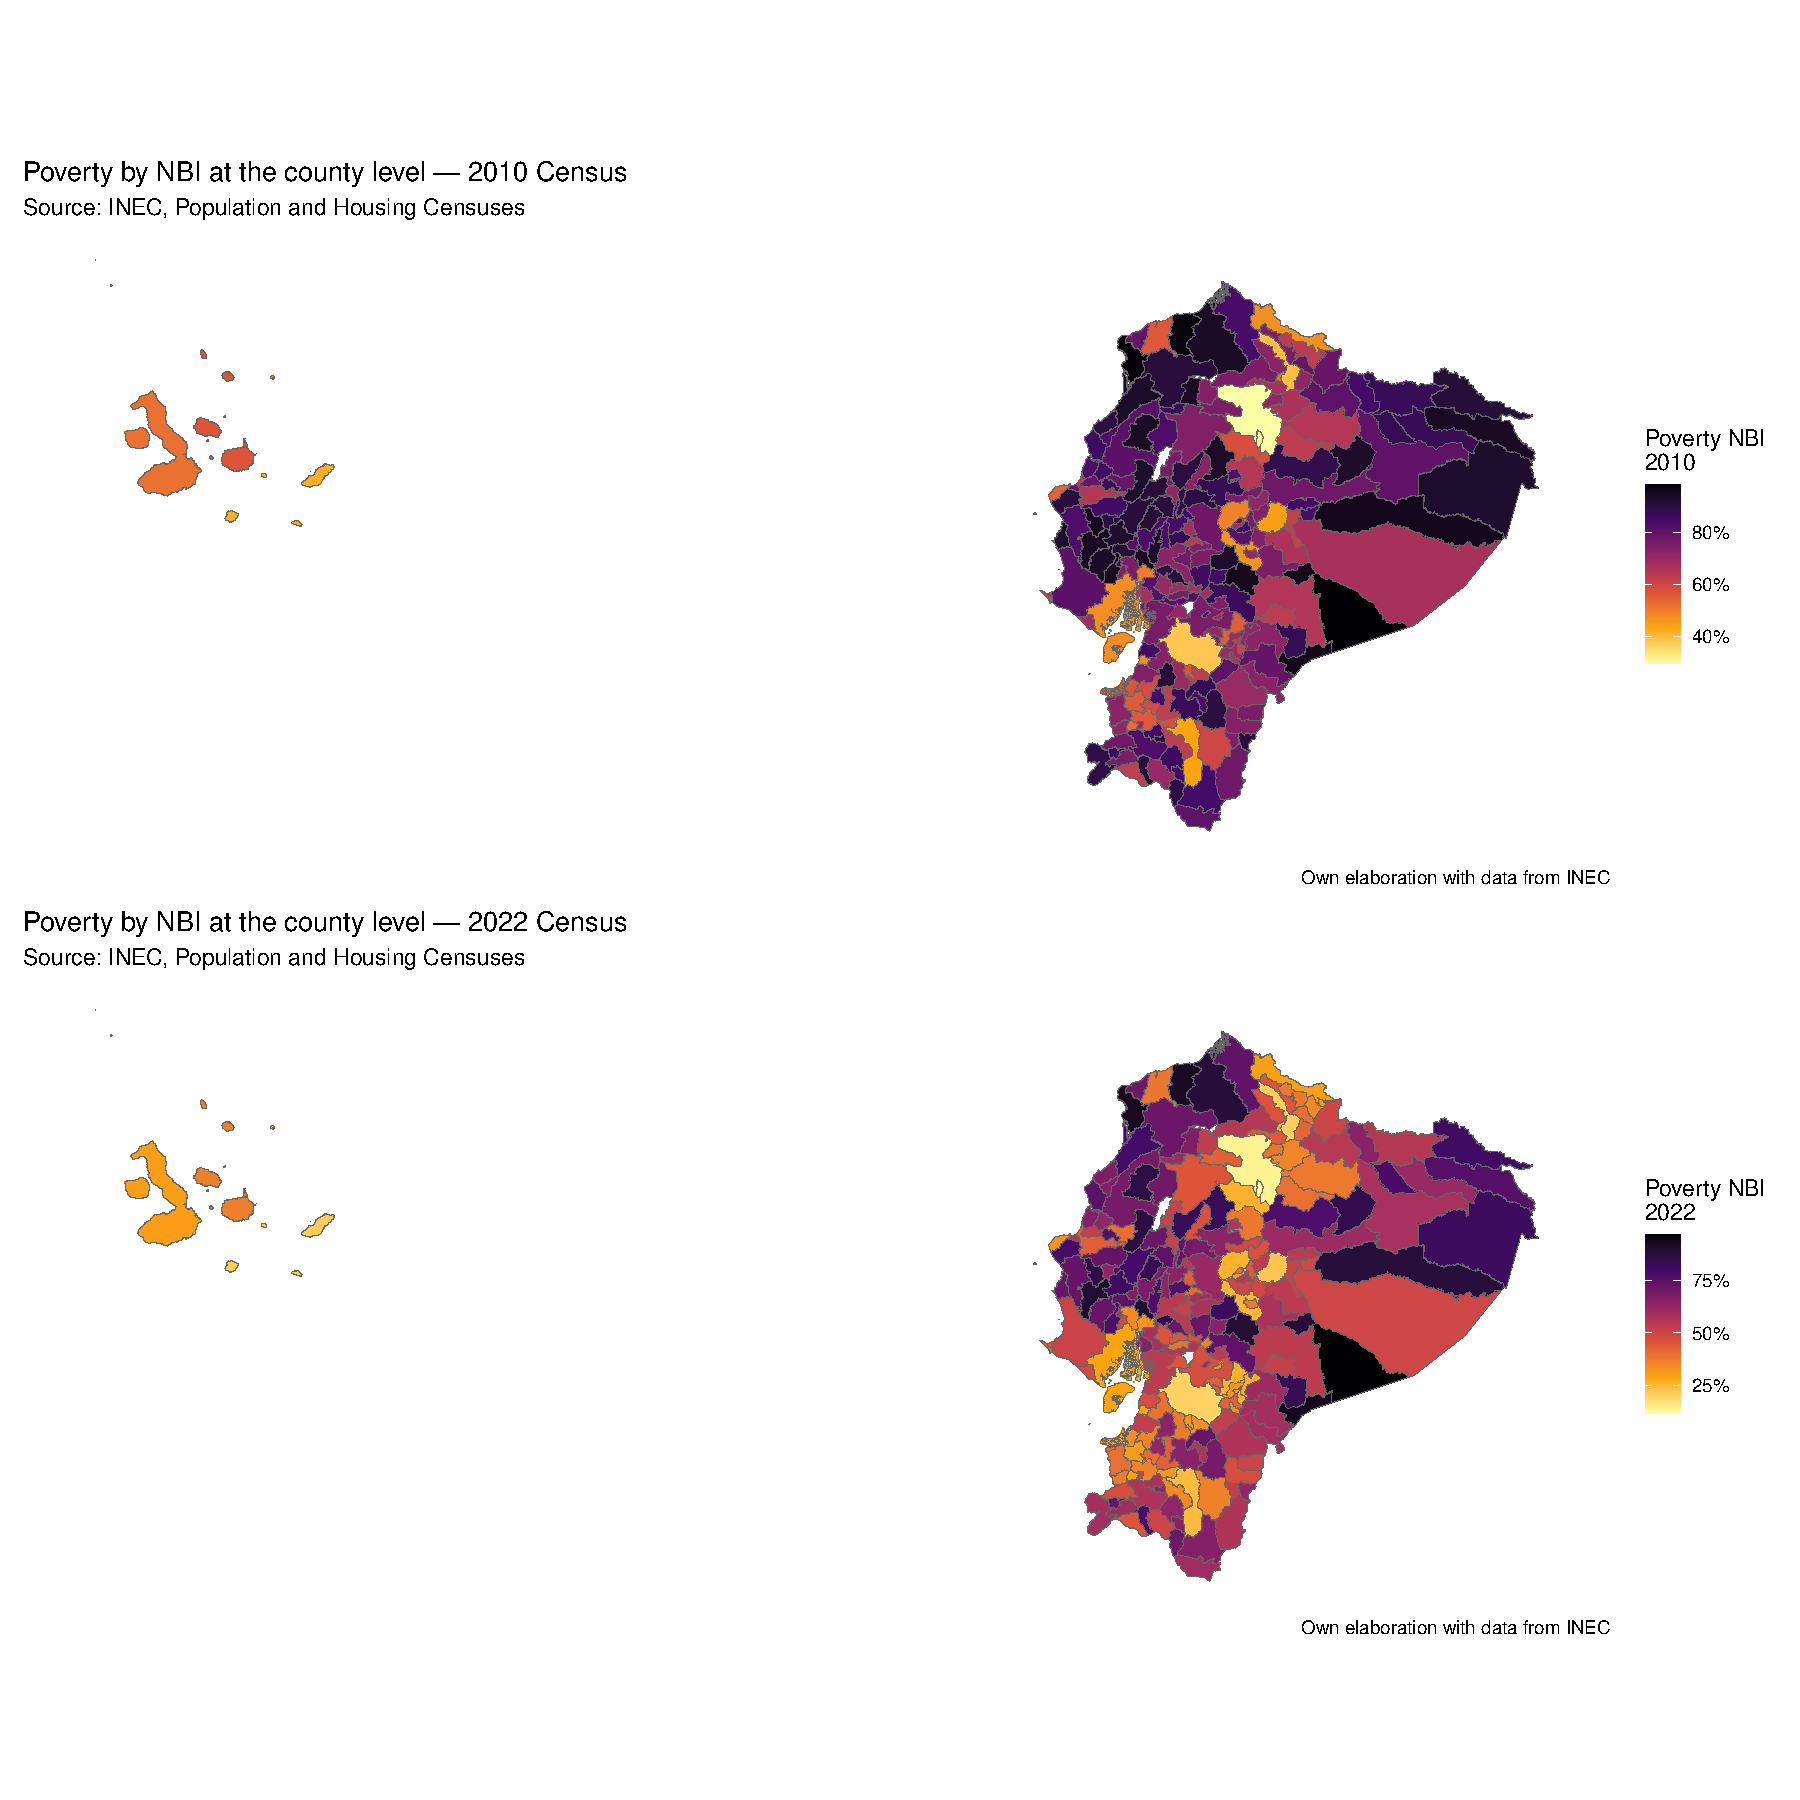
\includegraphics[width=0.70\linewidth]{Fig1.pdf}
    \caption{UBN poverty between 2010 and 2022}
    \label{fig:UBN}
\end{figure}

These group-level aggregates conceal even sharper spatial dispersion, which constitutes the core empirical motivation for canton-level prediction. At the provincial level, the Amazon region has the highest poverty prevalence, with all provinces exceeding 45 percent in 2022. The Sierra registers generally lower rates, though Bol\'{i}var (58.6 percent) and Cotopaxi (48.6 percent) stand out, and the Costa displays pronounced heterogeneity, with Esmeraldas, Manab\'{i}, and Los R\'{i}os exhibiting rates between 60 and 70 percent, while Guayas and El Oro remain below 45 percent \citep{INEC2024NBI}. At the canton level, dispersion is extreme: only 8 of Ecuador's 221 cantons had poverty below 25 percent in 2022, whereas 24 exceeded 80 percent. Figure~\ref{fig:UBN} illustrates the geographic distribution of UBN poverty in 2010 and 2022. Comparing the two census rounds, the Sierra recorded substantial poverty reductions, whereas the Amazon experienced comparatively slow progress. Canton-level dynamics are also heterogeneous, with some cantons remaining in extreme deprivation or experiencing minimal progress while others achieved large reductions. This dispersion implies that models with strong aggregate performance may still be inadequate for policy if they systematically mismeasure poverty in persistently deprived or rapidly changing peri-urban cantons, highlighting the need to evaluate predictive performance across the poverty distribution, particularly in the tails.




\section{Data}
\label{sec:data}

The dataset is defined at the canton level ($N=218$), with the 2022 Census, the most recent available, providing the benchmark poverty rates used for model training and validation.\footnote{The three insular (Gal\'{a}pagos) cantons are excluded, so the analysis covers 218 mainland cantons.} The dataset integrates covariates from three sources: (i) administrative and socioeconomic indicators compiled by INEC; (ii) anonymized, aggregated mobile phone mobility metrics; and (iii) climate-related indicators. The inclusion of mobility metrics alongside administrative covariates is motivated by evidence that mobility patterns encode dimensions of economic activity and spatial connectivity not directly observed in administrative registries, and that they provide higher-frequency signals of local economic dynamics \citep{blumenstock2015predicting, hernandez2017estimating, scepanovic2015mobile}. The resulting feature space is deliberately high-dimensional, reflecting both the richness of available administrative diagnostics and the objective of assessing alternative covariate constructions and regularization strategies. Throughout, ``administrative benchmark'' refers to the full set of 947 official and environmental indicators; it does not imply that every covariate originates in an administrative register.

Table~\ref{tab:data} summarizes the data scenarios used in the model grid. The baseline specification includes 947 indicators covering education, health, real sector activity, financial inclusion, socioeconomic conditions, security, labor, and environmental dimensions related to climate and deforestation. Scenarios (2) and (3) add mobile phone mobility indicators to the baseline, entered either as canton averages or as their first principal component. Scenario (4) relies exclusively on mobility data. Together, these scenarios separate the standalone predictive content of mobility from its incremental contribution relative to a rich set of administrative covariates. The large and uneven number of indicators across domains reflects the structure of the official compilation and should not be read as the substantive weight of each domain in deprivation. Appendix~\ref{app:Mobility} provides further details on the mobility indicators, and Online Resource 1 documents the complete set of predictors, reporting the area, data source, and a descriptive name for each variable.\footnote{The 2022 Population and Housing Census is used to construct the UBN outcome, but no variables taken directly from the Census are included as predictors. This rules out direct reuse of 2022 Census covariates in the prediction models, although the comparison remains subject to the reference dates and constructions of the different sources. The mobility indicators are derived from telecommunications records and statistically expanded using official INEC cantonal population projections.}

\begin{table}[!htbp]
\centering
\begin{tabular}{p{3.5cm} p{2.5cm} p{7cm} p{1.5cm}}
\toprule
\textbf{Name} & \textbf{Scenario} & \textbf{Description} & \textbf{N} \\
\midrule

\textbf{Baseline}
& (1)
& 947 administrative, socioeconomic, and environmental indicators compiled by INEC from multiple official sources and organized into eight domains: education (426), health (265), real sector activity (86), financial inclusion (61), socioeconomic conditions (52), security (46), climate change and deforestation (9), and labor (2).
& 947 \\

\midrule

\textbf{Baseline with \newline mobility data}
& (2)
& Baseline data augmented with mobility indicators:
internal traffic (19) and national traffic (19).
& 947 + 38 \\

\midrule

\textbf{Baseline with \newline mobility factor}
& (3)
& Baseline data augmented with the first principal component of the mobility indicators (based on averages).
& 947 + 1 \\

\midrule

\textbf{Mobility data}
& (4)
& Mobility indicators (averages): internal traffic (19) and national traffic (19).
& 38 \\

\bottomrule
\end{tabular}
\caption{Data Scenarios and Variable Composition}
\label{tab:data}
\end{table}

\subsection{Mobile Phone Mobility Data}

The mobile phone mobility data are derived from anonymized network connection records containing timestamps and cell-site locations for active subscribers, processed through a multi-stage pipeline comprising anonymization, spatial aggregation, and statistical expansion, in compliance with Ecuador's data protection law.\footnote{Ley Org\'{a}nica de Protecci\'{o}n de Datos Personales.} The platform discretizes national territory into a regular hexagonal grid (hx8), where each hexagon has an internal circumradius of approximately 500 meters. This tessellation yields homogeneous spatial units that are comparable across urban and rural contexts and can be consistently intersected with other spatial layers, although it does not eliminate sensitivity to aggregation boundaries. All spatial outputs are provided in the WGS 1984 geographic coordinate reference system (EPSG:4326), ensuring interoperability with official census cartography and national geospatial datasets.

Origin--destination (OD) flows are inferred from individual \textit{estad\'{i}as}, defined as the ordered sequence of network locations at which a subscriber is registered within a given day. For subscribers observed at multiple locations in a day, successive location changes are treated as trips, each assigned temporal attributes (hour of day and day of week). To scale flows to population totals, an expansion factor is computed at the origin hexagon by allocating official INEC cantonal population projections across constituent hx8 units in proportion to the relative density of observed clients; this factor is then applied to each outbound trip record. The expansion scales recorded flows to population totals but does not by itself ensure that observed subscribers represent all residents in their mobility behavior. The expanded trip table is aggregated along multiple temporal dimensions, including total flows; day of week; weekday versus weekend; and intra-day bands (morning, afternoon, evening, night), separately for weekdays and weekends. For each temporal dimension, two complementary measures are constructed: \textit{viajes} (trip counts) and \textit{viajeros} (unique travelers), summarizing mobility intensity and participation.

Figure~\ref{fig:movilidad_map} shows the mobility routes. In a subsequent processing stage (\textit{Rutas \'{O}ptimas}), OD flows between hx8 zone pairs are projected onto the national road network to recover least-cost paths, thereby disaggregating zonal flows into segment-level traffic intensities. In the source product, each road segment is further enriched with sociodemographic attributes (age cohort, socioeconomic stratum, and user type) derived from Client 360 profiling of the underlying subscriber base. These attributes are not used in the estimated models, which rely on the 38 aggregated mobility measures documented in Table~\ref{tab:data}.

\begin{figure}[!htbp]
    \centering
    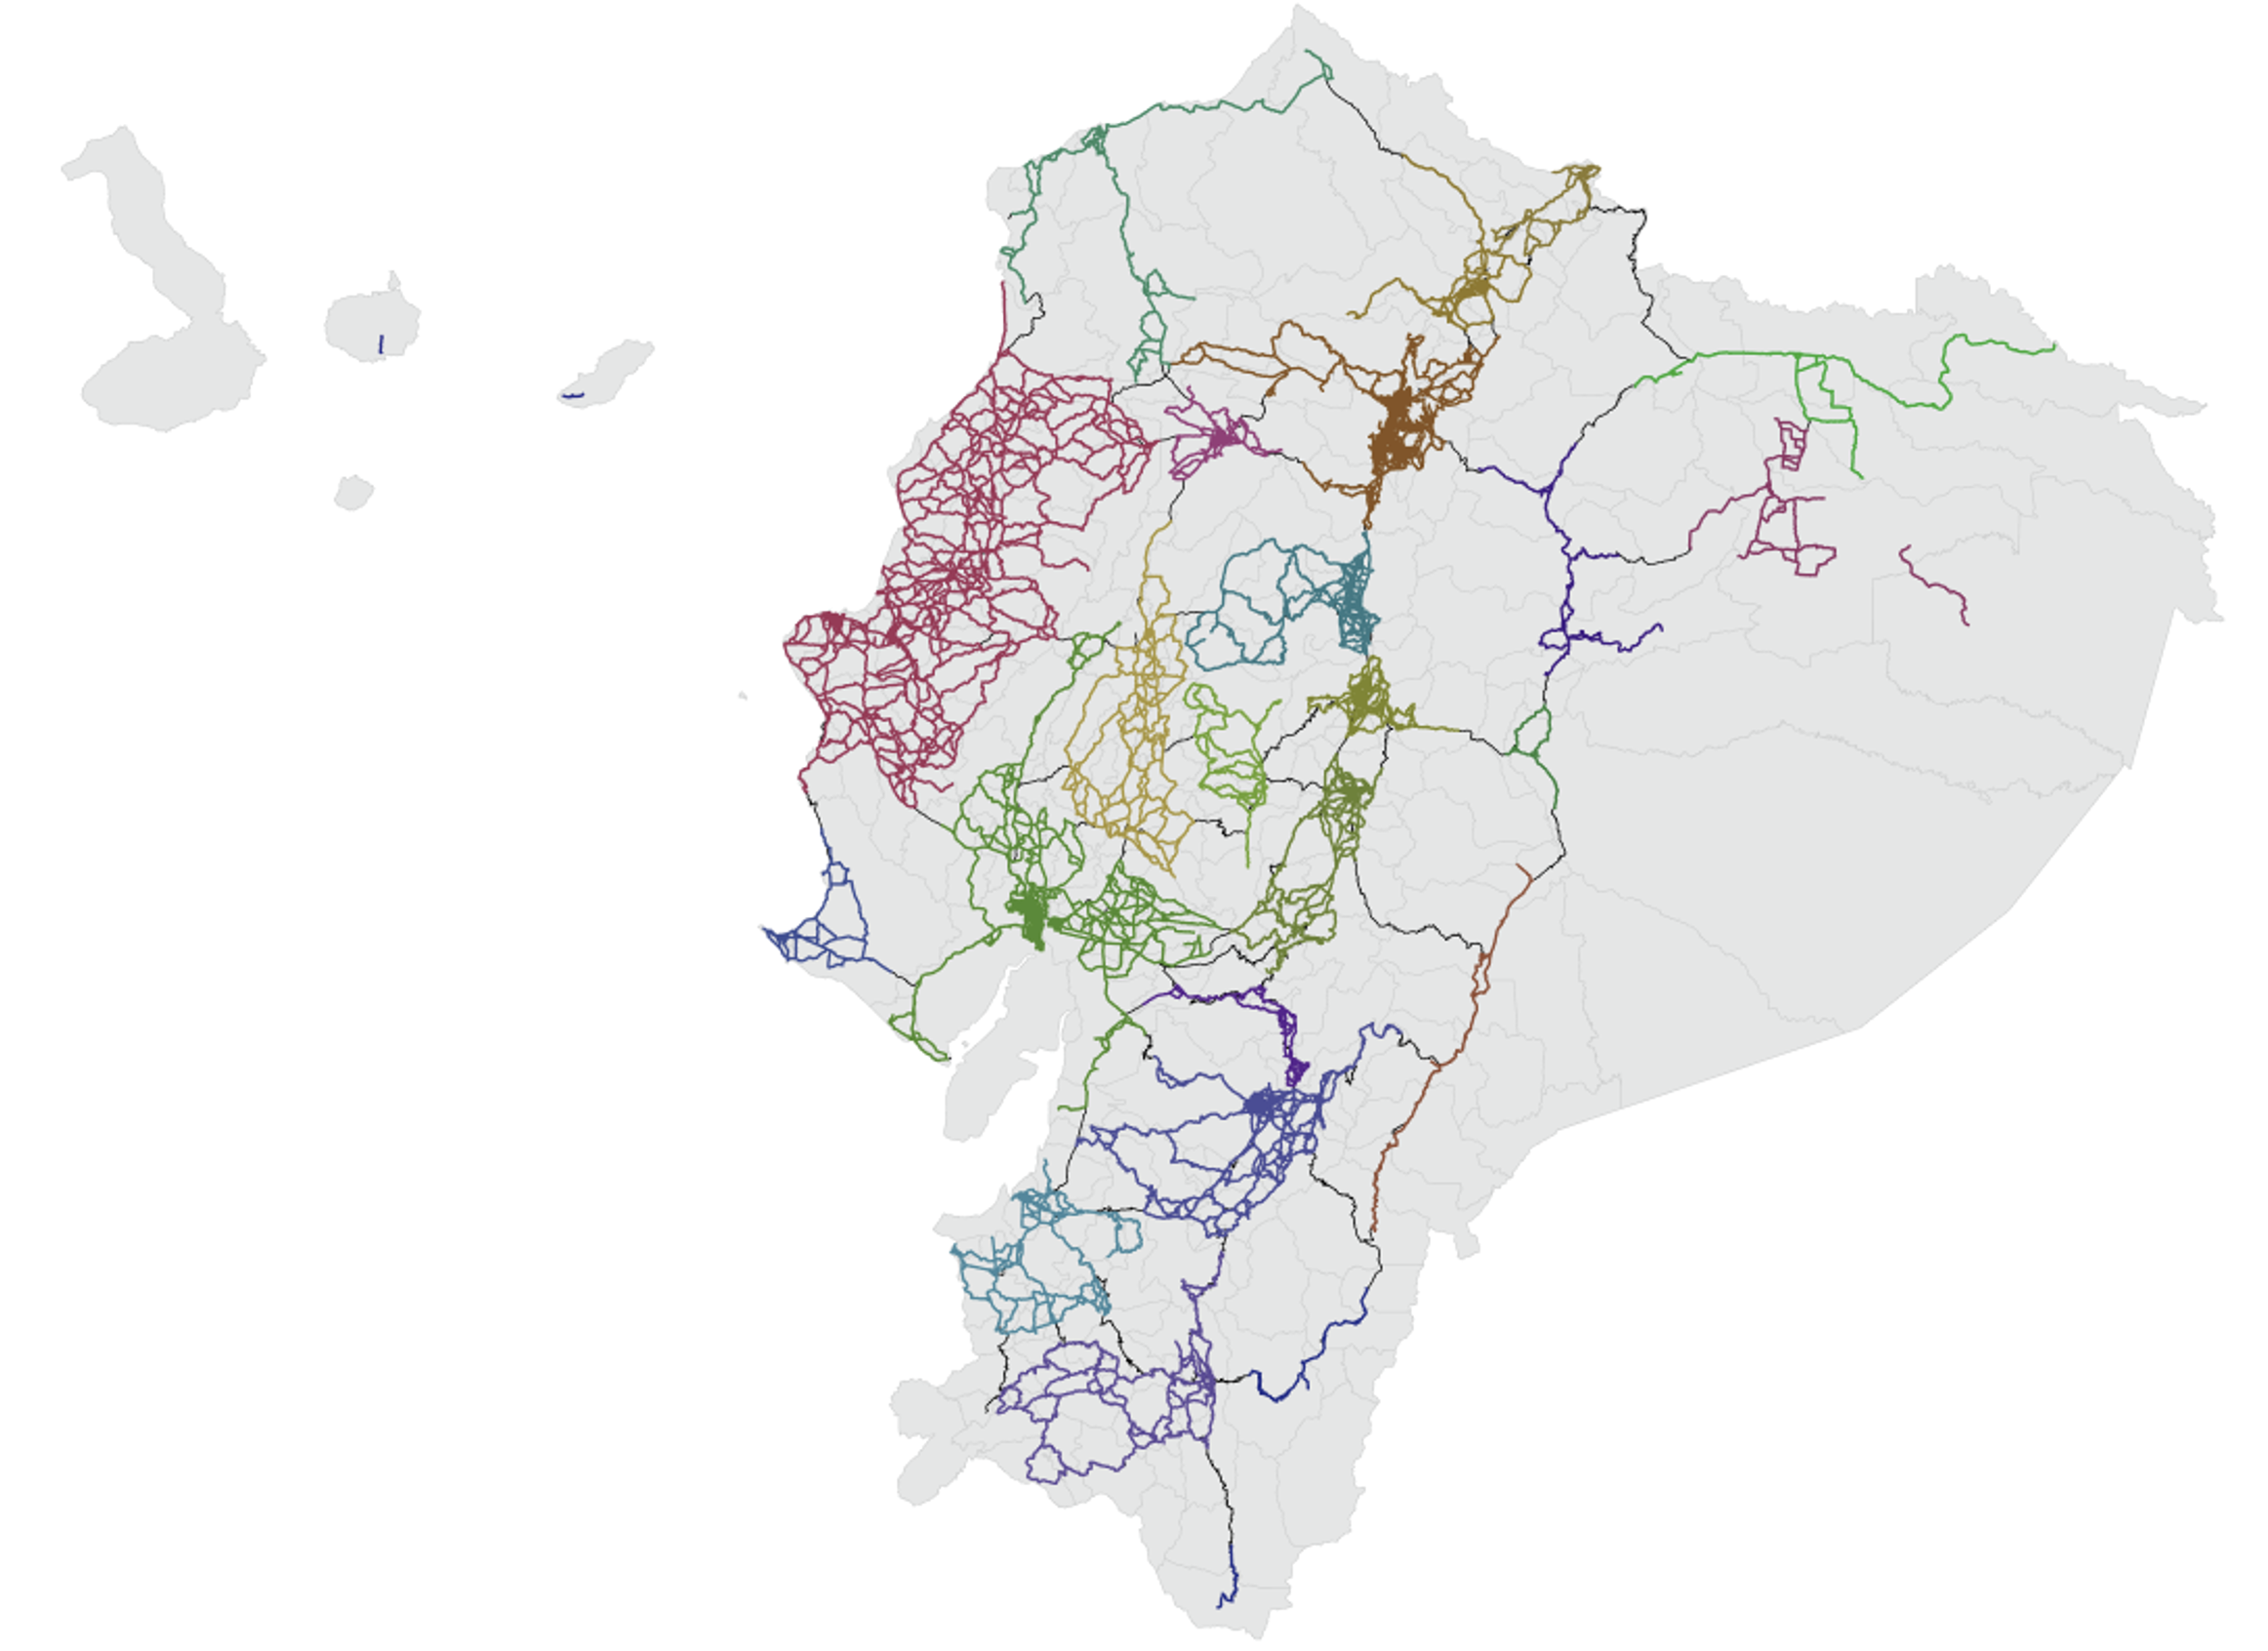
\includegraphics[width=0.5\textwidth]{Fig2.png}
    \caption{Optimal mobility routes derived from the phone geodatabase for Ecuador, June 2024. Each line represents a road segment identified as part of an optimal route connecting origin--destination pairs. Colors distinguish the 24 provincial layers contained in the geodatabase. The spatial concentration of route density in the Sierra corridor (notably Pichincha, Tungurahua, and Azuay) and along the coastal lowlands (Guayas and Manab\'{i}) reflects the underlying population distribution and the intensity of recorded subscriber movements. Sparsely covered areas in the eastern Amazonian provinces (Orellana, Sucumb\'{i}os, Pastaza, Morona Santiago, and Zamora Chinchipe) are consistent with lower population density and reduced mobile network penetration in those territories. The Gal\'{a}pagos Islands (upper-left inset) exhibit minimal route coverage due to their small, geographically isolated population. All geometries are projected in WGS 1984 (EPSG:4326). \textit{Note: Map not to scale}}
    \label{fig:movilidad_map}
\end{figure}

The resulting mobility layers are stored in a geodatabase comprising 25 MultiLineString vector layers (24 provincial layers and one interprovincial layer) corresponding to the June 2024 snapshot. Each layer follows a tidy data schema that links individual road segments to a single thematic filter, variable level, and numeric value. For this paper, segment-level mobility indicators are aggregated to the canton level (218 mainland cantons) using their mean values. This produces 38 covariates: 19 internal-flow and 19 national-flow measures. In Scenarios (2) and (4), all 38 measures enter the model. In Scenario (3), the first mobility principal component is estimated anew within each training fold and then applied to the corresponding held-out fold, preventing information leakage.

\subsection{Reference Dates and Structural Deprivation}
\label{subsec:reference_dates}

The census outcome refers to 2022, whereas the mobility snapshot refers to June 2024. The interpretation of this comparison rests on the structural character of UBN. Housing characteristics, water and sanitation infrastructure, and crowding largely reflect accumulated resources and past investment, while aggregate mobility reflects the spatial arrangement of settlements, transport connections, and economic opportunities. These shared territorial characteristics can make a later mobility snapshot informative about an earlier deprivation distribution even if specific behaviors change. This rationale is consistent with evidence that phone data predict structural measures of wealth and multidimensional poverty more accurately than transient welfare outcomes \citep{Smith2026Wellbeing}, but it does not establish that the particular indicators used here are stable over time.

The estimand is therefore the accuracy with which each information set recovers observed 2022 census deprivation in geographically excluded cantons. Because the objective is predictive association rather than a causal effect or a forecast available in 2022, a predictor measured after the census can be evaluated for this retrospective spatial task. The timing difference nonetheless remains relevant for interpretation: \citet{aiken2022machine} document deterioration in phone-based targeting performance when data or models become outdated. If anything, the two-year gap could attenuate the incremental contribution of mobility, a point we return to in Section~\ref{sec:conclusion}.


\section{Empirical Strategy}
\label{sec:methods}

This section presents the empirical strategy for predicting canton-level poverty when candidate predictors greatly outnumber geographic units. The framework has three elements: transformations that control dimensionality and multicollinearity; linear and nonlinear prediction models; and nested spatial cross-validation to evaluate prediction accuracy and signed error in geographically held-out regions.

\subsection{Machine Learning Framework}

Let $\mathbf{X}_i=[X_{1i},X_{2i},\dots,X_{ki}]$ denote the high-dimensional covariate vector for canton $i=1,2,\dots,218$, and let $y_i$ denote the corresponding UBN poverty rate. Following \citet{GouletCoulombe2021, GouletCoulombe2022}, the prediction problem can be expressed as
\begin{equation}
y_i = g(f(\mathbf{X}_i)) + \varepsilon_i,
\label{eq:poverty_problem}
\end{equation}
where $f(\cdot)$ denotes a transformation of the covariate space used to address high dimensionality, $g(\cdot)$ is the prediction function mapping transformed covariates into poverty, and $\varepsilon_i$ represents residual variation under the specified representation. These are prediction tools and do not identify structural causal relationships.

A natural benchmark is $f(\mathbf{X}_i)=\mathbf{X}_i$, implying no transformation. However, when $k$ is large relative to $n$, and particularly when predictors are highly correlated, unregularized linear estimation is infeasible or unstable and prone to overfitting. This motivates two classes of strategies for $f(\cdot)$. The first uses regularization methods that select or shrink predictors, such as LASSO \citep{Tibshirani1996}. The second uses factor extraction to reduce dimensionality, such as principal component regression (PCR) and partial least squares (PLS). Standard principal components are unsupervised: they maximize variance in $\mathbf{X}$ rather than predictive relevance for $y$. When only a subset of covariates is informative for the outcome, unsupervised factor extraction can be inefficient or even inconsistent \citep{Bair2006}. We therefore also consider supervised factor extraction through PLS \citep{WOLD1973, Hastie2009} and ``targeted predictors'' designs that apply PCR to covariates preselected by LASSO \citep{bai2008forecasting}.

The second component of the framework is the choice of $g(\cdot)$. A linear functional form imposes a parametric relationship between the transformed covariates and poverty and can be attractive when interpretability and stability are priorities. Nonlinear algorithms may deliver greater accuracy by capturing interactions and nonlinearities, and some perform implicit variable selection. We compare linear methods with gradient boosting (XGBoost) under squared-error loss and with an XGBoost variant targeting the conditional median, which provides an alternative loss function that is less sensitive to extreme observations \citep{chen2016xgboost}.

Let the underlying conditional representation be $y_i = g^*(f^*(\mathbf{X}_i))+ \varepsilon_i$ and let the estimated predictor be $\hat{y}_i=\hat{g}(\hat{f}(\mathbf{X}_i))$. The prediction error decomposes as
\begin{align}
y_i - \hat{y}_i
&= \underbrace{g^*(f^*(\mathbf{X}_i)) - g(f(\mathbf{X}_i))}_{\text{Approximation error}}
+ \underbrace{g(f(\mathbf{X}_i)) - \hat{g}(\hat{f}(\mathbf{X}_i))}_{\text{Estimation error}}
+ \varepsilon_i.
\label{eq:error_decomposition}
\end{align}
The first component is approximation error, which arises from the choice of transformation $f(\cdot)$ and functional form $g(\cdot)$ and persists even with large samples. The second is estimation error, which reflects the recovery of these objects from a finite training sample. Census coverage removes sampling error from the measured outcome, but it does not make estimation error negligible: each spatial training sample contains fewer than 218 cantons, and variable selection, factor extraction, and tuning can vary across those samples. Nor does census coverage rule out nonsampling error in the outcome itself. The evaluation therefore treats the observed census rate as the benchmark and measures OOS prediction error relative to it. Our primary question is whether mobility adds information beyond a high-dimensional administrative benchmark; our secondary question is whether model and covariate choices preserve differences across the observed poverty distribution.

We implement five covariate designs: the full predictor set, PCR, PLS, LASSO selection, and principal components extracted after LASSO selection. We combine these designs with three models (a linear model, XGBoost with squared-error loss, and XGBoost targeting the conditional median) under four data scenarios. The designs address high dimensionality and multicollinearity, while the model comparison separates the effect of transforming the predictor space from the effect of allowing nonlinearities and interactions.

PCR constructs a low-dimensional representation of the covariate space by extracting orthogonal components that summarize common variation in the predictors, and then estimates a linear mapping from these components to poverty \citep{Hastie2009}. Although this approach substantially reduces dimensionality, components are chosen to maximize variance in the covariates rather than predictive relevance. PLS addresses this limitation by extracting components that maximize covariance with the outcome, incorporating predictive relevance directly into the construction of the factor space \citep{WOLD1973, Hastie2009}. This is useful when outcome-relevant information is concentrated in specific combinations of covariates rather than in the dominant modes of variation in the predictor matrix.

LASSO imposes an $\ell_1$ penalty that shrinks many coefficients to zero, yielding parsimonious specifications that serve either as final predictive models or as feature-selection stages \citep{Tibshirani1996}. Building on this approach, the targeted factor design extracts principal components only from the subset of covariates selected by LASSO. This restricts factor extraction to predictors with demonstrated relevance to the outcome and mitigates the risk that unsupervised PCR focuses on variation unrelated to poverty \citep{bai2008forecasting, Bair2006}.

XGBoost constructs an additive ensemble of decision trees estimated by gradient boosting with explicit regularization, allowing flexible functional forms and interactions that are difficult to capture with linear models \citep{chen2016xgboost}. The median variant replaces squared-error loss with quantile loss at the median. It is included as an alternative prediction objective and is not presumed to correct errors across the poverty distribution.

Hyperparameter tuning strategies are summarized in Online Resource 2. All tunable parameters are selected by Bayesian optimization on the inner spatial folds of the nested spatial cross-validation described in Section~\ref{subsec:evaluation} \citep{Bergstra2011}. The tuning objective is mean squared error for the linear and squared-error XGBoost models and median quantile loss for the median XGBoost model. For each covariate design, all preprocessing, dimension-reduction, variable-selection, and tuning steps are performed exclusively on the training sample. The resulting transformations and fitted models are then applied to the held-out sample, ensuring that it remains uncontaminated by information used during estimation.

\subsection{Covariate Designs and Data Scenarios}

Table~\ref{tab:designs_summary} summarizes the five covariate designs. The designs differ in the transformation $f(\mathbf{X})$ applied before estimation. The ``full'' design uses all available covariates; PCR and PLS extract low-dimensional factor spaces; LASSO selects a subset of covariates; and the hybrid \texttt{pcr\_lasso} design applies PCR to the covariates selected by LASSO.

\begin{table}[!htbp]
    \centering
    \small
    \begin{tabular}{lp{10cm}l}
        \toprule
        \textbf{Name} & \textbf{Description} & \textbf{Method} \\
        \midrule
        full & All original variables in $\mathbf{X}$. & None \\
        pcr & Principal components estimated from $\mathbf{X}$ via nested spatial CV. & PCR \\
        pls & Factors extracted via PLS using all variables in $\mathbf{X}$ via nested spatial CV. & PLS \\
        lasso & Variable selection from $\mathbf{X}$ with LASSO via nested spatial CV. & LASSO \\
        pcr\_lasso & Variable selection with LASSO from $\mathbf{X}$ followed by PCR on selected variables. & PCR and LASSO \\
        \bottomrule
    \end{tabular}
    \caption{Covariate Designs}
    \label{tab:designs_summary}
\end{table}

Combining the five covariate designs with the four data scenarios in Table~\ref{tab:data} and the three prediction algorithms yields the evaluation grid. Because the full design cannot be fitted by unregularized linear regression, the number of estimated specifications per scenario is $5 \times 3 - 1 = 14$, giving a total of $14 \times 4 = 56$ model specifications.

\subsection{Spatial Evaluation}
\label{subsec:evaluation}

To account for spatial dependence, we use nested spatial cross-validation \citep{Mahoney2023}. This design is especially relevant in our application because nearby cantons often share similar economic, demographic, and geographic conditions. Under ordinary random cross-validation, neighboring cantons may appear in both the training and test samples, making prediction artificially easy and yielding overly optimistic estimates of OOS performance. The 218 cantons are partitioned into five spatially contiguous outer folds using $k$-means clustering of canton locations (Figure~\ref{fig:spatial_folds}). For each outer fold, five inner spatial folds constructed from the remaining territories are used to select all supervised transformations and hyperparameters without using the eventual test region. The model is then refitted on the outer training sample with the selected configuration and used to predict the held-out fold. If $s(i)$ denotes the outer spatial fold containing canton $i$, its prediction is
\begin{equation}
\hat{y}^{\mathrm{OOS}}_i=\hat{g}_{-s(i)}\big(\hat{f}_{-s(i)}(\mathbf{X}_i)\big),
\label{eq:oos_prediction}
\end{equation}
where the subscript $-s(i)$ indicates estimation without the fold containing canton $i$. Concatenating the five outer test sets produces one geographically OOS prediction for every canton and therefore a complete OOS poverty map.

This design separates model selection from geographic evaluation. The inner folds prevent the outer test region from affecting scaling, PCR or PLS construction, LASSO selection, and hyperparameter tuning. The contiguous outer folds test transfer to unseen regions rather than interpolation among neighboring training units. The exclusion is geographic, not temporal.

Our primary accuracy metric is the spatial OOS RMSE, expressed in percentage points of UBN poverty:
\begin{equation}
\text{RMSE}^{\text{OOS}}_{m}
=
100\times\sqrt{\frac{1}{n} \sum_{i=1}^{n} \left( \hat{y}^{\text{OOS}}_{i}-y_{i} \right)^2},
\label{eq:rmse}
\end{equation}
where $m$ denotes the model, $y_{i}$ is the 2022 census UBN poverty rate of canton $i$ (as a proportion), $\hat{y}^{\text{OOS}}_{i}$ is its OOS prediction, and $n=218$. This pooled measure gives each canton equal weight. As an overfitting diagnostic, Online Resource 2 reports the gap between in-sample and spatial OOS RMSE; in-sample fit is never treated as predictive evidence.

To assess distributional performance, we compute the OOS signed error for a set of cantons $G$:
\begin{equation}
\text{Bias}_{m,G} = \frac{100}{|G|} \sum_{i \in G} \left( \hat{y}^{\text{OOS}}_{i} - y_{i} \right),
\label{eq:signed_error}
\end{equation}
where a positive value indicates overprediction and a negative value indicates underprediction. Compression of the poverty distribution therefore appears as positive signed error in low-poverty groups and negative signed error in high-poverty groups.\footnote{We retain the term ``bias'' for correspondence with the figures, but this quantity describes realized systematic error across cantons in the OOS predictions; it is not repeated-sampling bias in the design-based sense used by \citet{Corral2025}.} Population-weighted local regressions are used to describe how signed error varies with observed deprivation; equal weighting in the pooled RMSE and population weighting in the local curves answer different descriptive questions.

To summarize the incremental contribution of mobility, we define the paired accuracy difference
\begin{equation}
\Delta\mathrm{RMSE}_{m}
=\mathrm{RMSE}^{\mathrm{OOS}}_{m,A+M}
-\mathrm{RMSE}^{\mathrm{OOS}}_{m,A},
\label{eq:incremental_rmse}
\end{equation}
where $A$ denotes the administrative benchmark and $M$ denotes either the 38 mobility indicators or their first principal component. Negative values indicate improved accuracy after adding mobility.

\begin{figure}[!htbp]
    \centering
    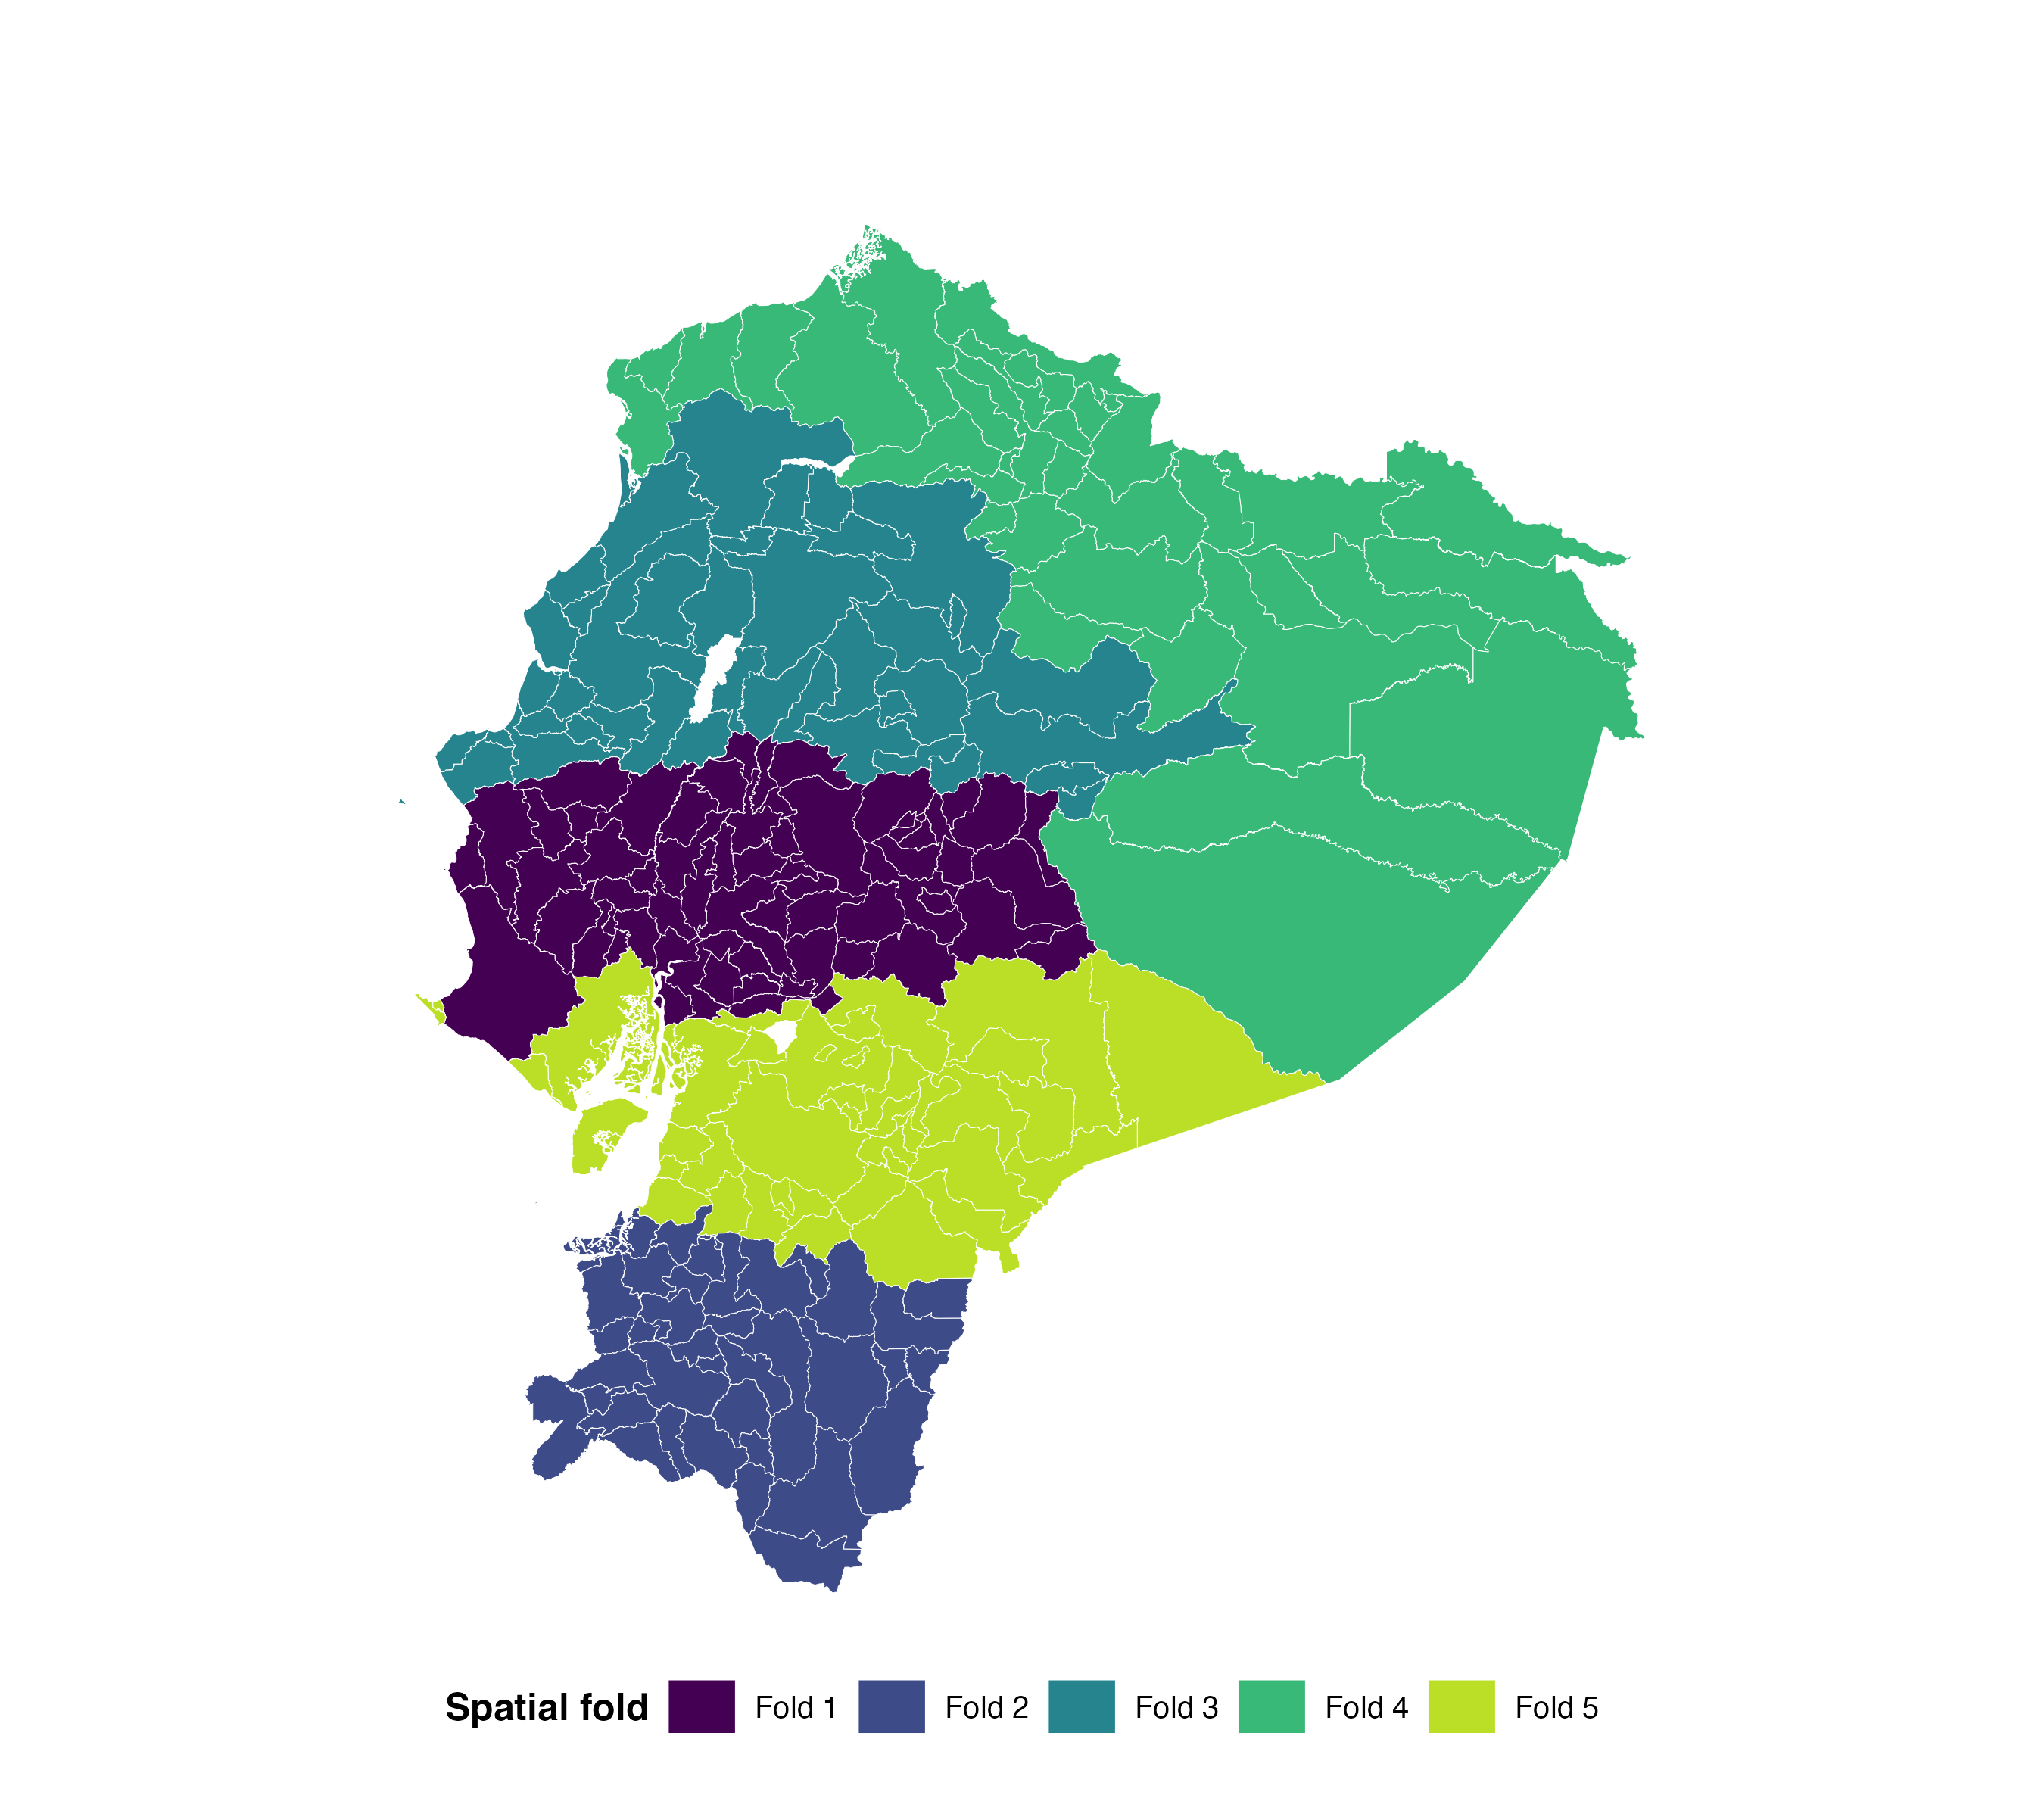
\includegraphics[width=0.6\linewidth]{Fig3.png}
    \caption{Spatial cross-validation folds: the 218 mainland cantons partitioned into five spatially contiguous outer folds used for out-of-sample evaluation}
    \label{fig:spatial_folds}
\end{figure}


\section{Prediction Results}
\label{sec:results}

This section examines whether mobile phone mobility indicators improve poverty prediction in geographically held-out cantons. We first compare average OOS accuracy across data scenarios, covariate designs, and models. We then examine whether prediction errors vary systematically across the poverty distribution, which is particularly important for geographic targeting. Finally, we use feature-attribution measures to describe the main sources of predictive information.

\subsection{Average Predictive Performance}

Figure~\ref{fig:OOS-performance-scenarios} summarizes OOS performance. For each data scenario, it plots the OOS RMSE (left) and signed error (right) of every covariate design and model across the five spatial folds. The fold-level distributions capture sensitivity to the particular regions held out; pooled estimates should therefore be interpreted together with the dispersion and overlap of these distributions, which are descriptive rather than formal tests of equality between models.

First, administrative covariates provide a strong and stable basis for spatial poverty prediction. In the baseline data scenario, the LASSO and full designs under squared-error XGBoost achieve pooled OOS RMSEs of 9.37 and 9.56 percentage points, respectively. Their relatively compact and overlapping fold distributions indicate that both belong to a similarly well-performing group, rather than supporting a precise ranking between them. Regularized linear models attain comparable accuracy but exhibit greater variability across spatial folds. Unsupervised dimension reduction performs noticeably worse: under the administrative baseline, XGBoost RMSE is 14.96 percentage points for PCR, 11.37 for PLS, and 12.38 for PCR after LASSO, consistent with the distinction between maximizing predictor variance and retaining outcome-relevant information \citep{Bair2006, bai2008forecasting}. Predicting geographically held-out cantons is also substantially more demanding than fitting the training data: Online Resource 2 shows that spatial OOS RMSE exceeds in-sample RMSE by 4.7 to 8.6 percentage points across designs, underscoring why in-sample fit is not evidence of predictive accuracy when many indicators are available for few units.

For context, \citet{Corral2025} report a municipality-level RMSE of approximately 8 percentage points for gradient boosting in a Mexican pseudo-census with 1,865 municipalities and 500 repeated survey samples. Their outcome, covariates, geographic scale, and design-based error measure differ from ours, so the two figures cannot be ranked against each other. Their study is relevant here mainly for its emphasis on evaluating predictions against a credible benchmark outcome.

Second, mobility adds no detectable accuracy to the administrative benchmark. Adding mobility indicators, either directly or through their first principal component, produces RMSE distributions that overlap substantially with those obtained using administrative covariates alone. Under the mobility-only scenario, models retain some predictive content across spatial folds, but their RMSE is approximately twice that of the leading administrative specifications and their fold distributions are broader. Mobility is thus a usable standalone proxy, but not a source that improves on the existing information set.

Third, the leading specifications combine low prediction errors with signed errors generally centered near zero. Because positive and negative errors can offset each other, the next section examines whether this aggregate result conceals systematic differences between the least and most deprived cantons.


\begin{figure}[!htbp]
    \centering

    \begin{subfigure}[t]{\textwidth}
        \centering
        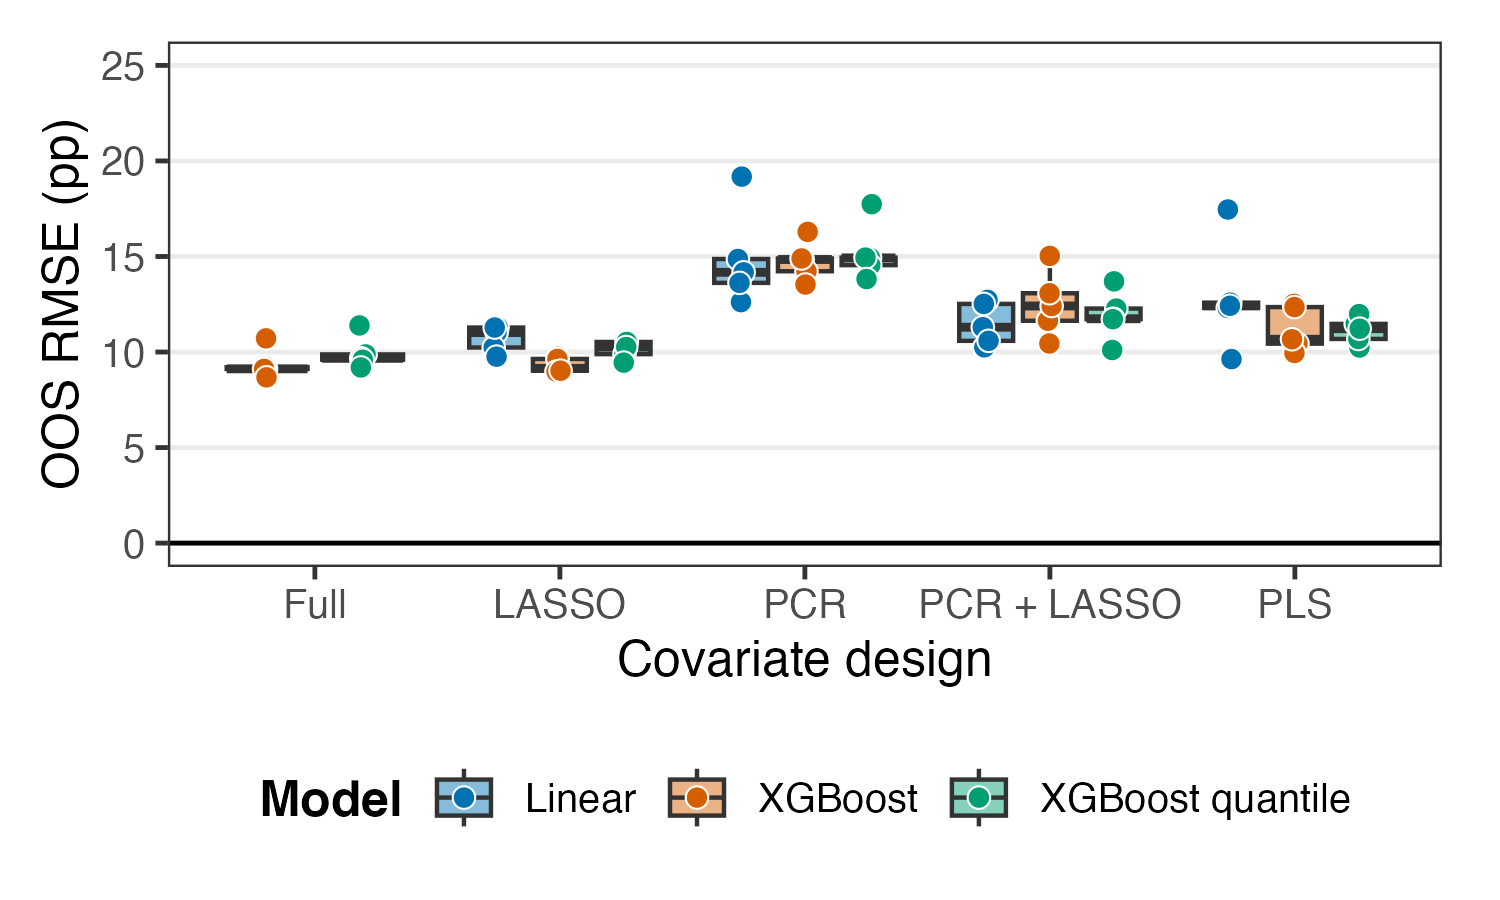
\includegraphics[width=.45\linewidth]{Fig4a_rmse.png}
        \hspace{0.03\linewidth}
        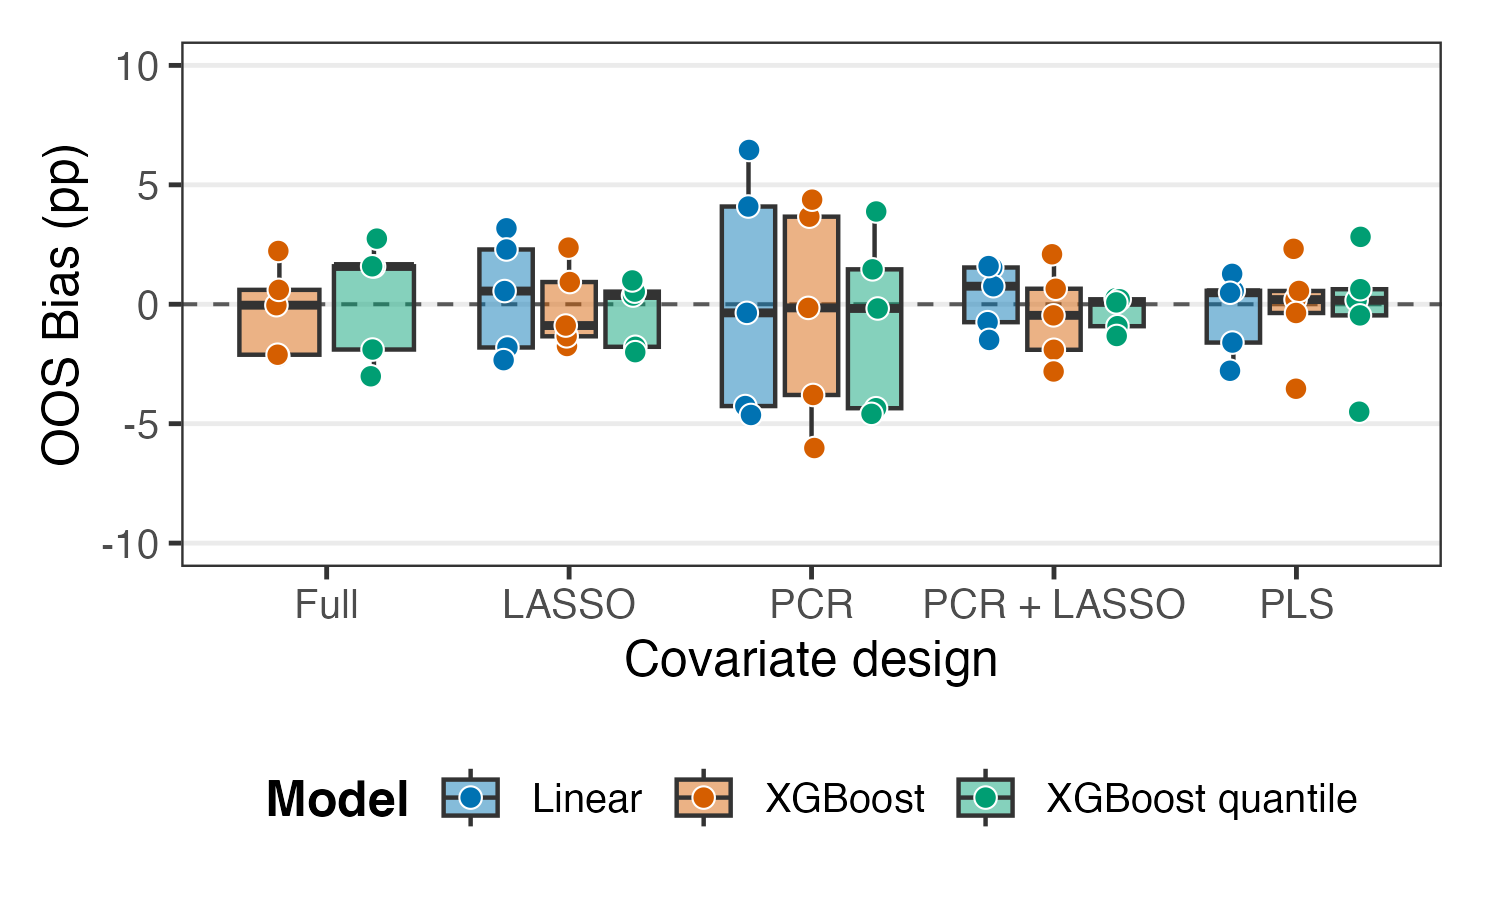
\includegraphics[width=.45\linewidth]{Fig4a_error.png}
        \caption{Data scenario (1): Baseline}
        \label{fig:OOS-baseline}
    \end{subfigure}

    \medskip
    \begin{subfigure}[t]{\textwidth}
        \centering
        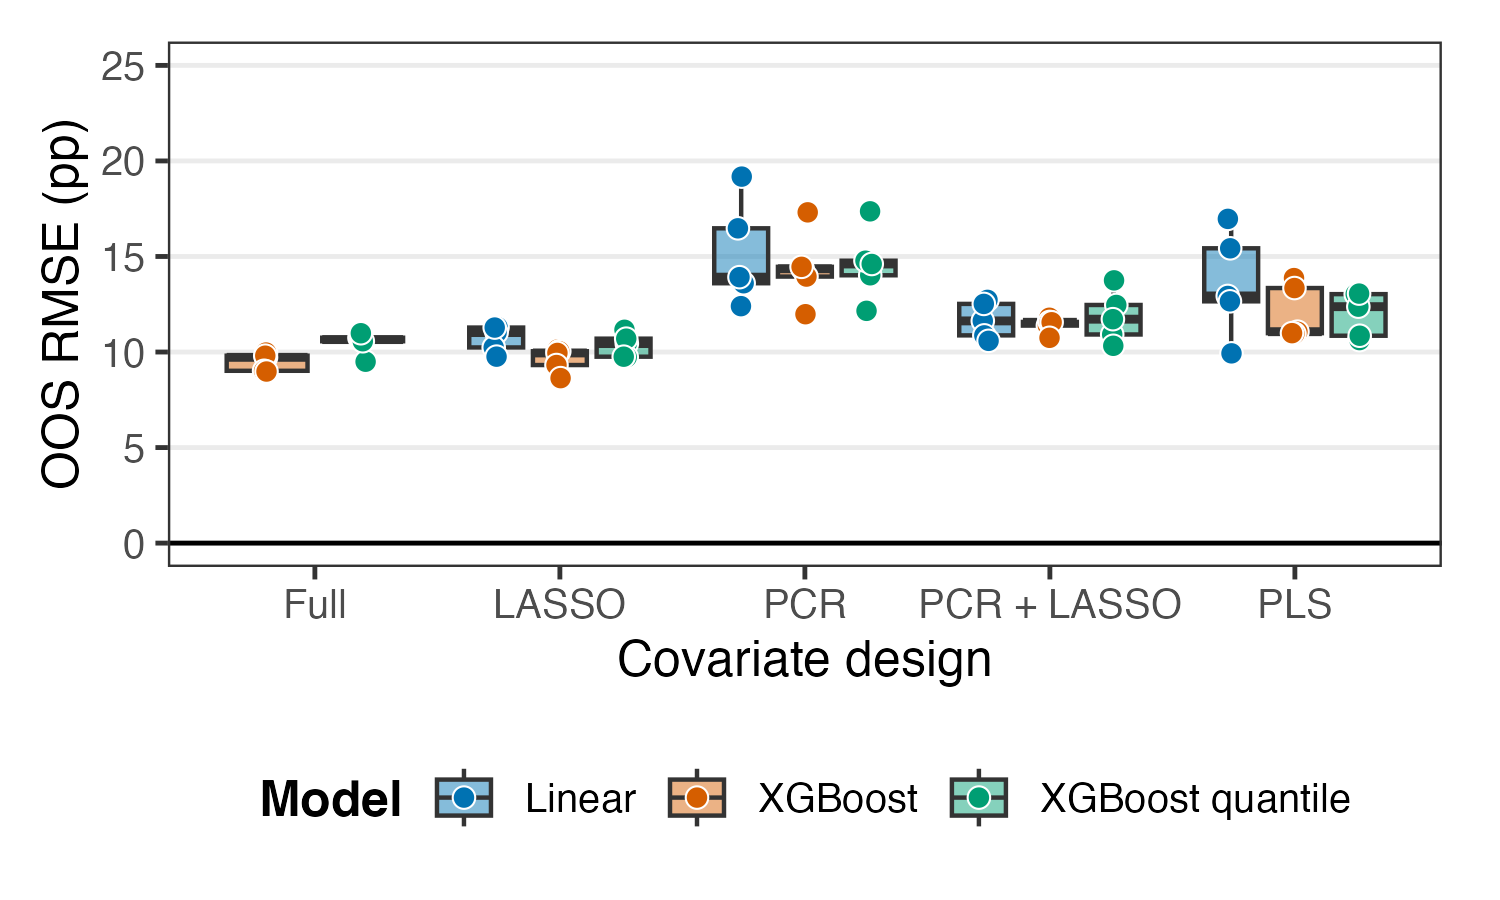
\includegraphics[width=.45\linewidth]{Fig4b_rmse.png}
        \hspace{0.03\linewidth}
        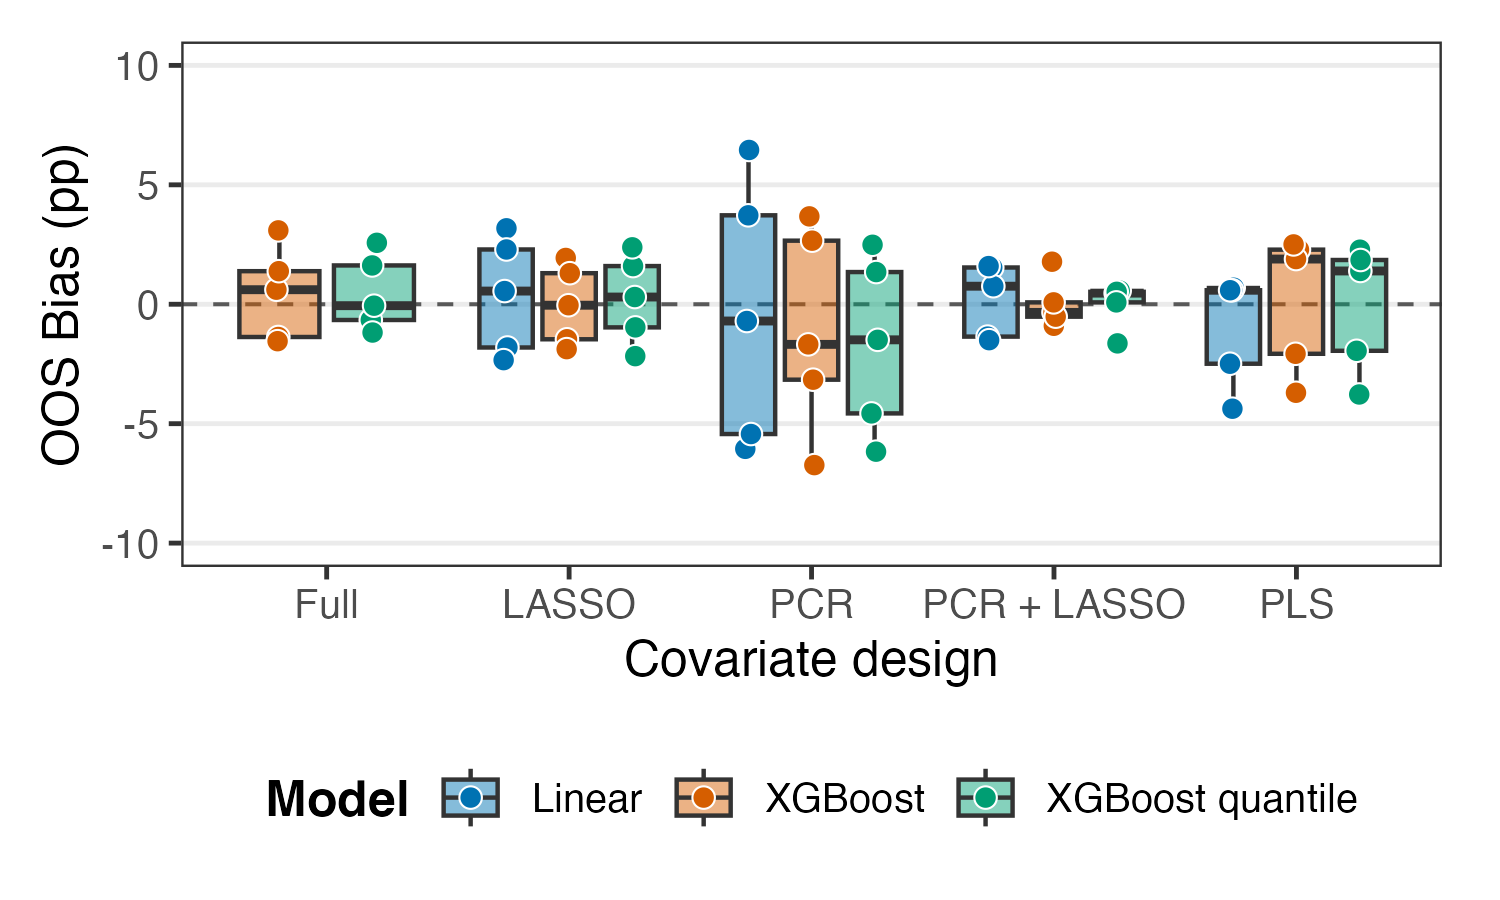
\includegraphics[width=.45\linewidth]{Fig4b_error.png}
        \caption{Data scenario (2): Baseline with mobility data}
        \label{fig:OOS-mobile-mean}
    \end{subfigure}

    \begin{subfigure}[t]{\textwidth}
        \centering
        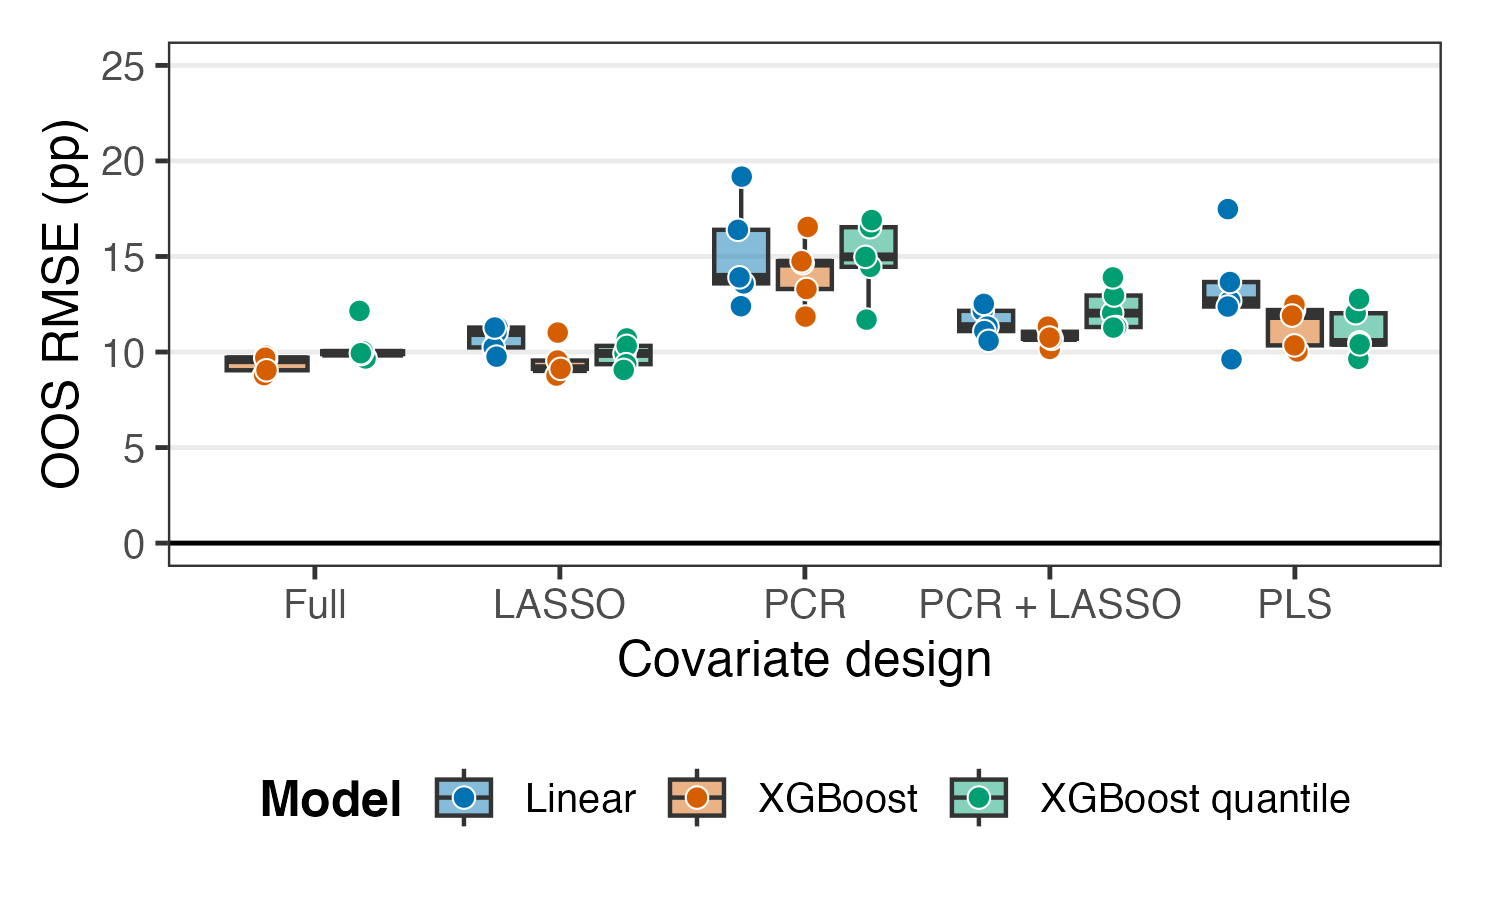
\includegraphics[width=.45\linewidth]{Fig4c_rmse.png}
        \hspace{0.03\linewidth}
        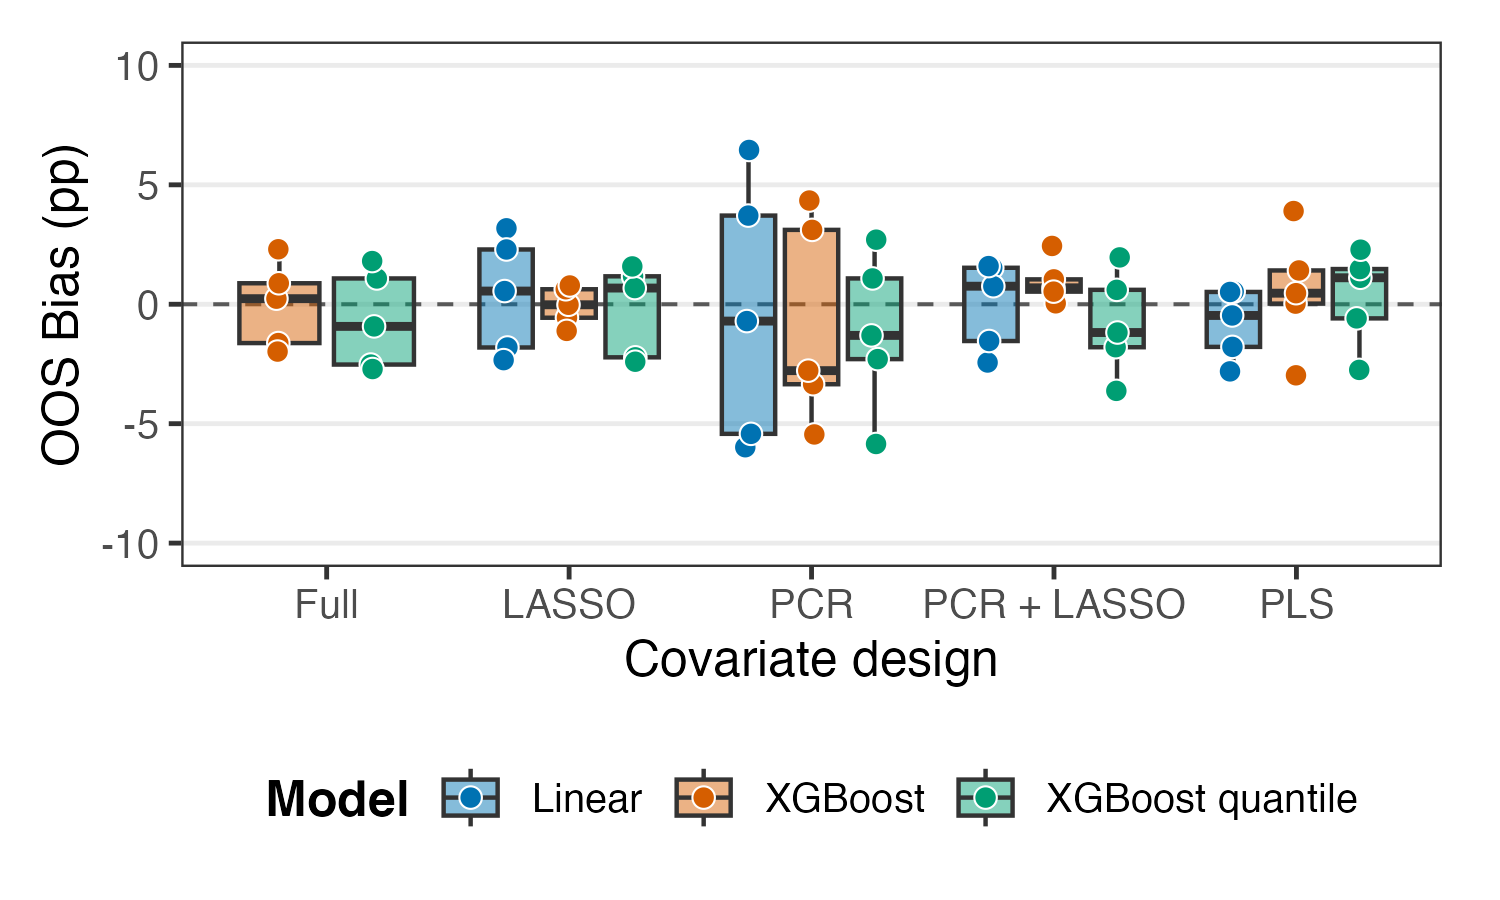
\includegraphics[width=.45\linewidth]{Fig4c_error.png}
        \caption{Data scenario (3): Baseline with mobility factor}
        \label{fig:OOS-baseline-mobile-pca-mean}
    \end{subfigure}

    \medskip
    \begin{subfigure}[t]{\textwidth}
        \centering
        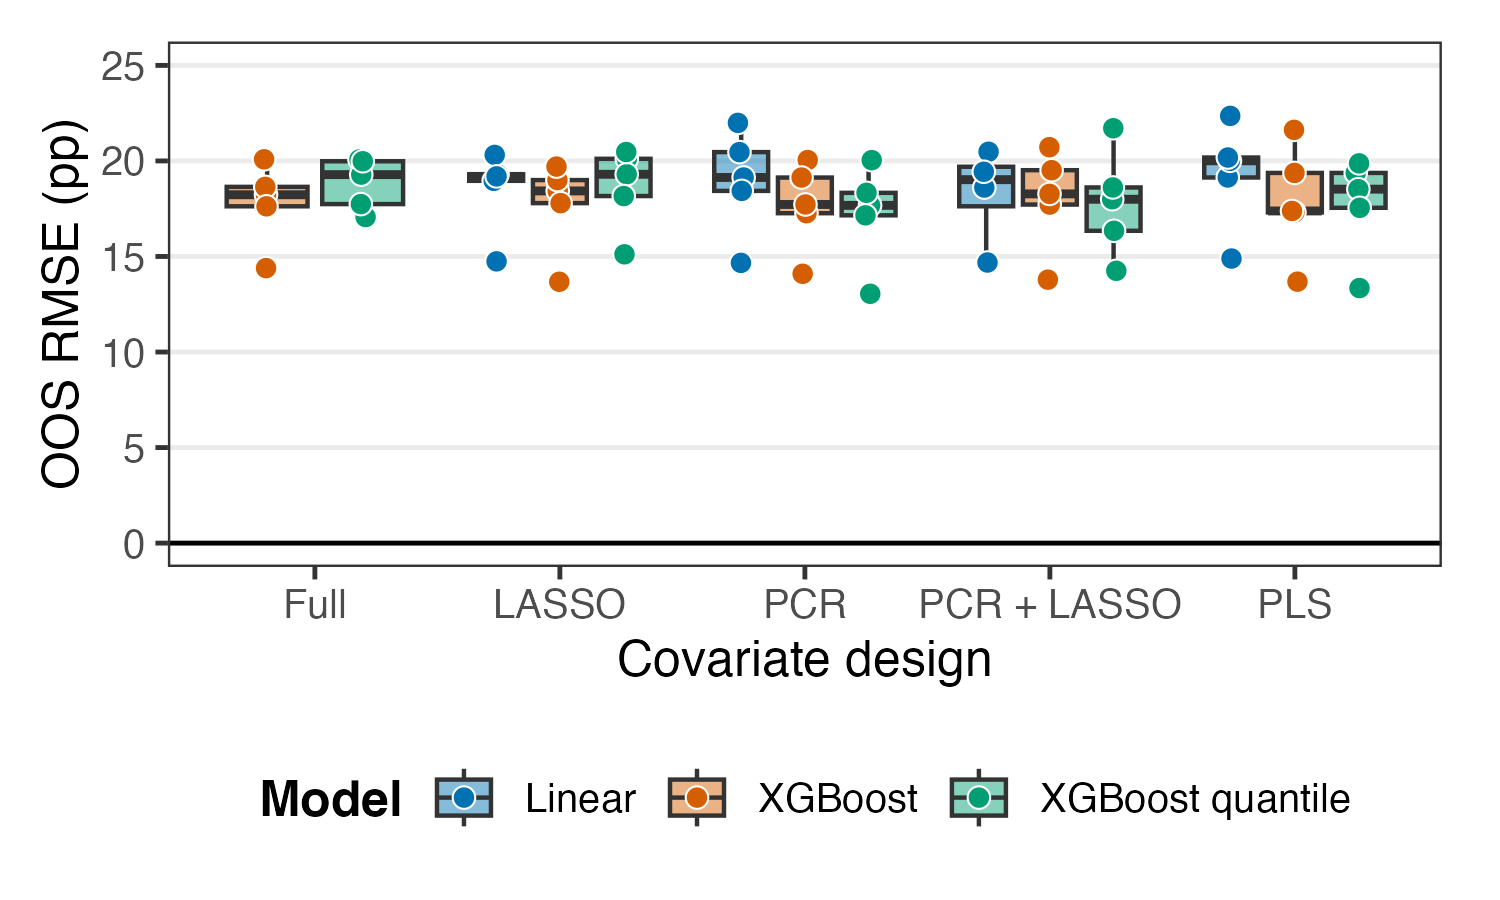
\includegraphics[width=.45\linewidth]{Fig4d_rmse.png}
        \hspace{0.03\linewidth}
        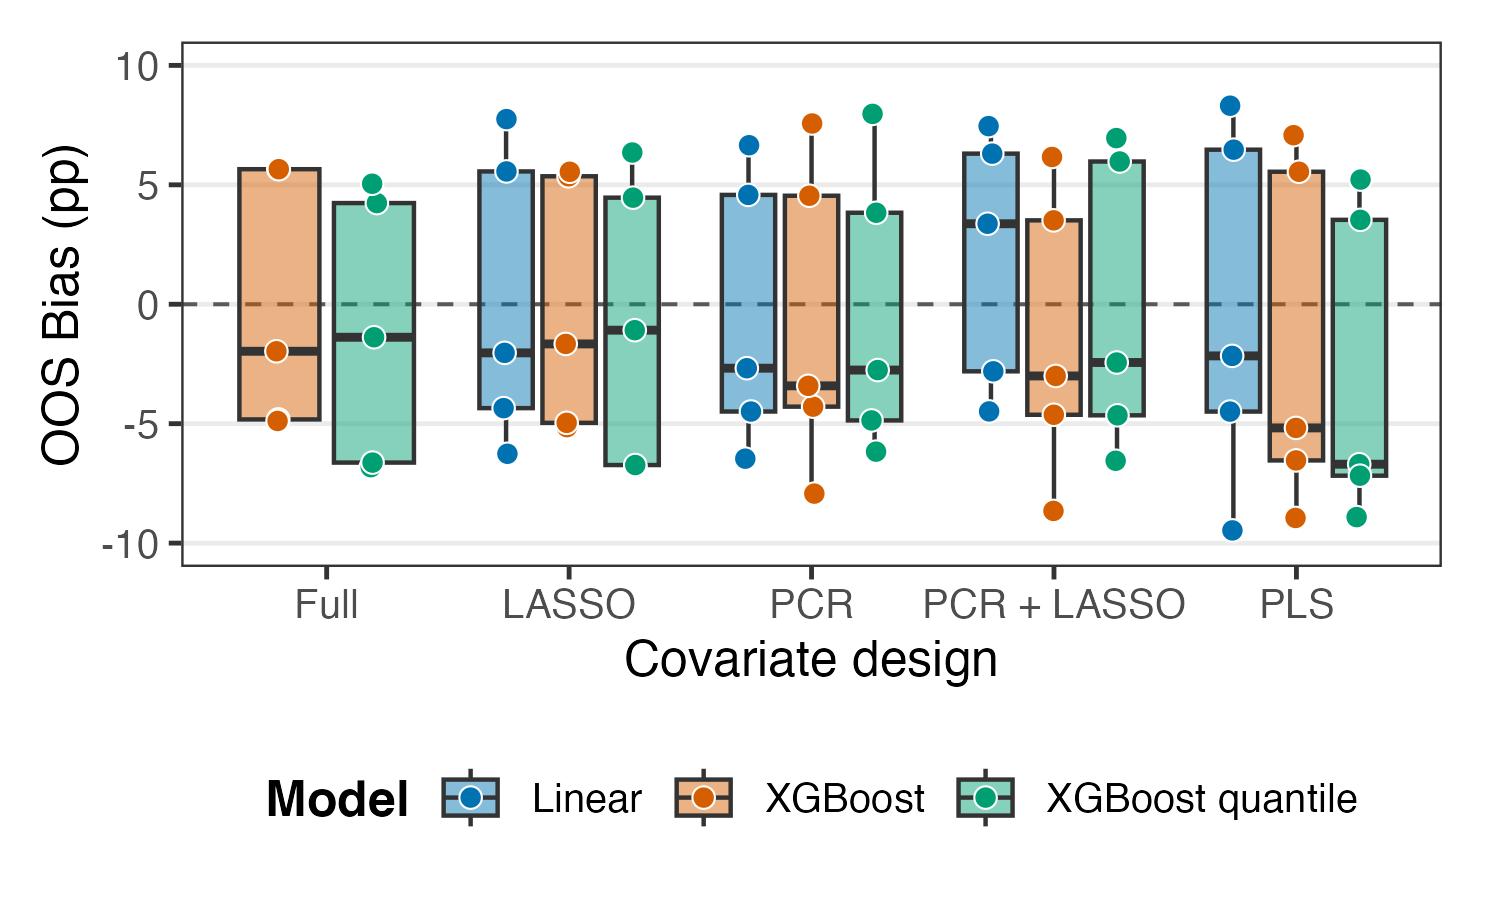
\includegraphics[width=.45\linewidth]{Fig4d_error.png}
        \caption{Data scenario (4): Mobility data}
        \label{fig:OOS-mobile-only-mean}
    \end{subfigure}

    \caption{Out-of-sample RMSE (left) and signed error (right) across spatial folds, models, and covariate designs}
    \label{fig:OOS-performance-scenarios}
\end{figure}


\subsection{Prediction Errors across Poverty Levels}

Because XGBoost is among the best-performing models in the OOS evaluation, we use it for the distributional analysis. Figure~\ref{fig:distributional-bias-xgboost} reports population-weighted local regression estimates of the conditional OOS signed error for XGBoost across true canton poverty rates, covariate designs, and data scenarios. Positive values indicate overprediction and negative values indicate underprediction.

First, specifications containing administrative covariates exhibit the most favorable distributional performance. The full and LASSO designs remain closest to zero across most of the poverty distribution and show comparatively smaller deviations in the tails. In the leading administrative specification, absolute signed error at the endpoints of the local curves is approximately 10 percentage points. The curves remain similar when mobility indicators are added directly or through their first principal component. Mobility-only models retain information about the overall level of poverty, but their weaker average accuracy is accompanied by larger distortions across the distribution.

Second, the predictions compress observed geographic differences: they tend to exceed census poverty in low-poverty cantons and fall below it in high-poverty cantons. Part of this pattern is expected, since a conditional-mean prediction is less dispersed than observed outcomes whenever residual variation is present; when errors are conditioned on the realized outcome, this mechanically produces positive errors at the low end and negative errors at the high end \citep{Hastie2009}. Compression in these curves therefore does not by itself establish misspecification or miscalibration conditional on the predictions. Its policy relevance is nonetheless direct: a small net error across cantons does not ensure small errors in the most deprived territories, even under the best-performing specifications.

This pattern matches the direction documented by \citet{Corral2025}, who find overprediction in less deprived and underprediction in more deprived areas, increasing toward the tails, despite good average performance. \citet{CorralRodas2025Aggregation} show, through a different mechanism, that matching average welfare does not ensure accurate poverty rates when models fail to reproduce within-area variation. Although our direct canton-level predictions involve a different estimand, all three results indicate that strong average fit does not guarantee accurate predictions across the poverty distribution. In our application, the full and LASSO administrative designs provide the strongest combination of aggregate accuracy, spatial stability, and distributional performance.


\begin{figure}[!htbp]
    \centering

    \begin{subfigure}[t]{0.49\textwidth}
        \centering
        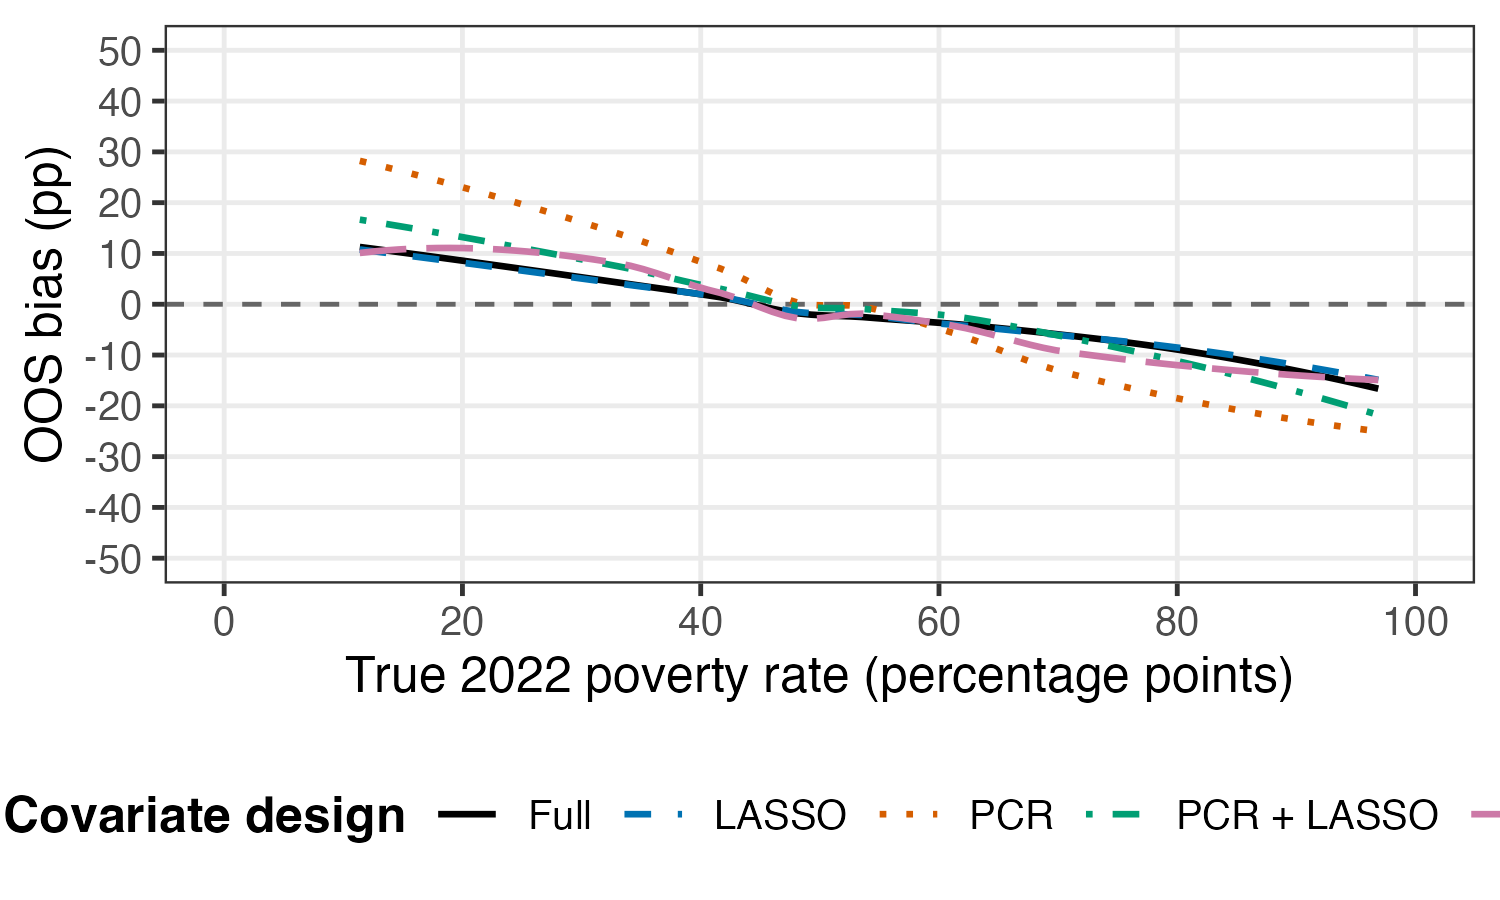
\includegraphics[width=\linewidth]
        {Fig5a.png}
        \caption{Data scenario (1): Baseline}
        \label{fig:distributional-bias-baseline}
    \end{subfigure}
    \hfill
    \begin{subfigure}[t]{0.49\textwidth}
        \centering
        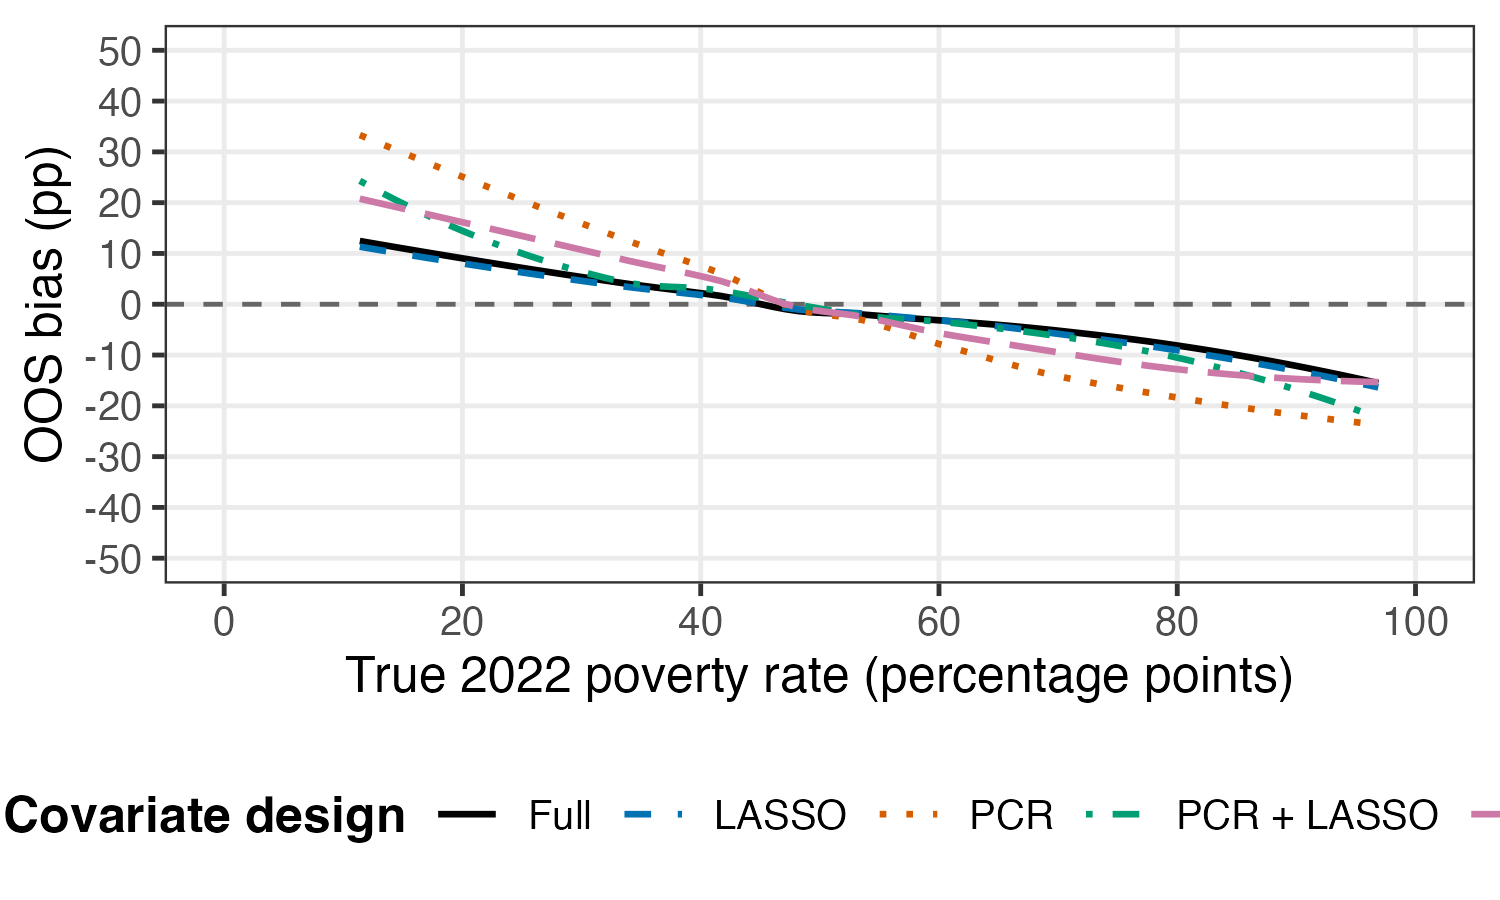
\includegraphics[width=\linewidth]
        {Fig5b.png}
        \caption{Data scenario (2): Baseline with mobility data}
        \label{fig:distributional-bias-mobile-mean}
    \end{subfigure}

    \medskip
    \begin{subfigure}[t]{0.49\textwidth}
        \centering
        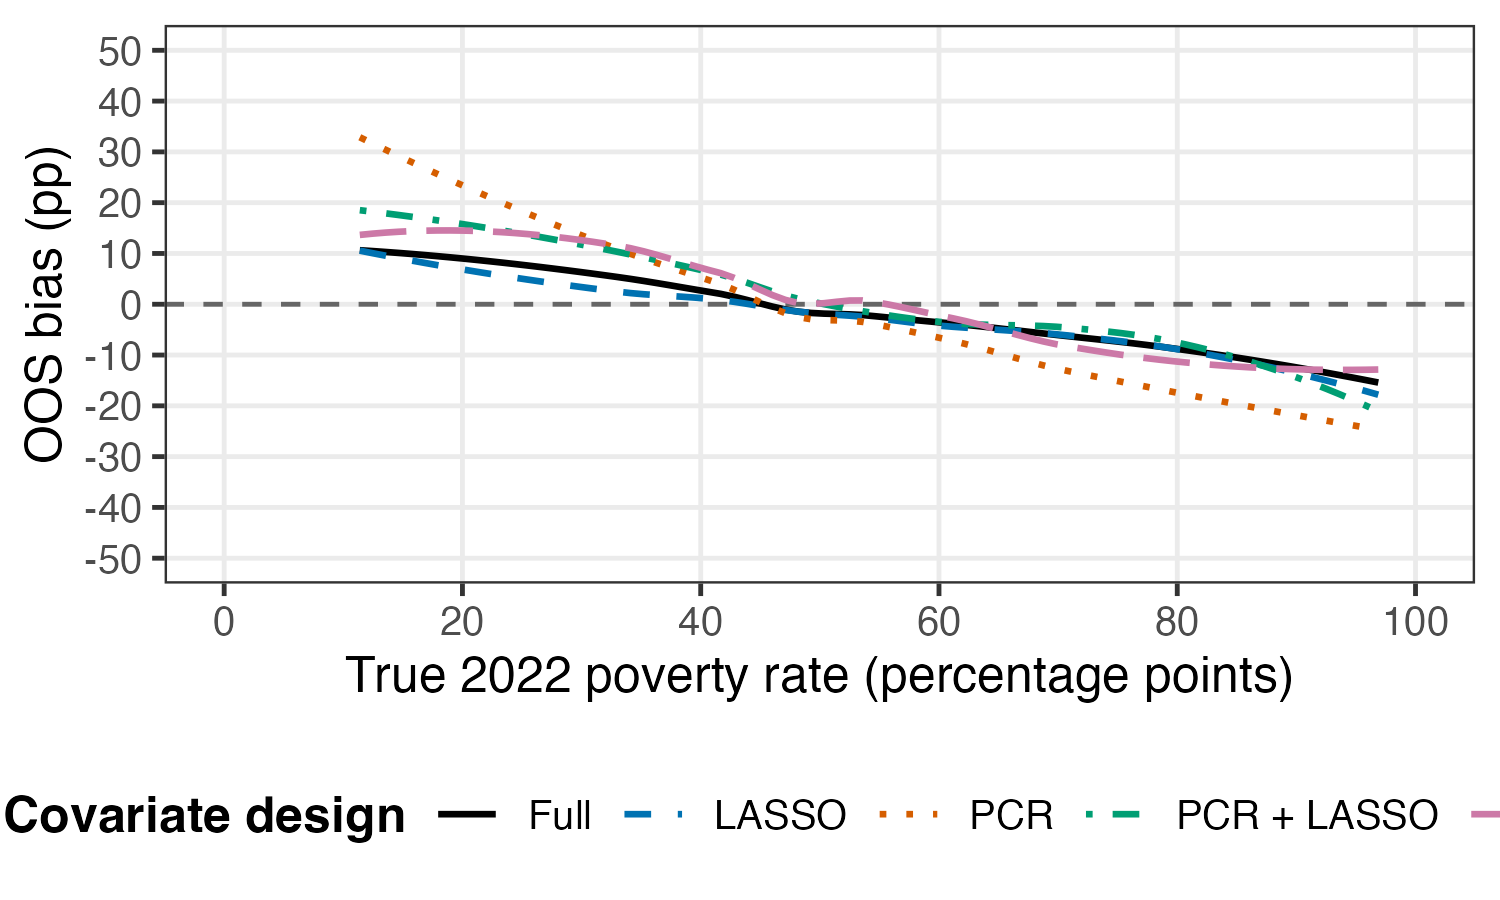
\includegraphics[width=\linewidth]
        {Fig5c.png}
        \caption{Data scenario (3): Baseline with mobility factor}
        \label{fig:distributional-bias-mobile-pca-mean}
    \end{subfigure}
    \hfill
    \begin{subfigure}[t]{0.49\textwidth}
        \centering
        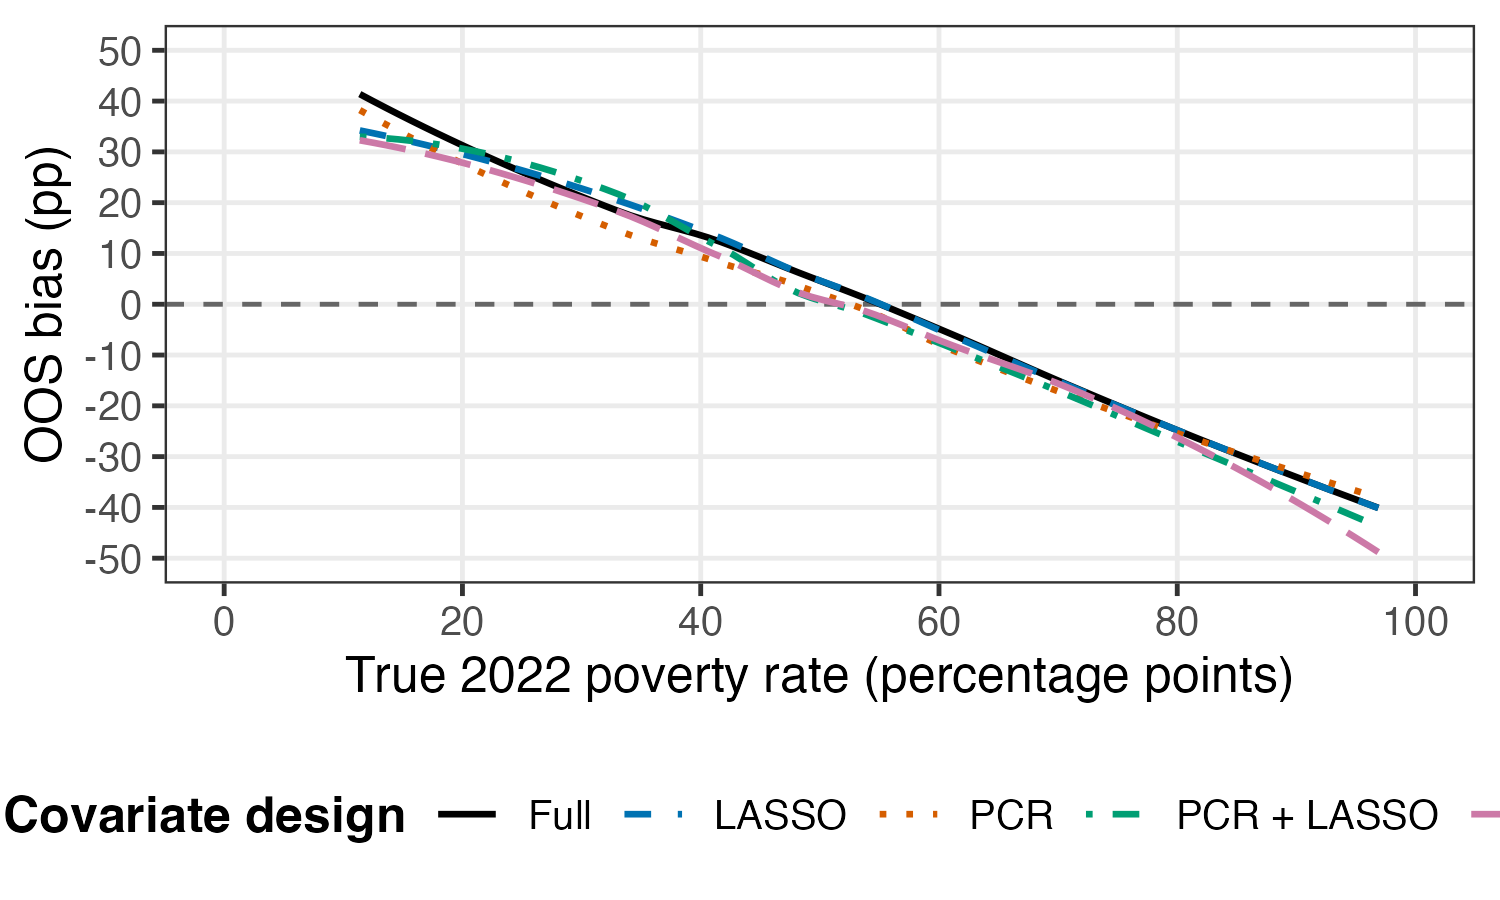
\includegraphics[width=\linewidth]
        {Fig5d.png}
        \caption{Data scenario (4): Mobility data}
        \label{fig:distributional-bias-mobile-only-mean}
    \end{subfigure}

    \caption{Population-weighted LOESS estimates of the conditional out-of-sample signed prediction error for XGBoost, by true canton poverty rate and covariate design. Positive values indicate overprediction and negative values indicate underprediction}
    \label{fig:distributional-bias-xgboost}
\end{figure}


\subsection{Which Covariates Drive Prediction?}
\label{sec:covariate_importance}

To describe the variables driving the leading specification, we compute exact TreeSHAP values for XGBoost under the full covariate design in each data scenario \citep{Lundberg2017}. SHAP values are calculated for the final model refitted on all 218 cantons after hyperparameter selection through spatial cross-validation, so this analysis describes the fitted prediction function rather than an independent spatial evaluation. For each variable, global importance is defined as the mean absolute SHAP value across cantons, measuring the average magnitude of its contribution to fitted predictions. Appendix~\ref{app:shap} reports the twenty variables with the largest mean absolute SHAP values, expressed in percentage points of predicted poverty.

First, administrative variables provide the strongest and most stable predictive signals. The same five variables occupy the leading positions in all three scenarios containing administrative covariates. School internet connectivity ranks first, with mean absolute SHAP values of 3.21--3.59 percentage points, followed by adolescent fertility (2.53--2.84) and ATM density (1.79--1.99). Financial-service access points (0.95--1.28) and GDP per capita (0.94--1.08) alternate between fourth and fifth place. This stable ordering shows that the fitted models consistently draw their strongest signals from education, health, financial access, and local economic activity. The prominence of connectivity echoes \citet{Corral2025}, whose feature analysis also places internet access among the leading predictors, although the variables and attribution methods differ.

Second, mobility indicators provide little additional signal when administrative covariates are available: no mobility indicator enters the twenty most important variables in any scenario containing official covariates. Together with the accuracy comparison in Figure~\ref{fig:OOS-performance-scenarios}, this is consistent with official records already capturing much of the information contained in aggregated mobility. The attribution evidence alone cannot prove redundancy, because correlated predictors can share or redistribute attribution. SHAP rankings identify predictive contributions, not causal effects of the underlying variables.


\section{Robustness Checks}
\label{sec:robustness}

\subsection{Robustness I: Mobility under Staggered Data Availability}
\label{sec:staggered-availability}

The preceding analysis evaluates the predictive information in each set of covariates without regard to publication dates. Because mobility data are available promptly while administrative records are released through different institutional calendars, mobility could be more valuable when official information is limited. We examine this possibility by restricting the predictor set to a reduced group of leading indicators and expanding it according to their publication calendar (Table~\ref{tab:calendar}), so that the information set grows cumulatively from Q1 to Q4. At each stage, we estimate full-design XGBoost models with and without the first mobility principal component, constructed within each training fold.

This exercise is a stylized comparison of information sets rather than a real-time forecasting evaluation. The twenty administrative indicators are those with the largest SHAP values in the baseline model refitted on the full sample (Appendix~\ref{app:shap}), so the outcome informs their selection, and the outcome and mobility snapshot refer to 2022 and 2024 regardless of the quarter assigned to each predictor. Absolute accuracy at each stage may therefore be optimistic. The main object of interest is the paired comparison with and without mobility at a fixed stage, which uses identical administrative predictors and is less affected by this selection.


\begin{table}[!htbp]
    \centering
    \footnotesize
    \renewcommand{\arraystretch}{1.05}
    \begin{tabular}{p{0.72\textwidth}ccc}
        \toprule
        \textbf{Variable} & \textbf{Q1} & \textbf{Q2} & \textbf{Q4} \\ \midrule
        Percentage of Schools with Internet & X &  &  \\
        Fertility Rate (Ages 11--19, Mother) &  & X &  \\
        ATMs per Population (15+) &  & X &  \\
        GDP per Capita &  &  & X \\
        Financial Service Points per Population (15+) &  & X &  \\
        Prevalence of Hospital Discharges (Cholelithiasis K80) &  &  & X \\
        Prevalence of Musculoskeletal Diseases &  &  & X \\
        Public Education Institutions & X &  &  \\
        Sales Share: Mining and Quarrying & X &  &  \\
        Average Prenatal Checkups &  & X &  \\
        Total Fertility Rate (Mother) &  & X &  \\
        GDP Share of Education &  &  & X \\
        Cooperative Accounts (Men) per Population (15+) &  & X &  \\
        Promotion Rate, Third Year EGB (Male) & X &  &  \\
        Education Institutions & X &  &  \\
        Access to Drinking Water (Households) &  &  & X \\
        Moderate Preterm Birth Rate (Female) &  & X &  \\
        Prevalence of Congenital Malformations &  &  & X \\
        General Fertility Rate &  & X &  \\
        Public Bank Current Accounts &  & X &  \\
        Mobility Factor (PCA Mean) & X &  &  \\
        \midrule
        \textbf{Total (new variables)} & 6 & 9 & 6   \\
        \textbf{Cumulative} & 6 & 15 & 21 \\
        \bottomrule
    \end{tabular}
    \caption{Publication Calendar of the Selected Administrative Indicators and Mobility Factor. An X indicates the quarter in which each variable becomes available. Counts include the mobility factor; models without mobility use the same administrative indicators and exclude the factor}
    \label{tab:calendar}
\end{table}


Figure~\ref{fig:distributional_calendar_a} shows that predictive accuracy improves markedly as administrative information accumulates from Q1 to Q4. The dispersion of results across spatial folds also declines, indicating that performance becomes more stable across excluded regions as the information set expands. Mobility has little effect on Q1 RMSE and produces only modest changes in fold-level signed error, and its incremental contribution remains limited as additional administrative data enter. Figure~\ref{fig:distributional_calendar_b} shows that signed errors in the tails generally decline as the information set expands and change little when mobility data are added. Across both figures, the main gains in accuracy and stability accompany the expanding administrative information set rather than the promptly available mobility factor. Because indicators enter jointly by stage, these gains cannot be attributed to a particular variable or domain, nor interpreted as the effect of accelerating any specific release.


\begin{figure}[!htbp]
    \centering
    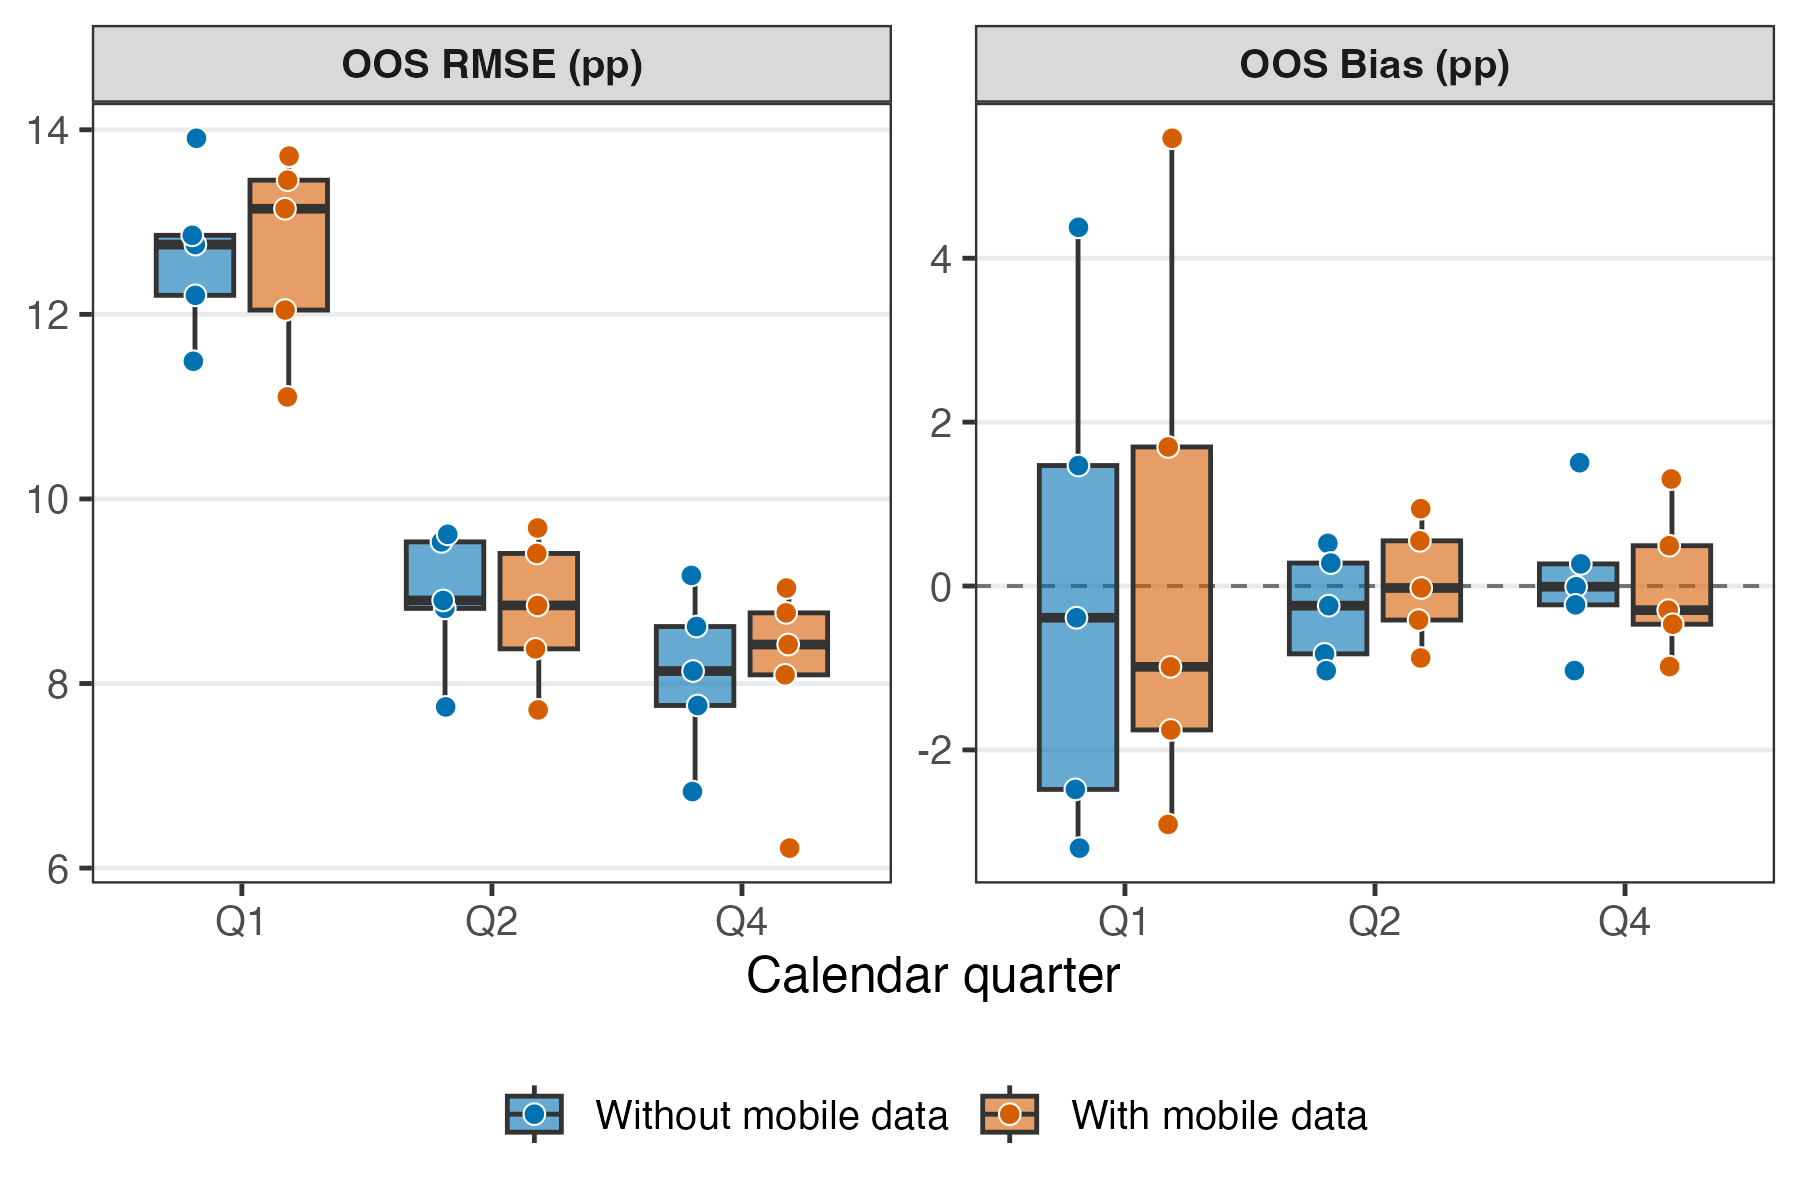
\includegraphics[width=0.7\linewidth]{Fig6.png}
    \caption{Out-of-sample performance under cumulative calendar information. The left panel reports RMSE in percentage points; the right panel reports fold-level mean signed error, defined as $100\times(\widehat{y}-y)$, so positive values indicate overprediction and negative values indicate underprediction. Boxes summarize the five outer spatial folds for full-design XGBoost models with and without the first mobility principal component; points identify folds. Q1, Q2, and Q4 denote the cumulative administrative information available by each quarter}
    \label{fig:distributional_calendar_a}
\end{figure}


\begin{figure}[!htbp]
    \centering
    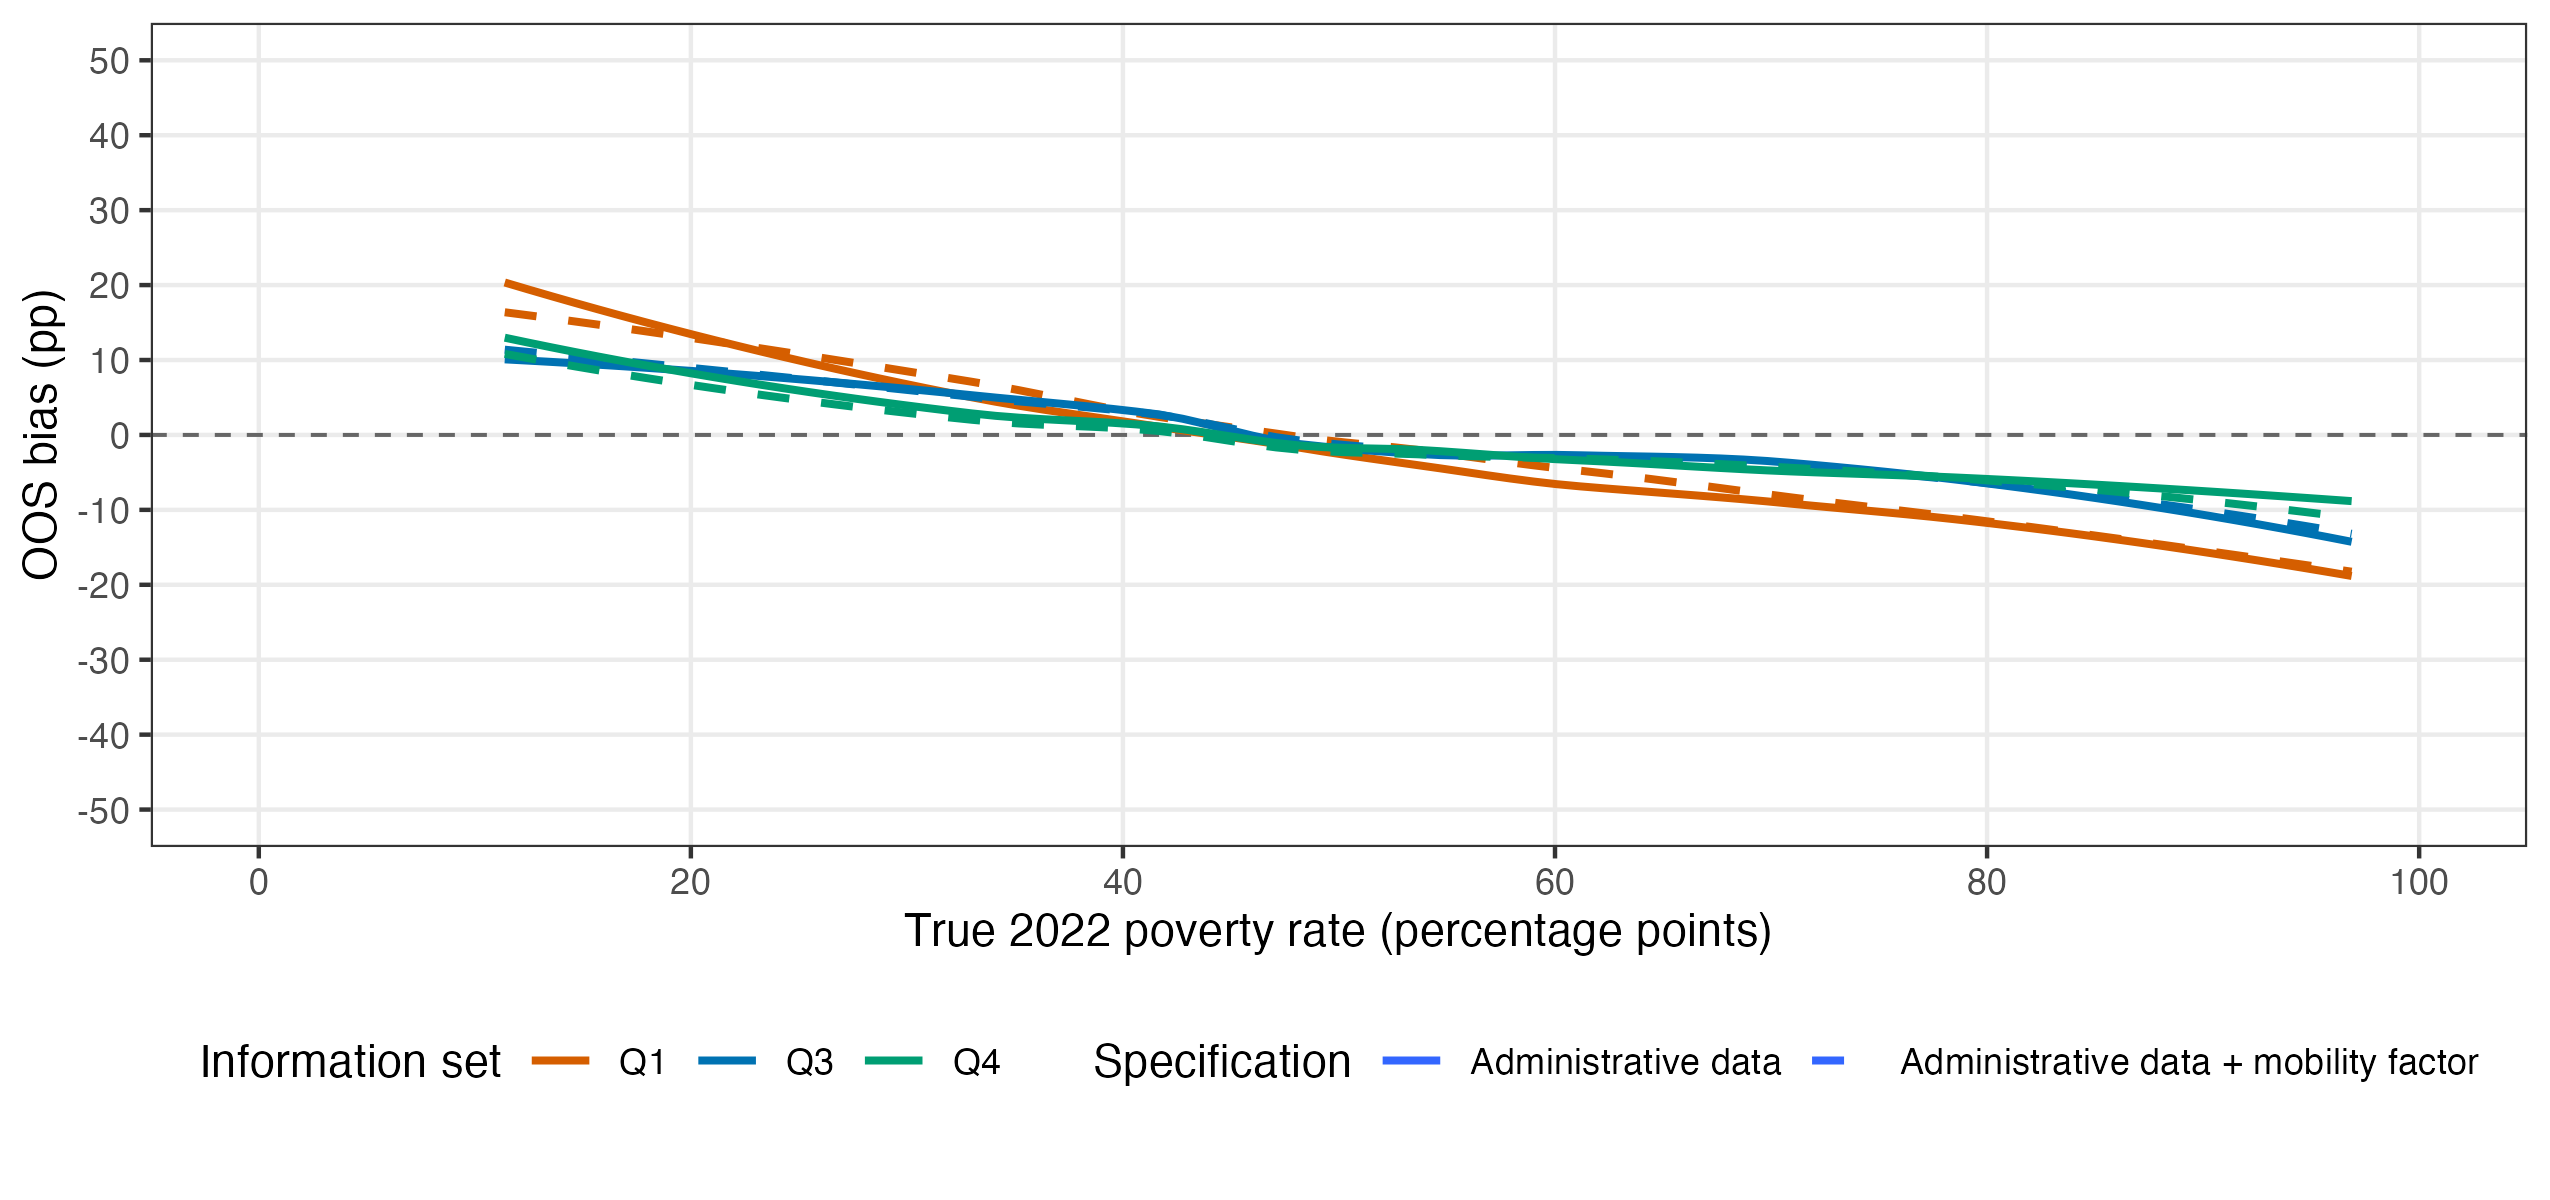
\includegraphics[width=0.7\linewidth]{Fig7.png}
    \caption{Population-weighted LOESS estimates of conditional out-of-sample prediction error for the full-design XGBoost model, by true canton poverty rate and calendar information set, with and without the mobility factor. Positive values indicate overprediction, and negative values indicate underprediction}
    \label{fig:distributional_calendar_b}
\end{figure}

\subsection{Robustness II: Sensitivity to Alternative Spatial Partitions}
\label{subsec:repeated_cv}

Appendix~\ref{app:repeated_spatial_cv} examines whether the main comparison depends on the particular spatial partition (Table~\ref{tab:repeated-spatial-cv}). Across ten repetitions with different clustering seeds, the administrative-only full XGBoost specification achieves an average OOS RMSE of 9.44 percentage points. Adding the mobility factor increases RMSE by 0.06 points on average, while including the 38 mobility indicators increases it by 0.02 points. The empirical 2.5th--97.5th percentile ranges of the paired differences are narrow and straddle zero: $[-0.16, 0.26]$ for the mobility factor and $[-0.22, 0.24]$ for the 38 indicators. Both lie within $\pm 0.50$ percentage points, a margin small relative to the leading RMSE of roughly 9.4 points.

These ranges measure sensitivity to partition choice; they are not population-sampling confidence intervals or a formal equivalence test. Their contribution is to show that the central comparison does not hinge on one geographic split: under the full administrative information set, mobility produces neither a systematic nor a large improvement in accuracy across the tested partitions. This should not be read as evidence that mobility contains no predictive information, but rather that its incremental contribution is negligible once the complete administrative covariate set is available.


\section{Conclusion}
\label{sec:conclusion}

This paper evaluates mobile phone mobility indicators against a very rich official benchmark: 947 administrative predictors for 218 mainland cantons. Nested spatial cross-validation keeps all transformations and hyperparameter tuning within the training territories and produces geographically OOS predictions for every canton. Administrative specifications achieve the strongest predictive performance, with spatial RMSEs of roughly 9.4 to 9.6 percentage points for the leading designs. Adding mobility indicators, either directly or through their first principal component, produces no detectable improvement in average accuracy under the evaluated models and evaluation scheme. This result holds across ten alternative spatial partitions, where the paired difference in RMSE remains within a fraction of a percentage point.

This result does not imply that mobility contains no socioeconomic information. Mobility-only models retain predictive signal, although with errors roughly twice as large as those of the leading administrative specifications. The staggered-calendar exercise points in the same direction. Accuracy improves and variation across spatial folds declines as administrative information accumulates, while performance with and without the mobility factor remains similar at each stage. The most informative signals come from education, health, financial access, and local economic activity, with school internet connectivity, adolescent fertility, and ATM density consistently leading the fitted models. The value of a non-traditional data source is therefore not intrinsic. It depends on the official information already available for the outcome being predicted.

The OOS predictions also compress the observed poverty distribution, tending to overpredict poverty in relatively low-poverty cantons and underpredict it in high-poverty cantons. This pattern describes errors conditional on observed deprivation. It is not an estimate of repeated-sampling bias or of fiscal or welfare consequences. It nonetheless shows that favorable aggregate accuracy can coexist with a systematic understatement of the differences that motivate territorial measurement. The pattern is consistent with \citet{Corral2025}, and \citet{CorralRodas2025Aggregation} reinforce the broader conclusion that good average fit does not ensure accuracy across the poverty distribution.

These findings have several implications for policy and for the organization of statistical information.

First, investment in administrative information systems should be a priority for intercensal poverty monitoring. Records that public institutions already collect in the course of their operations jointly predict structural deprivation with considerable accuracy in territories excluded from estimation. Their value comes from integration across domains rather than from any single source. This suggests that the marginal return to strengthening and connecting existing registries may be high relative to acquiring new data. Statistical agencies such as INEC can build on this by consolidating administrative indicators into a standing canton-level predictor system. Such a system would require shared geographic identifiers, consistent indicator definitions over time, explicit population denominators, and documented publication calendars. A record of revisions would help distinguish newly released observations from corrections to earlier releases. These steps are consistent with the emphasis on combining and reusing data for development in \citet{WorldBank2021Data}.

Second, timeliness of administrative releases deserves attention alongside coverage and quality. The calendar exercise shows that useful predictive information is available before the full set of selected indicators is published, and that each subsequent release improves accuracy and stability across territories. Agencies can therefore produce provisional territorial diagnostics from the records released early in the year and update them as further information arrives, rather than waiting for complete annual compilations. Documenting reporting lags and improving the accessibility of early releases would make this sequential use of information more practical. The evidence identifies the value of the information sets, not the payoff from accelerating any particular release, so priorities for improving timeliness should also weigh collection processes and the reliability of early figures.

Third, decisions to acquire or partner for digital data products should be based on their incremental contribution, not their standalone predictive power. A mobility dataset that predicts poverty reasonably well on its own can add little once official records are available. Evaluations that compare a digital source only against an empty information set can therefore overstate its practical value. Procurement and partnership agreements should specify the measurement task, the outcome, and the official information already available when the product would be used. They should require evidence of improvement relative to that benchmark under geographically held-out evaluation. Mobility data may remain valuable in settings with weaker administrative systems, at finer geographic scales, for more transient welfare outcomes, or for purposes other than poverty mapping, such as monitoring shocks, displacement, or access to services. Their use should be justified by the specific gap they fill.

Fourth, predictive maps should not be used directly as inputs into fiscal allocation without distributional validation. UBN enters the criteria used to distribute resources to decentralized governments under COOTAD \citep{COOTAD2010}. Because predictions compress geographic differences, a map with good average accuracy could understate need in the most deprived cantons and overstate it in the least deprived. Under a formula-based allocation, this would shift resources away from the territories the criterion is meant to favor. Before any predicted indicator informs allocation or geographic targeting, it should be assessed against the specific thresholds, rankings, and weights used by the relevant rule, with particular attention to the most deprived territories. Where predictions are used between censuses, recalibration methods that restore the dispersion of the observed distribution, together with periodic benchmarking against census and survey measures, should accompany their use. Predictive maps are best treated as complements to official measurement, informing planning and diagnostics, rather than as substitutes for the census in binding allocation decisions.

Fifth, the evaluation standards applied to poverty prediction should reflect its intended use. Random cross-validation and in-sample fit can substantially overstate accuracy when neighboring territories share conditions. Our results show spatial OOS errors several times larger than training errors. Agencies and researchers producing poverty maps should report geographically held-out performance and errors across the poverty distribution, not only average accuracy. They should also compare any new data source against the strongest available official benchmark. Adopting these standards would make it easier for users to judge whether a predicted map is fit for a given policy purpose.

Finally, the lessons extend beyond Ecuador. Many middle-income countries in Latin America and elsewhere have developed extensive administrative records in education, health, financial inclusion, and economic activity. They also face growing offers of alternative data from telecommunications operators and private platforms. The Ecuadorian evidence suggests that, for structural deprivation, the first step is to make full use of the public information these countries already produce. Digital sources should then be evaluated at the margin, for the specific outcomes and stages where official information is limited. Combining integrated administrative records, direct census and survey measurement, and careful assessment of new data sources offers a foundation for territorial poverty information that is timely, accurate, and appropriate to the decisions it is meant to support.

\section*{Data and code availability}
The data and analysis code supporting the findings are available from the corresponding author upon request. The Telef\'{o}nica mobile phone data are private and are not publicly available.

\section*{Supplementary information}
Online Resource 1 provides the complete variable dictionary, including the area, source, and name of each of the 985 predictors. Online Resource 2 reports the comparison of in-sample and spatial out-of-sample performance and hyperparameter tuning strategies.

\bibliography{ref}

\par\bigskip
\newcounter{mainfigures}
\newcounter{maintables}
\setcounter{mainfigures}{\value{figure}}
\setcounter{maintables}{\value{table}}
\begin{appendices}
\setcounter{figure}{\value{mainfigures}}
\setcounter{table}{\value{maintables}}
\renewcommand{\thefigure}{\arabic{figure}}
\renewcommand{\thetable}{\arabic{table}}

\section{Mobility Data: Construction and Descriptive Properties}
\label{app:Mobility}

As described in Section~\ref{sec:data}, we construct canton-level mobility indicators from the average internal and national traffic flows assigned to each canton. We consider two alternative representations: the complete set of 38 mean-based mobility indicators (Scenarios 2 and 4), and their first principal component (Scenario 3). In the descriptive analysis of the complete sample, the first component explains 96 percent of the total variance of the mobility indicators. This share concerns variation in mobility, not in poverty. The factor used in the spatial prediction exercises is re-estimated within each training sample.

The mean-based mobility indicators exhibit a weak positive relationship with poverty rates, as shown in Figure~\ref{fig:corr}. The mobility variables are also strongly correlated with one another, which motivates a principal component summary of their common information. These descriptive relationships do not establish that the mobility factor contains information beyond the administrative records.

Figure~\ref{fig:scree} presents the scree plot for the mean-based mobility indicators. The first principal component captures 96 percent of their total variance and retains the positive relationship with poverty, providing a parsimonious representation of their common variation. Its large variance share does not imply that later components contain no poverty-relevant information, which is why the full set of 38 indicators is also evaluated.

\begin{figure}[!htbp]
\centering
\begin{minipage}[t]{0.60\textwidth}
\vspace{0pt}
\centering
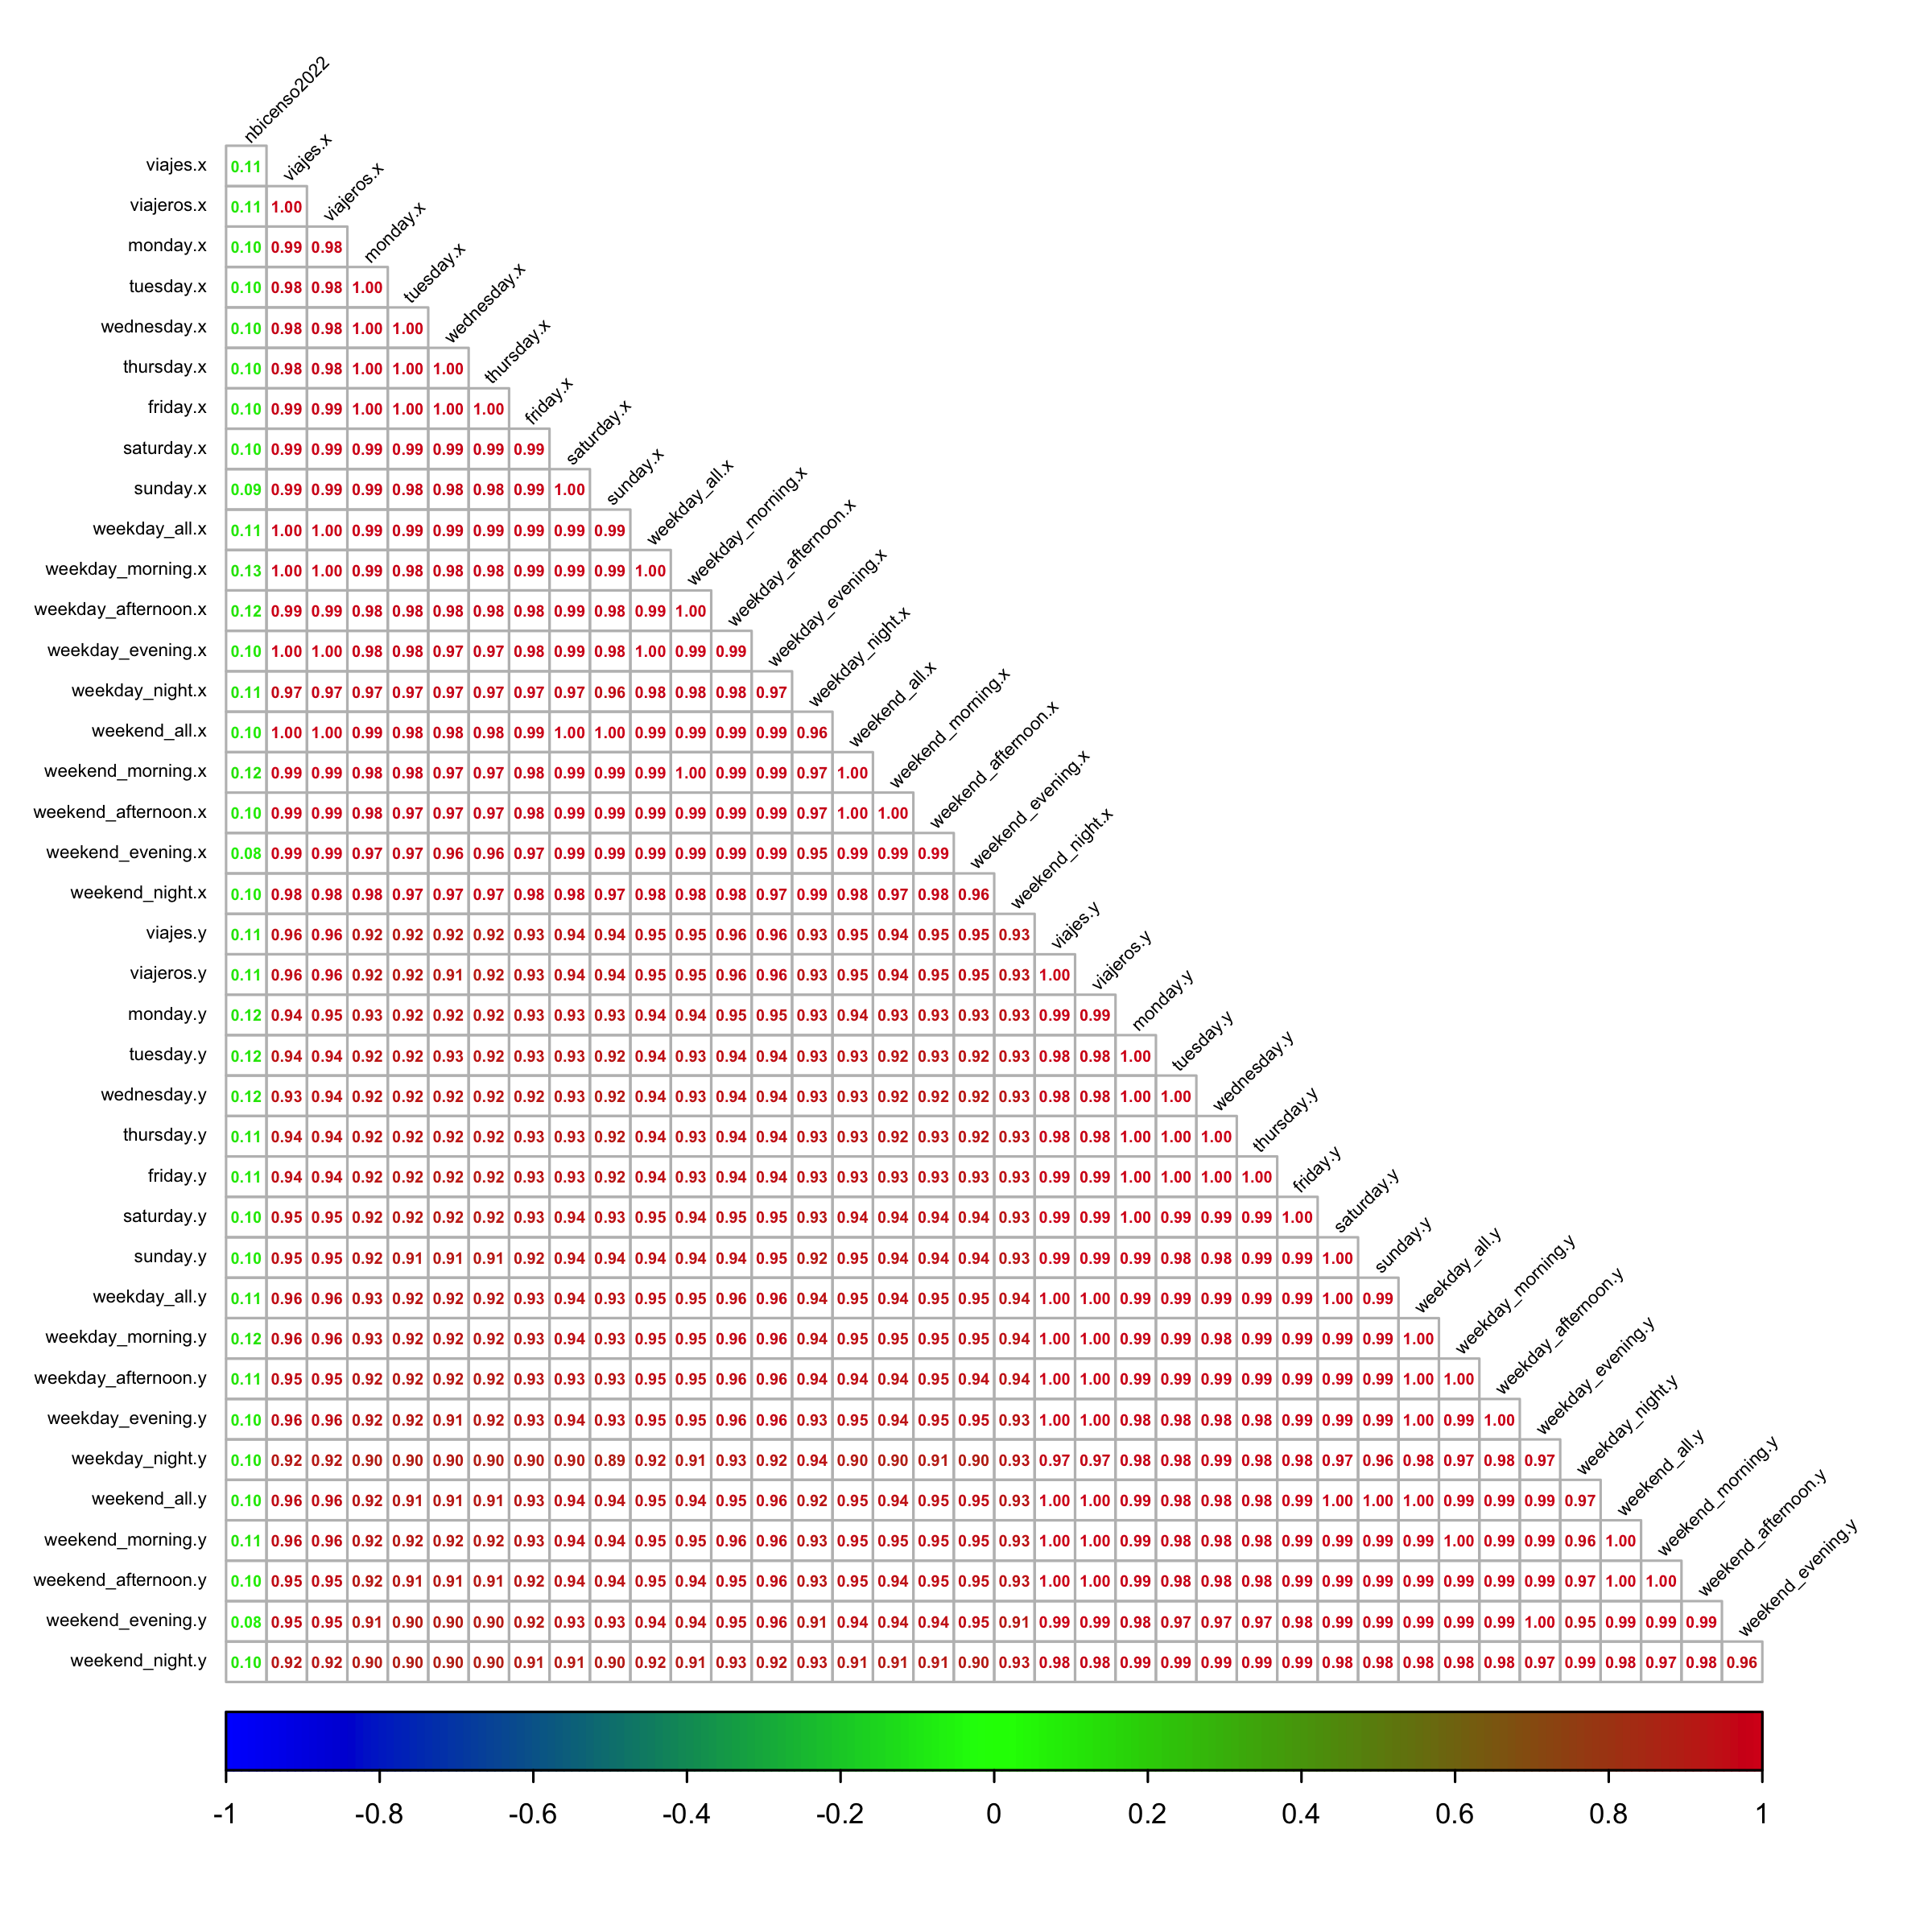
\includegraphics[width=\linewidth]{Fig8.png}
\caption{Correlation between mean-based mobility indicators and poverty rates}
\label{fig:corr}
\end{minipage}\hfill
\begin{minipage}[t]{0.38\textwidth}
\vspace{0pt}
\centering
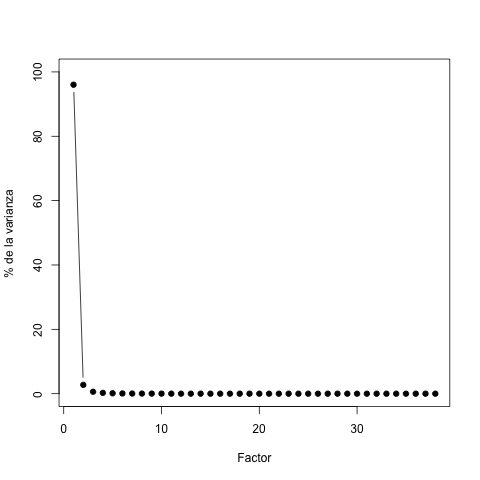
\includegraphics[width=\linewidth]{Fig9.png}
\caption{Scree plot for the mean-based mobility indicators}
\label{fig:scree}
\end{minipage}
\end{figure}

\clearpage
\section{Covariate Importance}
\label{app:shap}

Figure~\ref{fig:shap_scenarios} reports the twenty variables with the largest mean absolute SHAP values in each data scenario, as discussed in Section~\ref{sec:covariate_importance}.

\begin{figure}[!htbp]
\centering
\begin{subfigure}{0.90\textwidth}
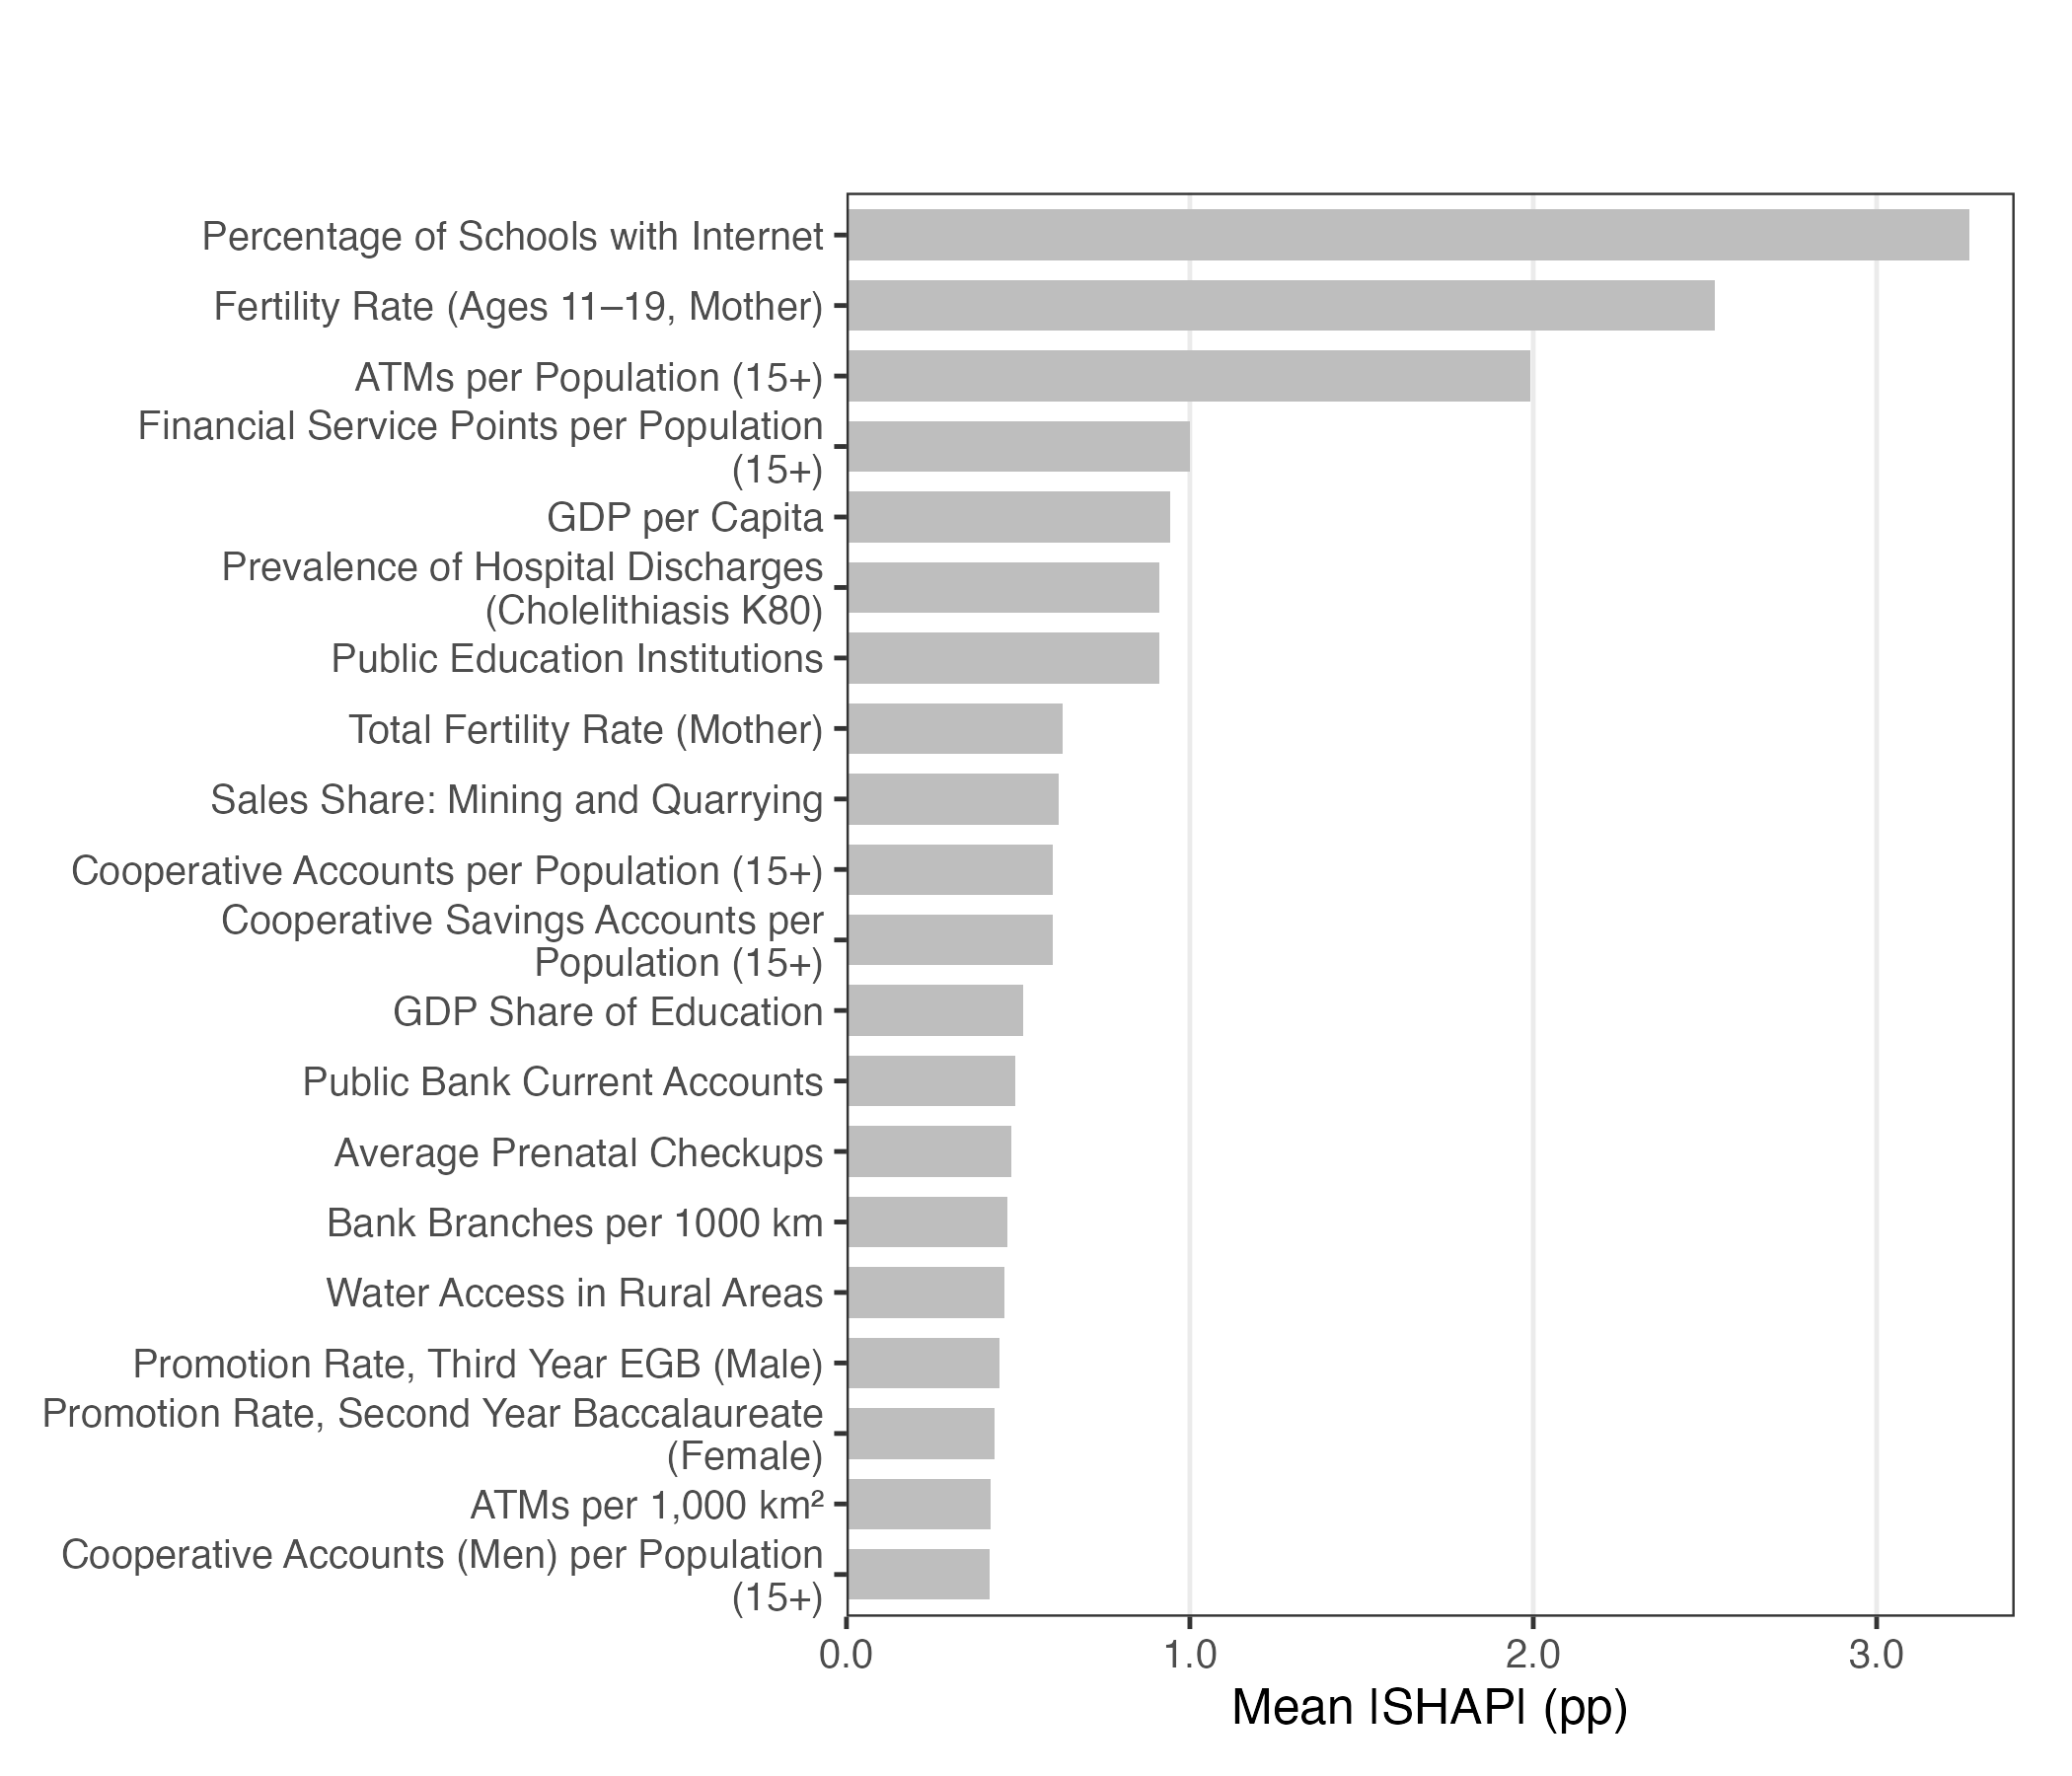
\includegraphics[width=\linewidth]{Fig10a.png}
\caption{Data scenario (1): Baseline}
\end{subfigure}
\caption{Top 20 covariates by mean absolute SHAP value (percentage points) for each scenario}
\label{fig:shap_scenarios}
\end{figure}

\begin{figure}[!htbp]
\ContinuedFloat
\centering
\begin{subfigure}{0.90\textwidth}
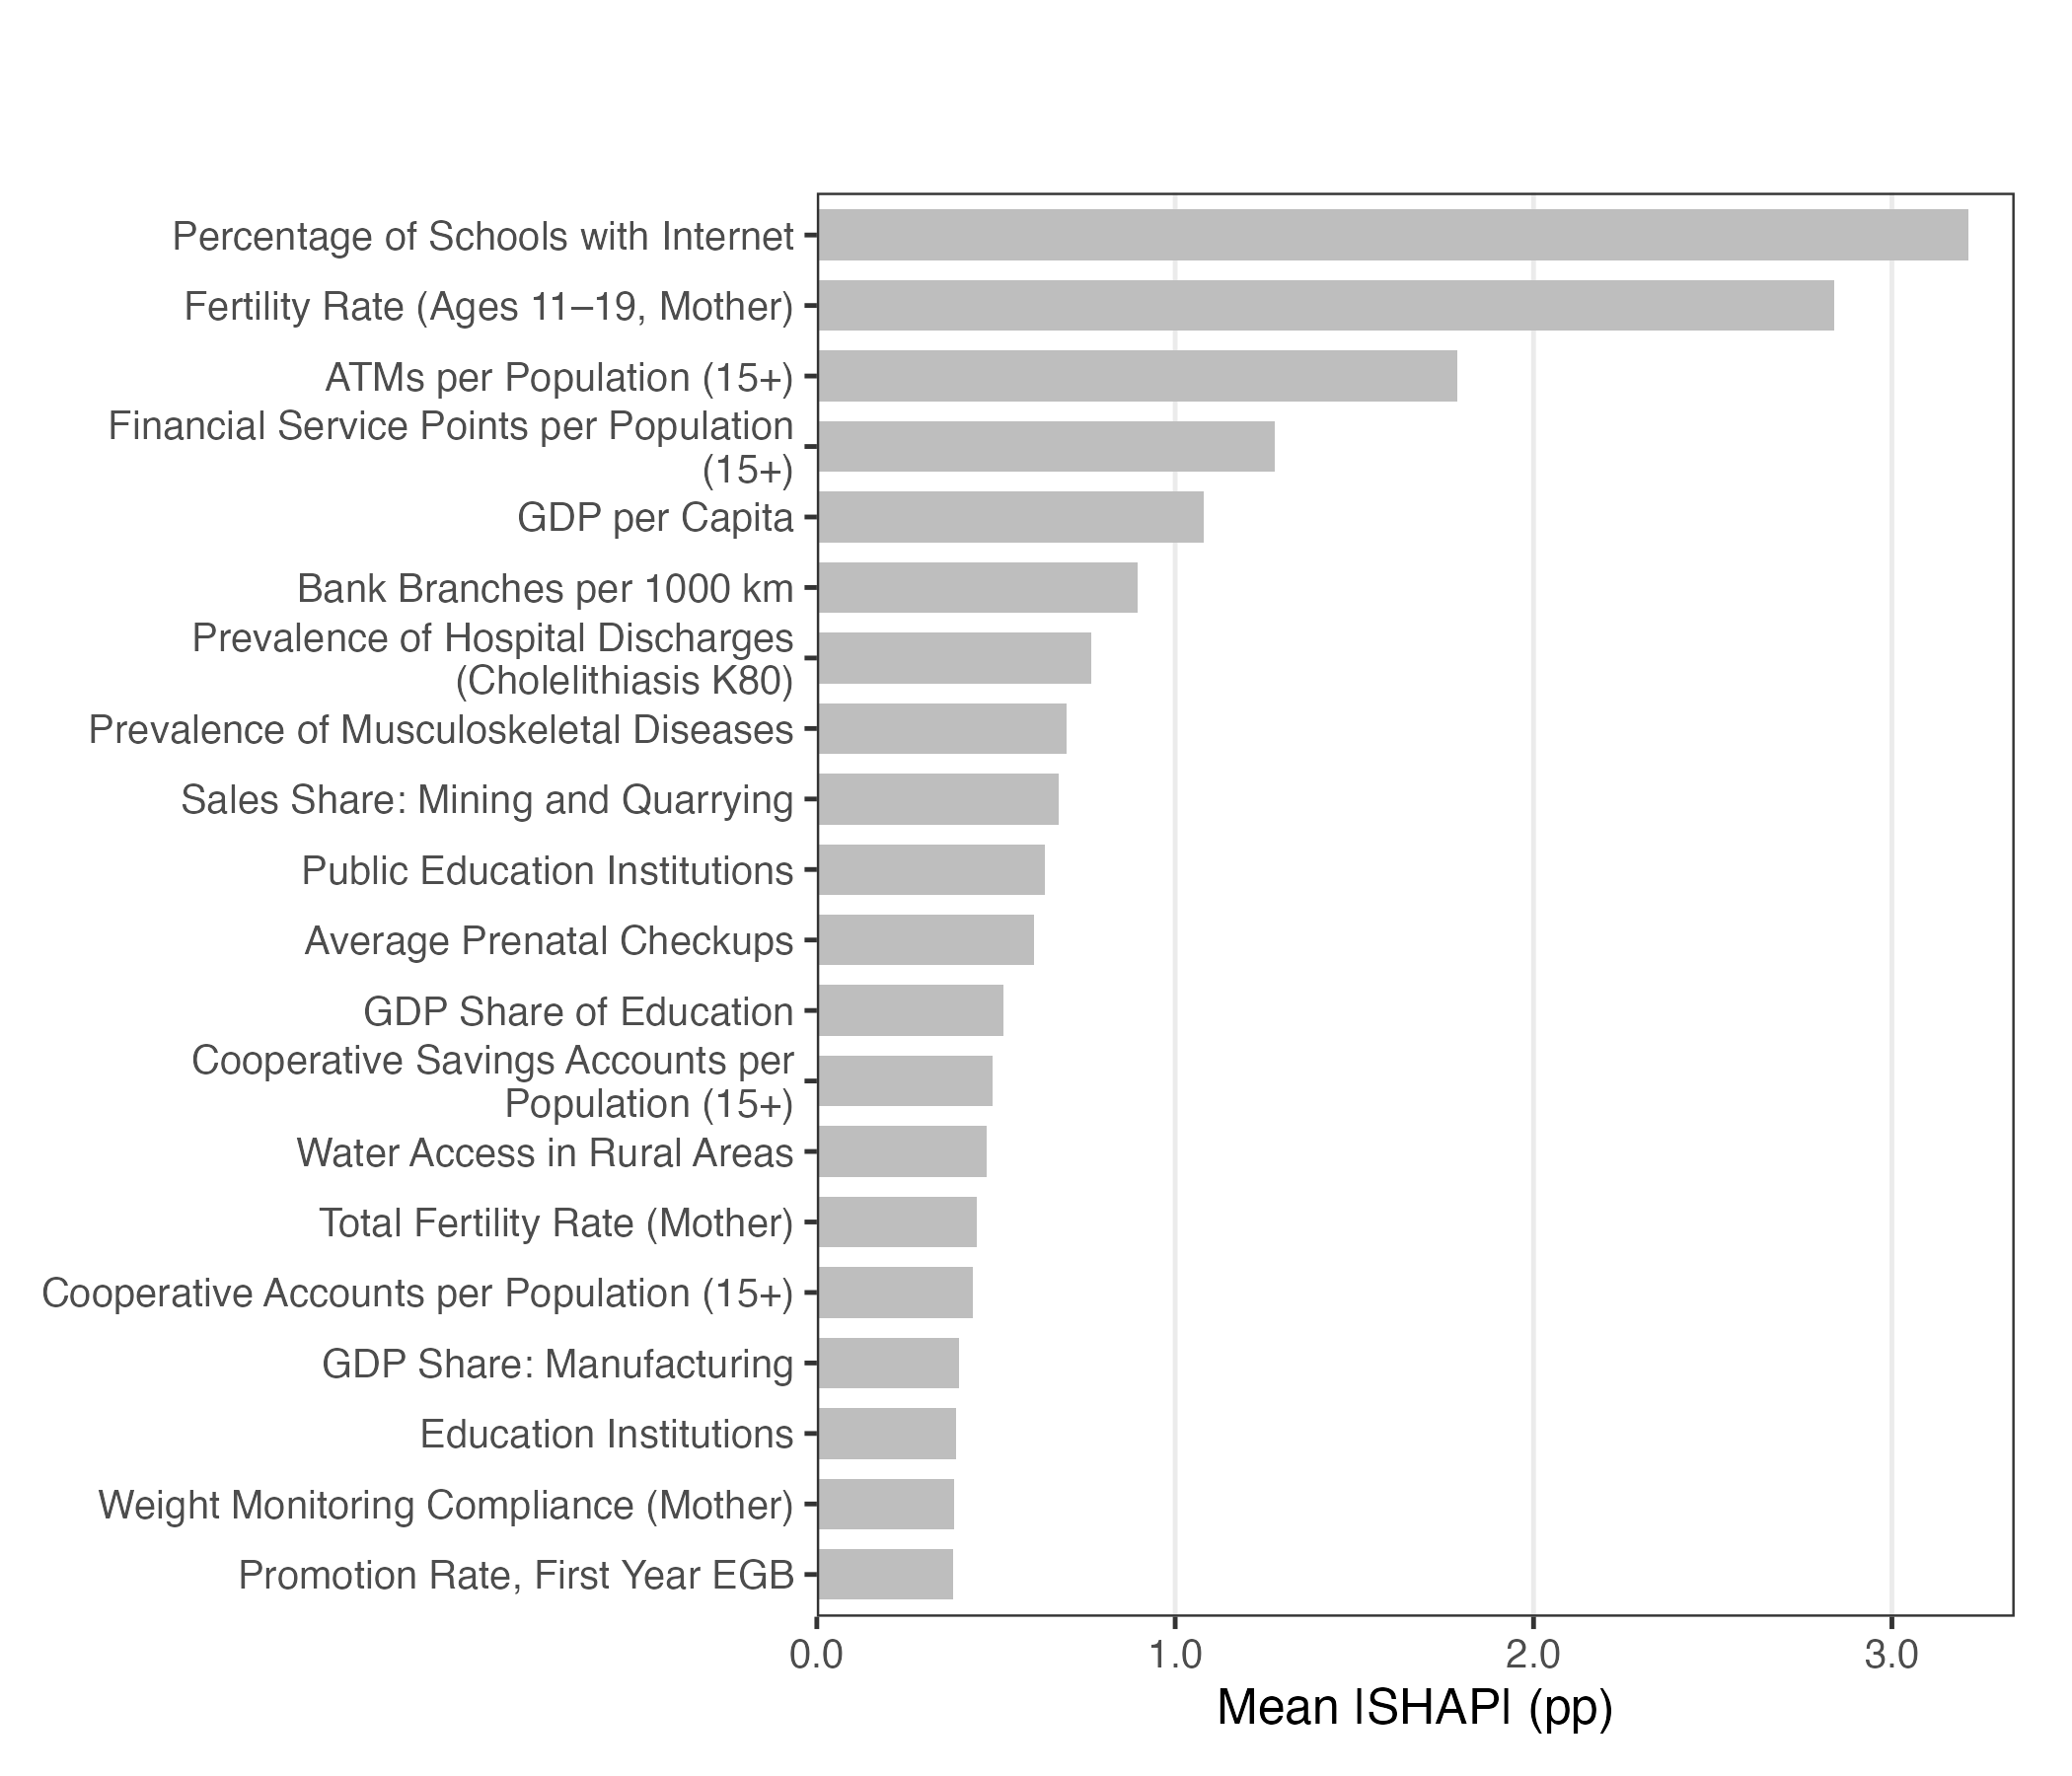
\includegraphics[width=\linewidth]{Fig10b.png}
\caption{Data scenario (2): Baseline with mobility data}
\end{subfigure}
\caption{Top 20 covariates by mean absolute SHAP value (percentage points) for each scenario (continued)}
\end{figure}

\begin{figure}[!htbp]
\ContinuedFloat
\centering
\begin{subfigure}{0.90\textwidth}
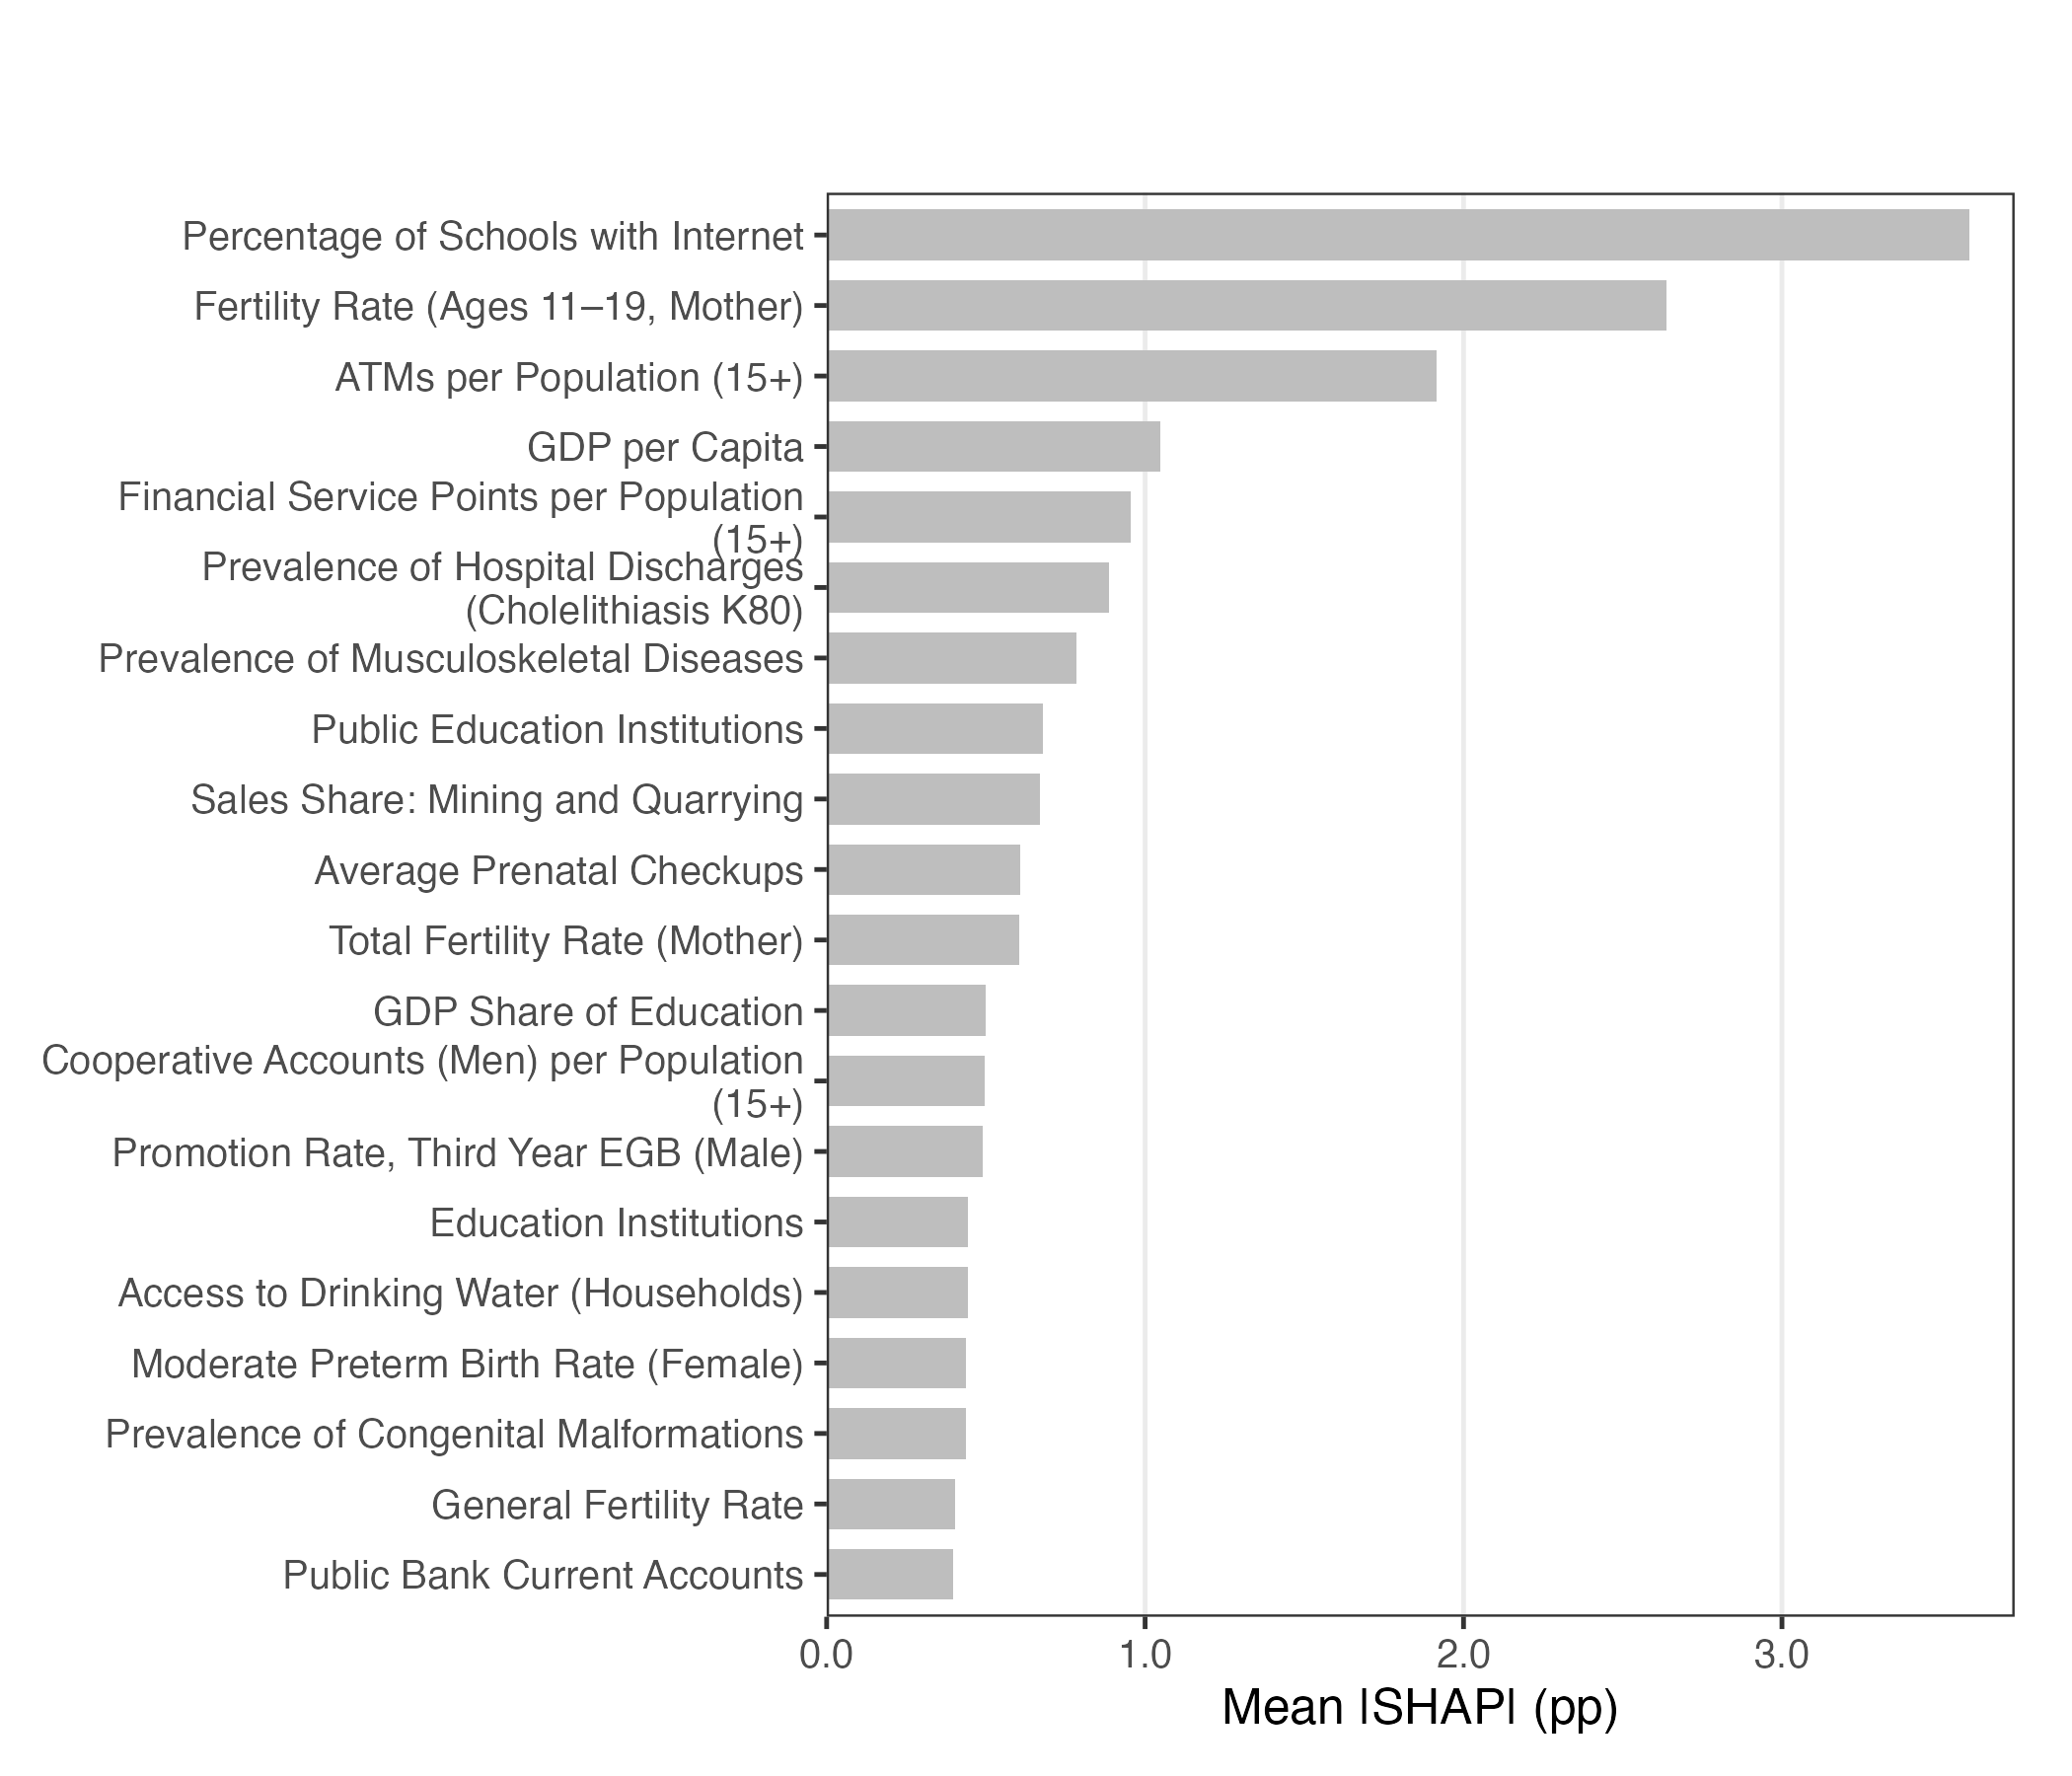
\includegraphics[width=\linewidth]{Fig10c.png}
\caption{Data scenario (3): Baseline with mobility factor}
\end{subfigure}
\caption{Top 20 covariates by mean absolute SHAP value (percentage points) for each scenario (continued)}
\end{figure}

\begin{figure}[!htbp]
\ContinuedFloat
\centering
\begin{subfigure}{0.90\textwidth}
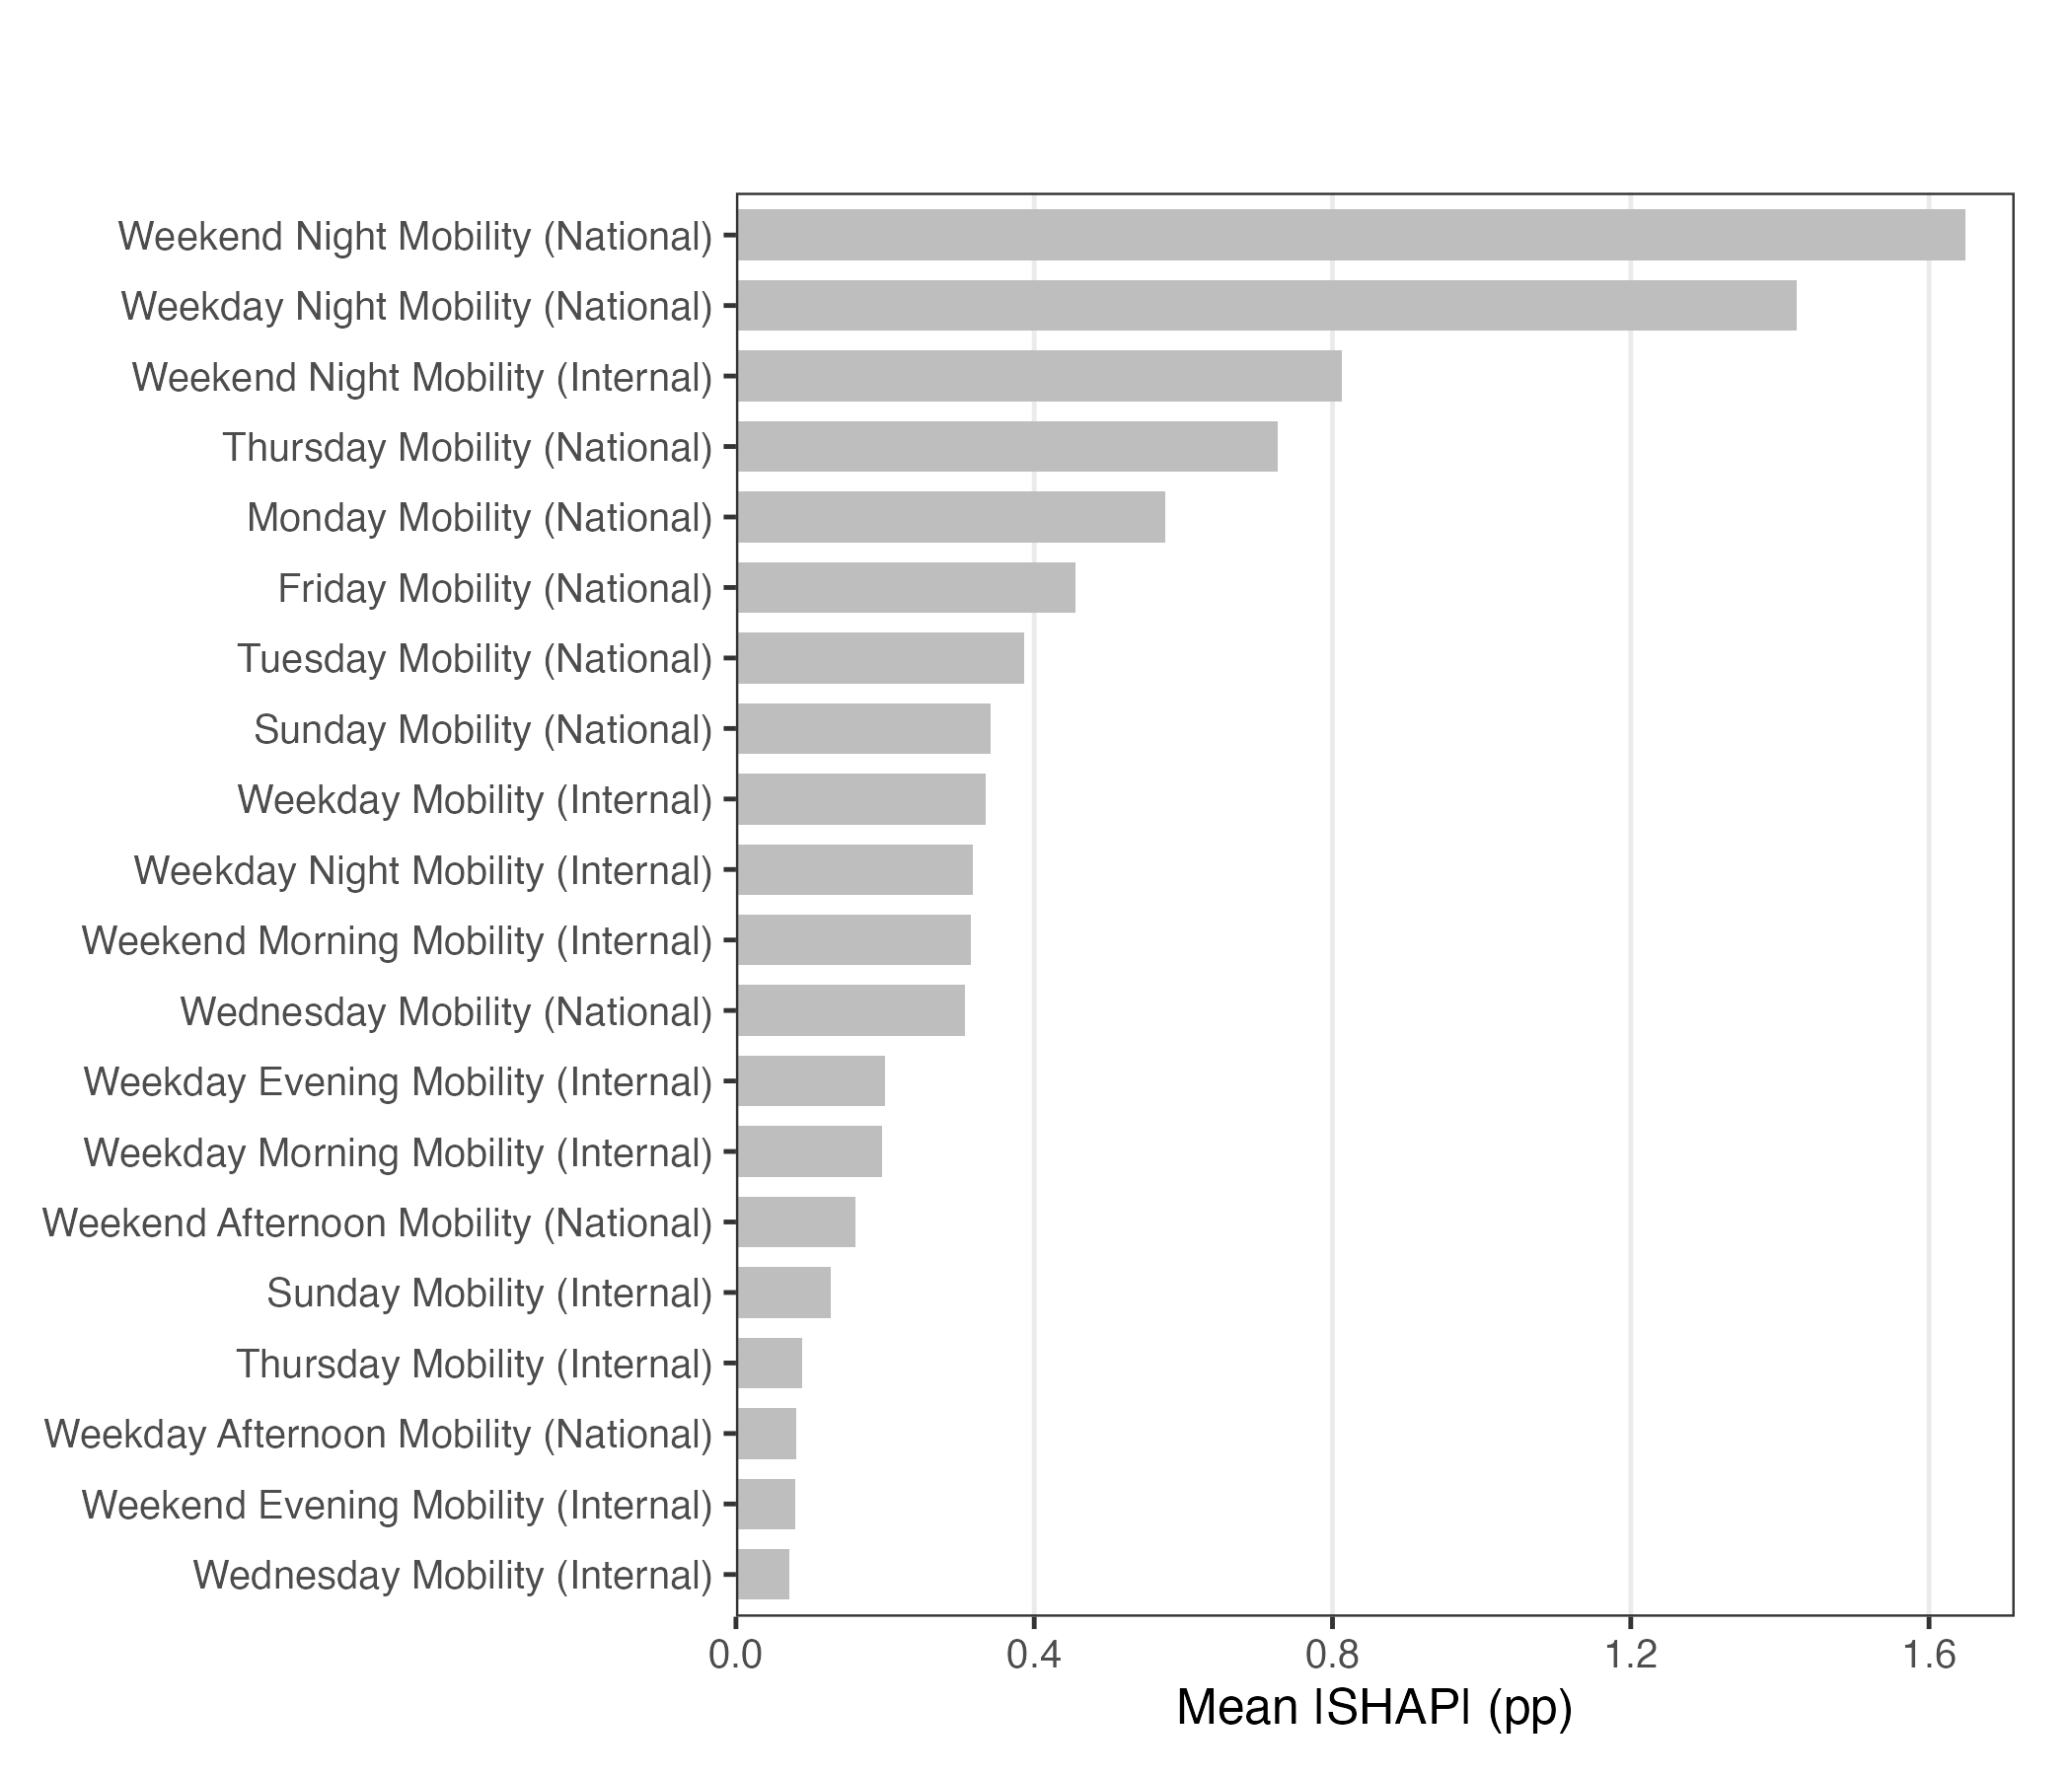
\includegraphics[width=\linewidth]{Fig10d.png}
\caption{Data scenario (4): Mobility data}
\end{subfigure}
\caption{Top 20 covariates by mean absolute SHAP value (percentage points) for each scenario (continued)}
\end{figure}

\clearpage
\section{Sensitivity to Alternative Spatial Partitions}
\label{app:repeated_spatial_cv}

To assess whether the estimated contribution of mobility data is sensitive to the choice of spatial partition, we repeated the nested five-fold spatial cross-validation procedure ten times using different spatial-clustering seeds (Table~\ref{tab:repeated-spatial-cv}). Each repetition generated one OOS prediction for each of the 218 cantons under three specifications: administrative covariates only, administrative covariates plus the mobility factor, and administrative covariates plus the 38 mobility indicators. The same outer assessment cantons were used across the three specifications within each repetition, permitting paired comparisons of prediction losses. All preprocessing operations, including standardization and construction of the mobility factor, were re-estimated within each outer training sample, and XGBoost hyperparameters were selected through inner five-fold spatial cross-validation. The exercise uses the same data-processing rules, canton exclusions, preprocessing pipeline, hyperparameter ranges, and full XGBoost specification as the main analysis; only the outer spatial partition changes.

\begin{table}[!htbp]
\centering
\small
\resizebox{\textwidth}{!}{%
\begin{tabular}{lrrrrc}
\toprule
Mobility input & Repeats & Admin. RMSE & Augmented RMSE & $\Delta$RMSE & 95\% partition range \\
\midrule
Mobility factor & 10 & 9.44 & 9.50 & 0.06 & [-0.16, 0.26] \\
38 mobility indicators & 10 & 9.44 & 9.46 & 0.02 & [-0.22, 0.24] \\
\bottomrule
\end{tabular}%
}
\caption{Paired repeated spatial cross-validation for the full XGBoost specification. $\Delta$RMSE is augmented minus administrative-only RMSE, so negative values favor mobility. The empirical range is the 2.5th--97.5th percentile range across spatial partitions and measures sensitivity to partition choice; it is not a population-sampling confidence interval}
\label{tab:repeated-spatial-cv}
\end{table}

\end{appendices}

\end{document}
